\documentclass{article}
\usepackage{graphicx} % Required for inserting images

\title{Comparison of analysis of keystone OTUs of rhizosphere of \textit{Solanum lycopersicum}: All samples, samples chosen by metadata, and samples chosen randomly.}
\author{Mario Jardon Santos}
\date{}

\begin{document}

\maketitle

\section{Introduction}
\label{intro}

For assesing the non-randomness of the results presented in ``" here they are contrasted with new analysis. 
Since there more of them the samples of rhizosphere of \textit{Solanum lycopersicum} were chosen for this task.
Firstly they were diveded according to metadata. 
These samples were classified as ``Desarrollo", ``Llenado de fruto", ``Por transplantar" and ``Llenado de fruto".
More than a half of them were classified as ``Desarrollo".
Hence they were divided by ``Desarrollo" and all the others.
There were also 10 random subsets of half (11) of the samples.

In each one of the cases a new correlation network was created and the analysis of script was done in the respective network. 
In this report are present the results of all 12 analysis and contrasted with the original one.

\section{All samples, ``Desarrollo" and Other}
\label{des_vs_no_des}

The analysis of samples labeled as ``Desarrollo" gave more candidate to keystone OTUs  than the original analysis.
Meanwhile the analysis of the complement of samples gave less of them.
In both restricted analyses there is a clear prevalence of phyla \textit{Actinomycetota} and \textit{Pseudomonadota}. 
More abundant genera in the analysis of ``Desarrollo" samples are \textit{Pseudomonas, Deinococcus} and \textit{Corynebacterium}. 
In the less diverse analysis of the other samples the most abundant genus is \textit{Pseudomonas}. 

As can be seen in Figures \ref{mean_median_tomate_desarrollo.csv} and  \ref{mean_median_tomate_no_desarrollo.csv} both partial analyses gave OTUs whose relative abundance tends to be between the median and the mean relative abundance of all other OTUs across samples.
This ressembles the distribution of keystone OTUs of the samples of \textit{Capsicum} and \textit{Zea mays} and contrasts that of the first analysis of the samples of \textit{Solanum lycopersicum}.

% latex table generated in R 3.6.3 by xtable 1.8-4 package
% Wed Jan 17 12:52:14 2024
\begin{table}[ht]
\centering
\begin{tabular}{rlrrr}
  \hline
 & OTU & MeanRA & MedianRA & SE \\ 
  \hline
1479019 & Methylobacterium sp. C & 0.00007633 & 0.00007547 & 0.00000216 \\ 
  299262 & Tateyamaria omphali & 0.00010673 & 0.00010456 & 0.00000349 \\ 
  1858609 & Acidovorax sp. T & 0.00011493 & 0.00010232 & 0.00000968 \\ 
  1658672 & Ottowia sp. oral taxon 89 & 0.00013825 & 0.00013775 & 0.00000374 \\ 
  2202141 & Chromobacterium phragmiti & 0.00011981 & 0.00011471 & 0.00000336 \\ 
  658630 & Pseudomonas sp. CMR5 & 0.00008522 & 0.00007885 & 0.00000672 \\ 
  1881017 & Pseudomonas sp. 7SR & 0.00008174 & 0.00006956 & 0.00000750 \\ 
  2054919 & Pseudomonas sp. S09G 35 & 0.00004755 & 0.00004597 & 0.00000304 \\ 
  2774873 & Pseudomonas sp. ADP & 0.00005952 & 0.00004786 & 0.00000683 \\ 
  2219057 & Pseudomonas sp. LG1E & 0.00003061 & 0.00002850 & 0.00000180 \\ 
  1898684 & Pseudomonas sp. LPH & 0.00004548 & 0.00002501 & 0.00001203 \\ 
  2590776 & Pseudomonas sp. NIBRBAC00050277 & 0.00002328 & 0.00002083 & 0.00000190 \\ 
  2774459 & Pseudomonas sp. IzPS5 & 0.00002884 & 0.00002700 & 0.00000225 \\ 
  200450 & Pseudomonas triviali & 0.00007870 & 0.00007535 & 0.00000487 \\ 
  183795 & Pseudomonas mediterrane & 0.00006965 & 0.00005698 & 0.00000853 \\ 
  29442 & Pseudomonas tolaasi & 0.00004854 & 0.00004475 & 0.00000300 \\ 
  75588 & Pseudomonas libanensi & 0.00002296 & 0.00001980 & 0.00000186 \\ 
  1691904 & Pseudomonas sedimini & 0.00007117 & 0.00004577 & 0.00001392 \\ 
  1853130 & Pseudomonas silesiensi & 0.00005116 & 0.00004823 & 0.00000342 \\ 
  1434072 & Halopseudomonas salegen & 0.00005960 & 0.00005114 & 0.00000621 \\ 
  1073999 & Cronobacter condimenti & 0.00002925 & 0.00002816 & 0.00000115 \\ 
  2666185 & Spiribacter sp. 243 & 0.00011615 & 0.00011621 & 0.00000390 \\ 
  2661612 & Pseudodesulfovibrio & 0.00004334 & 0.00004365 & 0.00000183 \\ 
  1894 & Kitasatospora aureofacien & 0.00007564 & 0.00007907 & 0.00000520 \\ 
  300019 & Microbacterium paludicol & 0.00003330 & 0.00002934 & 0.00000293 \\ 
  256701 & Glutamicibacter arilaitensi & 0.00004168 & 0.00004316 & 0.00000315 \\ 
  1630135 & Dermabacter vaginali & 0.00007216 & 0.00007167 & 0.00000313 \\ 
  83262 & Mycobacteroides immunogenu & 0.00011016 & 0.00010334 & 0.00000493 \\ 
  441500 & Corynebacterium timonens & 0.00009727 & 0.00009133 & 0.00000364 \\ 
  43771 & Corynebacterium urealyticu & 0.00006312 & 0.00006273 & 0.00000245 \\ 
  43770 & Corynebacterium striatu & 0.00004302 & 0.00004224 & 0.00000233 \\ 
  203263 & Corynebacterium aquila & 0.00003411 & 0.00003577 & 0.00000180 \\ 
  2609299 & Actinobaculum & 0.00004557 & 0.00004722 & 0.00000257 \\ 
  35760 & Bifidobacterium choerinu & 0.00011989 & 0.00012381 & 0.00000479 \\ 
  1335613 & Gordonibacter urolithinfacien & 0.00009591 & 0.00009744 & 0.00000181 \\ 
  604330 & Parafannyhessea umbonat & 0.00011704 & 0.00011906 & 0.00000404 \\ 
  1871022 & Parolsenella massiliensi & 0.00007758 & 0.00007810 & 0.00000239 \\ 
  365617 & Paenibacillus sabina & 0.00004839 & 0.00004879 & 0.00000176 \\ 
  2610894 & Flintibacter & 0.00004748 & 0.00004828 & 0.00000247 \\ 
  2614128 & Clostridium & 0.00005019 & 0.00004795 & 0.00000247 \\ 
  42837 &  Ammonife & 0.00007226 & 0.00007016 & 0.00000298 \\ 
  92942 & Nostoc lincki & 0.00002378 & 0.00001464 & 0.00000550 \\ 
  2618749 & Scytonema & 0.00008482 & 0.00008961 & 0.00000847 \\ 
  980427 & Deinococcus wulumuqiensi & 0.00014906 & 0.00014494 & 0.00000394 \\ 
  1299 & Deinococcus radioduran & 0.00012662 & 0.00012342 & 0.00000325 \\ 
  310783 & Deinococcus desert & 0.00009394 & 0.00009060 & 0.00000429 \\ 
  454171 & Chthonomonas calidirose & 0.00007864 & 0.00007652 & 0.00000248 \\ 
  290174 & Aquimarin  & 0.00001626 & 0.00001591 & 0.00000115 \\ 
  869211 & Spirochaeta thermophila & 0.00002979 & 0.00002963 & 0.00000142 \\ 
  62320 & Haloterrigena turkmenic & 0.00008121 & 0.00008087 & 0.00000363 \\ 
  370324 & Natrinema longu & 0.00005274 & 0.00005464 & 0.00000214 \\ 
  13769 & Natrialba magadi & 0.00007369 & 0.00007005 & 0.00000315 \\ 
  1175445 & Methanocella arvoryza & 0.00003724 & 0.00003540 & 0.00000206 \\ 
  1826872 & Candidatus Nitrosocosmicus hydrocol & 0.00007780 & 0.00005223 & 0.00001720 \\ 
   \hline
\end{tabular}
\caption{Keystone OTUs of } 
\end{table}

\begin{table}[ht]
\centering
\begin{tabular}{rlrrr}
  \hline
 & OTU & MeanRA & MedianRA & SE \\ 
  \hline
419610 & Methylorubrum extorquens & 0.00006533 & 0.00005353 & 0.00001571 \\ 
  32009 & Burkholderia gladioli & 0.00004414 & 0.00004435 & 0.00000339 \\ 
  640081 & Azospira oryzae & 0.00006336 & 0.00005796 & 0.00000936 \\ 
  2706126 & Pseudomonas sp. OIL- & 0.00005744 & 0.00005843 & 0.00000328 \\ 
  2726989 & Pseudomonas sp. gcc2 & 0.00005071 & 0.00004922 & 0.00000329 \\ 
  76760 & Pseudomonas rhodesia & 0.00004632 & 0.00004114 & 0.00000576 \\ 
  553151 & Halopseudomonas pelagi & 0.00005750 & 0.00006352 & 0.00000567 \\ 
  219572 & Pseudomonas antarctic & 0.00004038 & 0.00003570 & 0.00000376 \\ 
  163011 & Pseudomonas lin & 0.00004752 & 0.00003619 & 0.00001561 \\ 
  64187 & Xanthomonas oryzae & 0.00004090 & 0.00003884 & 0.00000303 \\ 
  349967 & Yersinia mollaretii & 0.00000693 & 0.00000691 & 0.00000067 \\ 
  213554 & Halomonas campaniensi & 0.00000240 & 0.00000200 & 0.00000086 \\ 
  28084 & Legionella cherri & 0.00000718 & 0.00000570 & 0.00000212 \\ 
  92644 & Streptomyces malaysiensi & 0.00003218 & 0.00003575 & 0.00000554 \\ 
  67260 & Streptomyces cinereorube & 0.00002301 & 0.00002338 & 0.00000287 \\ 
  556325 & Neomicrococcus aestuari & 0.00003666 & 0.00003595 & 0.00000502 \\ 
  1520670 & [Mycobacterium] stephanolepidi & 0.00004888 & 0.00004736 & 0.00000707 \\ 
  33035 & Blautia product & 0.00001165 & 0.00001107 & 0.00000076 \\ 
  2214 & Methanosarcina acetivoran & 0.00000506 & 0.00000397 & 0.00000123 \\ 
  1903276 & Candidatus Nitrosotalea okcheonensi & 0.00001042 & 0.00000944 & 0.00000316 \\ 
  1410606 & Candidatus Nitrosopelagicus brevi & 0.00000579 & 0.00000431 & 0.00000191 \\ 
  2271 & Thermoproteus tena & 0.00000577 & 0.00000552 & 0.00000157 \\ 
   \hline
\end{tabular}
\caption{Keystone OTUs of } 
\end{table}

\begin{table}[ht]
\centering
\begin{tabular}{rlrrr}
  \hline
 & OTU & MeanRA & MedianRA & SE \\ 
  \hline
1458461 & Candidatus Phaeomarinobacter ectocarp & 0.00010969 & 0.00011098 & 0.00000502 \\ 
  664962 & Azospirillum sp. TSH5 & 0.00025600 & 0.00026473 & 0.00000964 \\ 
  265959 & Komagataeibacter saccharivoran & 0.00008108 & 0.00008263 & 0.00000301 \\ 
  540747 & Roseovarius indicu & 0.00028936 & 0.00028946 & 0.00000572 \\ 
  311180 & Alloyangia pacific & 0.00027703 & 0.00027666 & 0.00000503 \\ 
  101571 & Burkholderia ubonensi & 0.00030111 & 0.00029961 & 0.00000970 \\ 
  179879 & Burkholderia anthin & 0.00020302 & 0.00019456 & 0.00000805 \\ 
  1637853 & Burkholderia sp. NRF60-BP & 0.00007520 & 0.00007616 & 0.00000330 \\ 
  28450 & Burkholderia pseudomalle & 0.00028979 & 0.00027932 & 0.00001318 \\ 
  2735433 & Paraburkholderia sp. PGU1 & 0.00014528 & 0.00014581 & 0.00000776 \\ 
  1417228 & Paraburkholderia phytofirmans & 0.00012977 & 0.00012522 & 0.00000523 \\ 
  134537 & Paraburkholderia fungoru & 0.00023287 & 0.00022773 & 0.00001276 \\ 
  1761016 & Paraburkholderia caffeinilytic & 0.00016107 & 0.00016257 & 0.00000629 \\ 
  656178 & Pandoraea vervact & 0.00017448 & 0.00017640 & 0.00000579 \\ 
  2320867 & Pseudomonas caverna & 0.00024406 & 0.00019991 & 0.00003192 \\ 
  1931241 & Halopseudomonas phragmiti & 0.00007181 & 0.00007016 & 0.00000402 \\ 
  364197 & Pseudomonas pohangensi & 0.00007540 & 0.00006487 & 0.00000571 \\ 
  46677 & Pseudomonas agaric & 0.00005228 & 0.00004649 & 0.00000390 \\ 
  549 & Pantoea agglomeran & 0.00004466 & 0.00004297 & 0.00000220 \\ 
  2819280 & Acidihalobacter yilgarnensi & 0.00011547 & 0.00011858 & 0.00000483 \\ 
  550540 & Ferrimonas balearica & 0.00006810 & 0.00006783 & 0.00000238 \\ 
  145458 & Rathayibacter toxicu & 0.00004330 & 0.00004355 & 0.00000240 \\ 
  2649579 & Kocuria & 0.00018552 & 0.00018052 & 0.00000885 \\ 
  85085 & Pseudarthrobacter chlorophenolicu & 0.00020598 & 0.00014120 & 0.00003691 \\ 
  121292 & Pseudarthrobacter sulfonivoran & 0.00009350 & 0.00007732 & 0.00001262 \\ 
  2593973 & Ornithinimicrobium pratens & 0.00022492 & 0.00022325 & 0.00000936 \\ 
  126673 & Mycolicibacterium doricu & 0.00017894 & 0.00018047 & 0.00000638 \\ 
  1661 & Trueperella pyogene & 0.00005859 & 0.00006066 & 0.00000199 \\ 
  49283 & Paenibacillus thiaminolyticu & 0.00009204 & 0.00009356 & 0.00000363 \\ 
  186192 & Marinithermus hydrothermali & 0.00021079 & 0.00020931 & 0.00000722 \\ 
  2509675 & Ktedonosporobacter rubrisol & 0.00012649 & 0.00011891 & 0.00001055 \\ 
  1005039 & Fimbriimonas ginsengisol & 0.00029796 & 0.00029765 & 0.00001108 \\ 
  125 & Pirellula staley & 0.00027144 & 0.00023236 & 0.00001909 \\ 
  128 & Isosphaera pallid & 0.00026970 & 0.00026452 & 0.00001368 \\ 
  2703788 & Edaphobacter sp. 12200R-10 & 0.00028184 & 0.00021699 & 0.00007508 \\ 
  2643768 & Halorussus  & 0.00011966 & 0.00012219 & 0.00000403 \\ 
  1353260 & Candidatus Nitrosocosmicus oleophilu & 0.00009234 & 0.00008950 & 0.00000769 \\ 
   \hline
\end{tabular}
\caption{Keystone OTUs of \textit{Solanum lycopersicum} with mean and median relative abundance and standard error.}
\label{tabla_tomate}
\end{table}



\begin{figure}
\centering
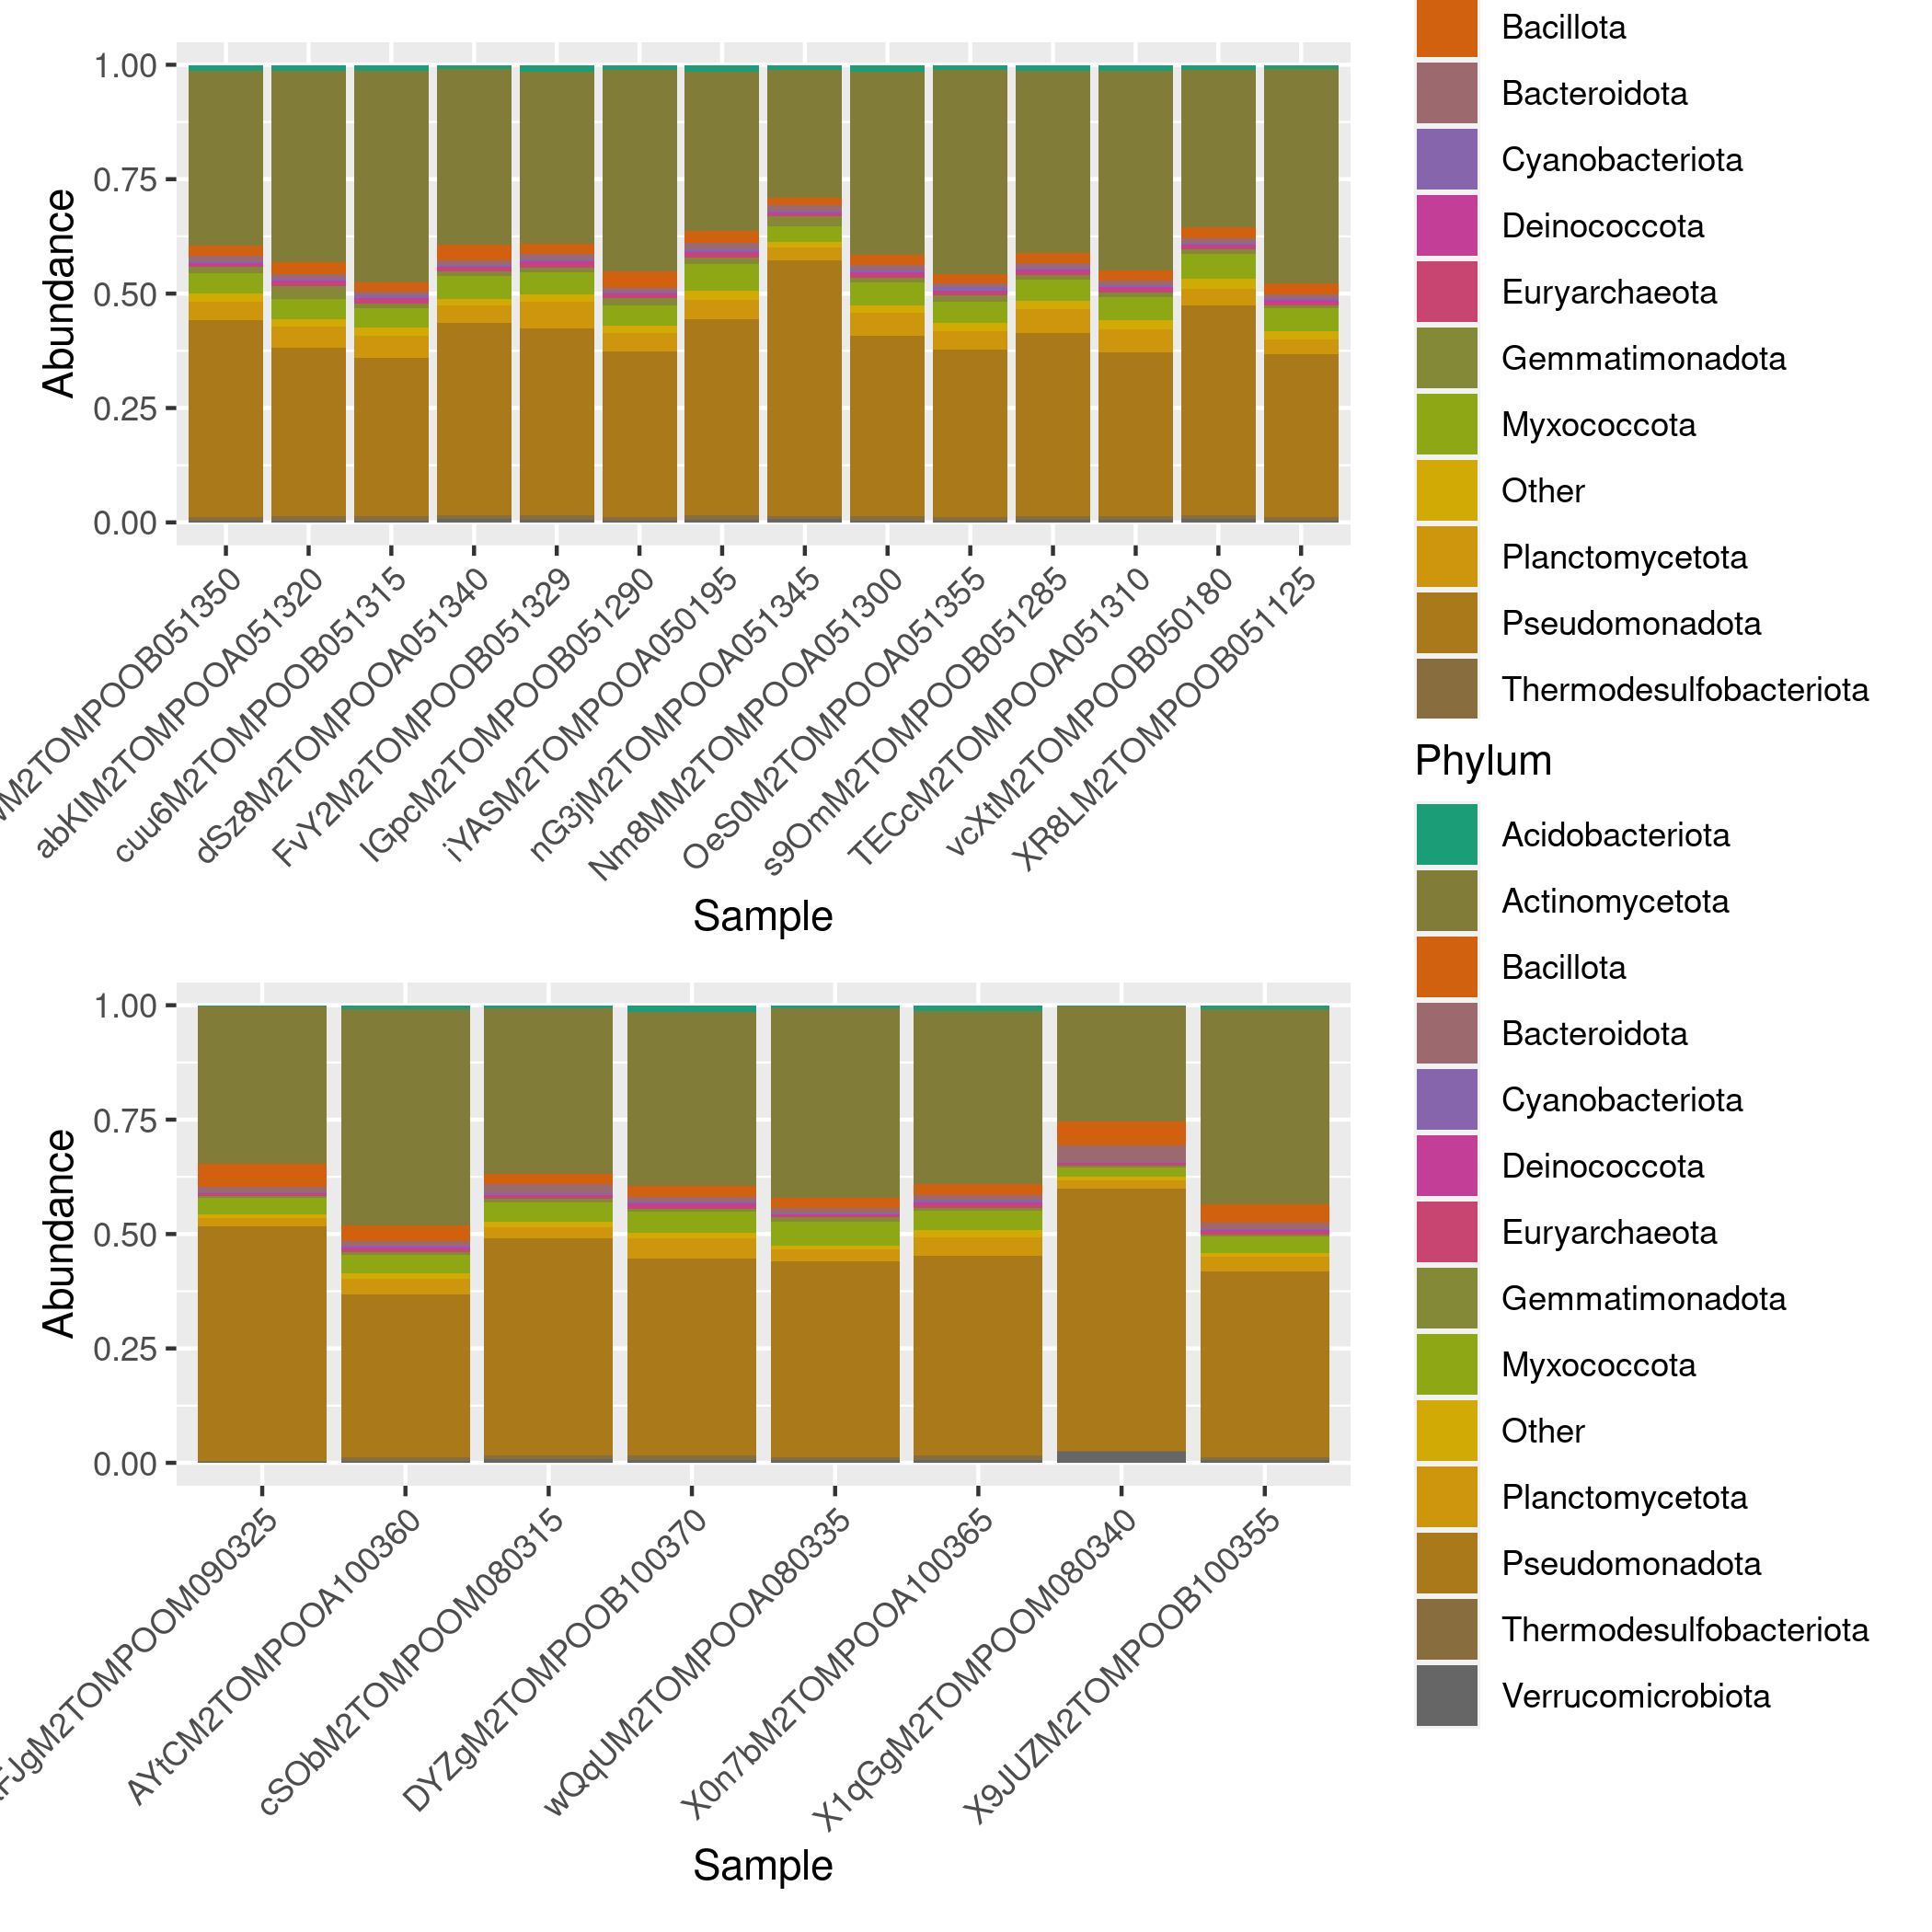
\includegraphics[scale=0.8]{tomate_desarrollo.csv_tomate_no_desarrollo.csv_relative_abundance_Phylum.png}
\caption{Comparison of reports of ``Desarrollo" and ``No desarrolo" by Phylum}
\end{figure}


\begin{figure}
\centering
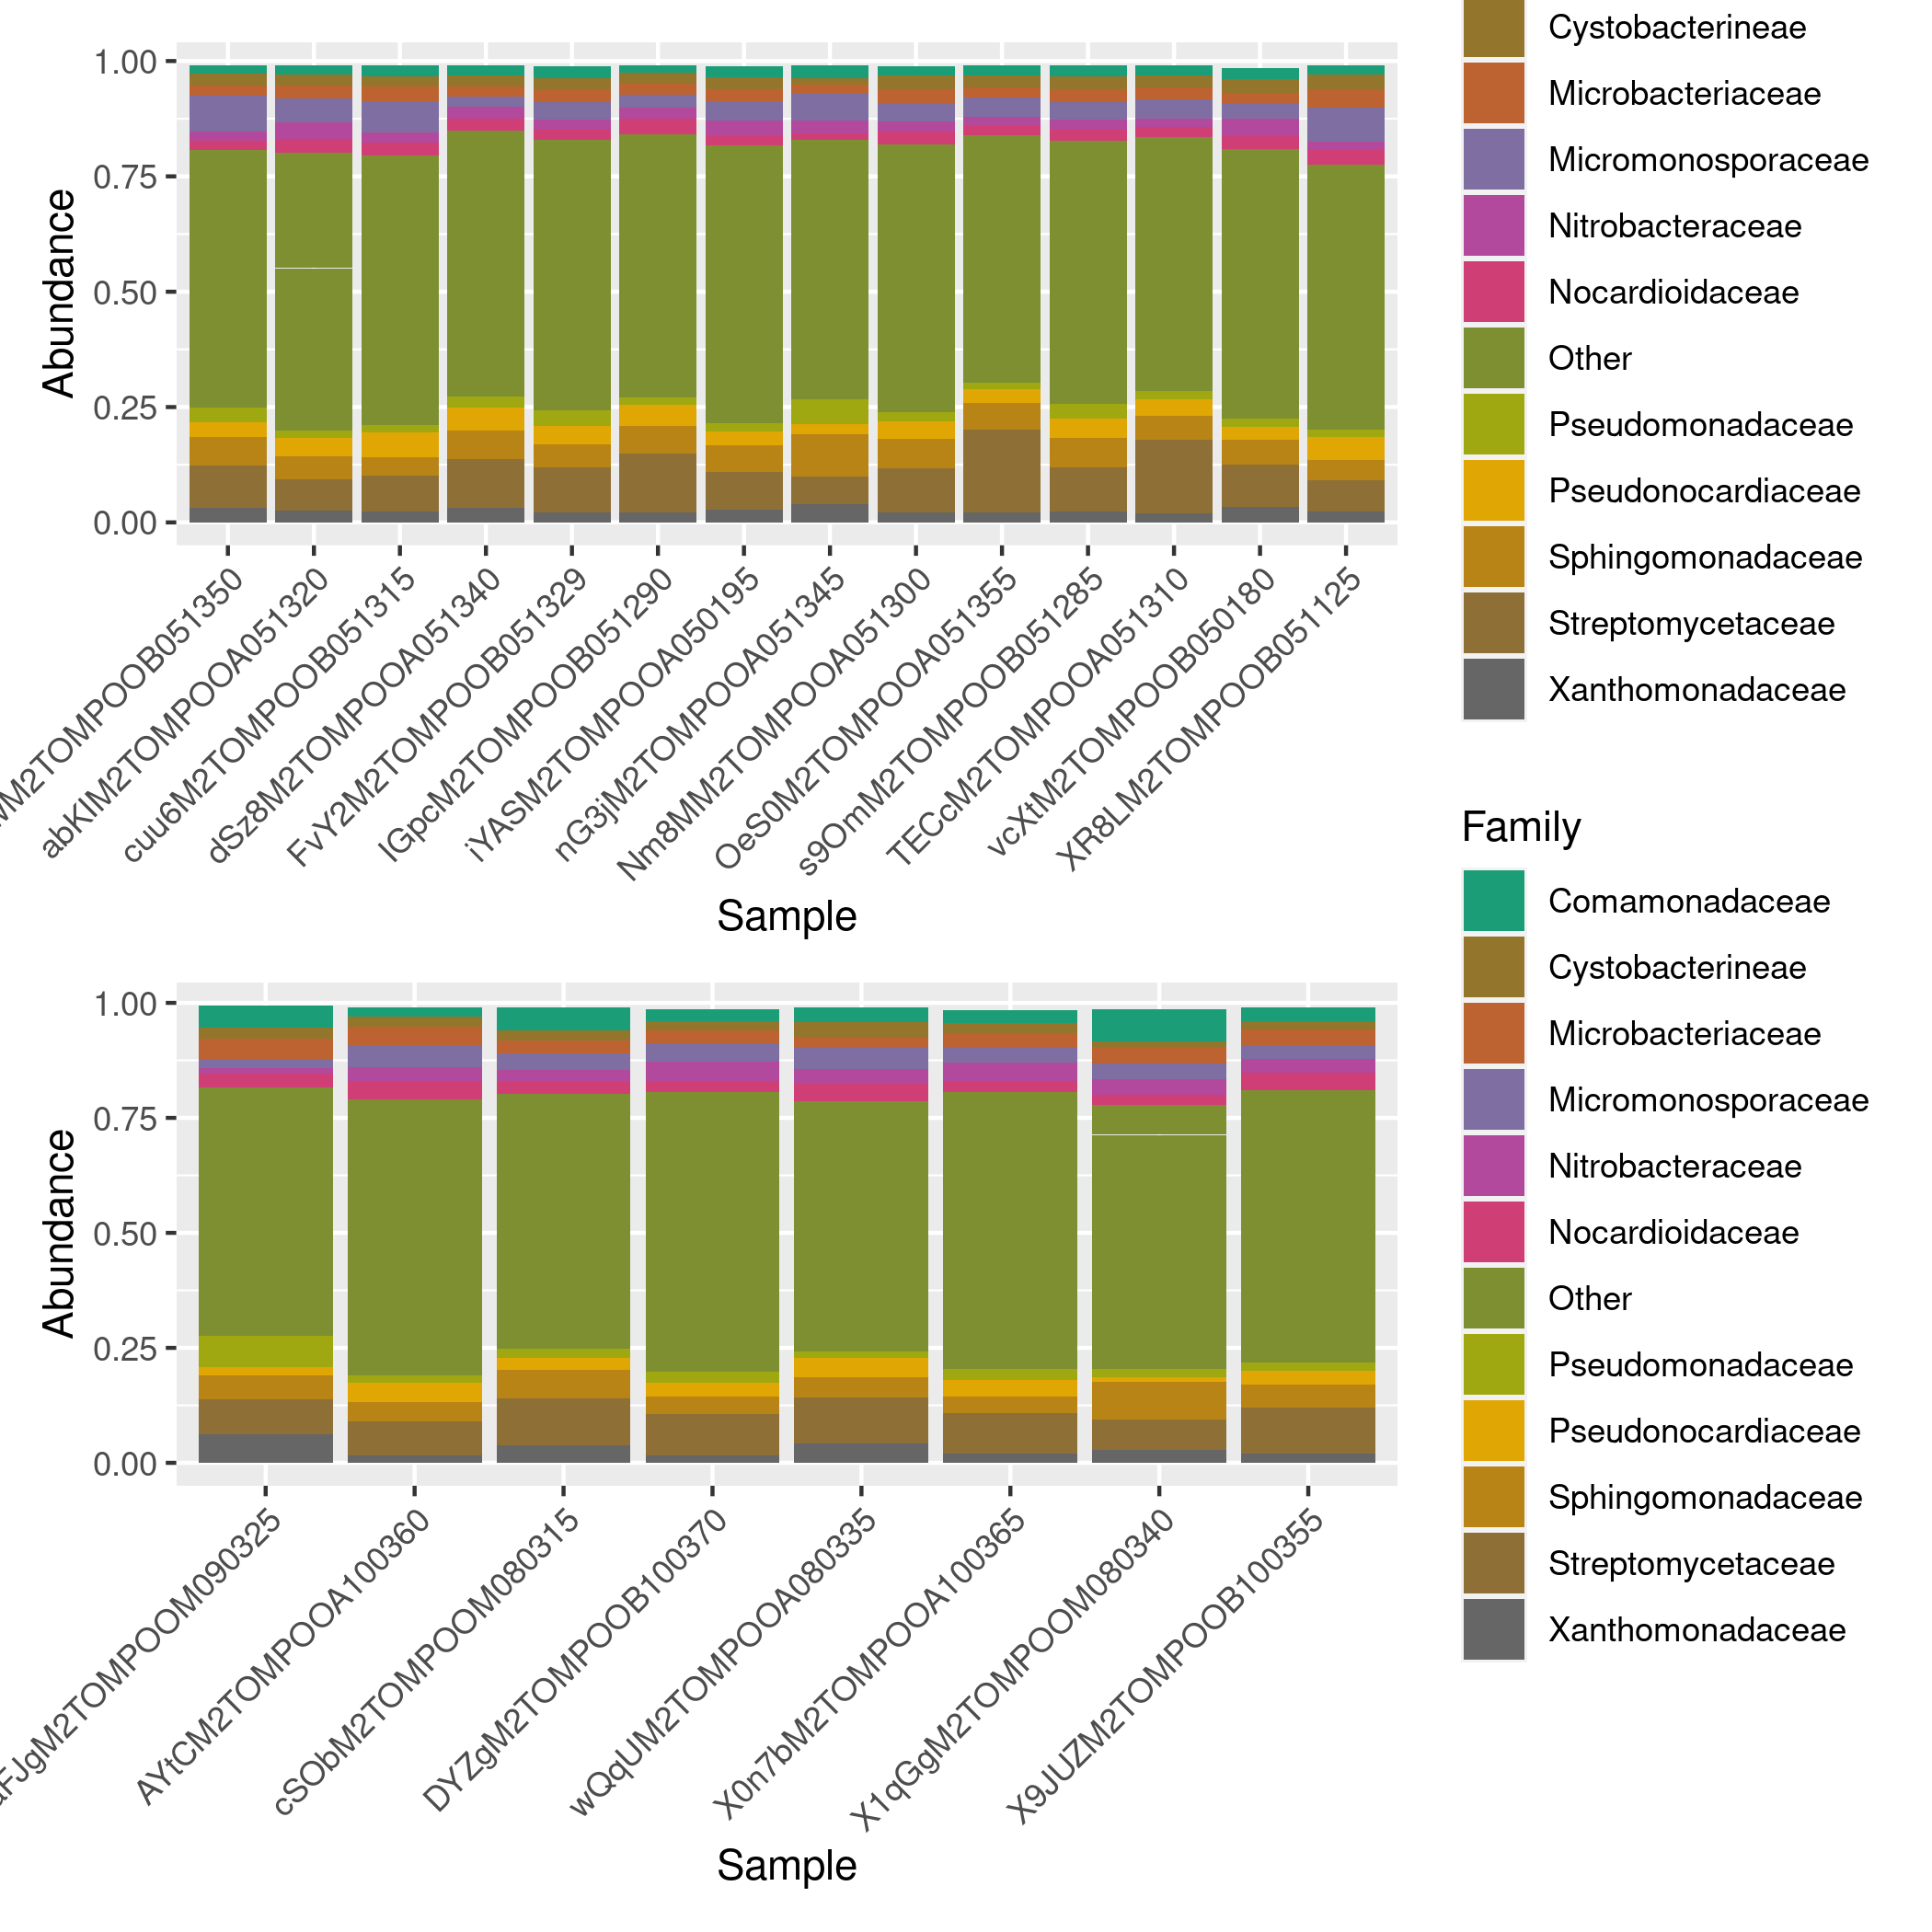
\includegraphics[scale=0.8]{tomate_desarrollo.csv_tomate_no_desarrollo.csv_relative_abundance_Family.png}
\caption{Comparison of reports of ``Desarrollo" and ``No desarrolo" by Family}
\end{figure}

\begin{figure}
    \centering
    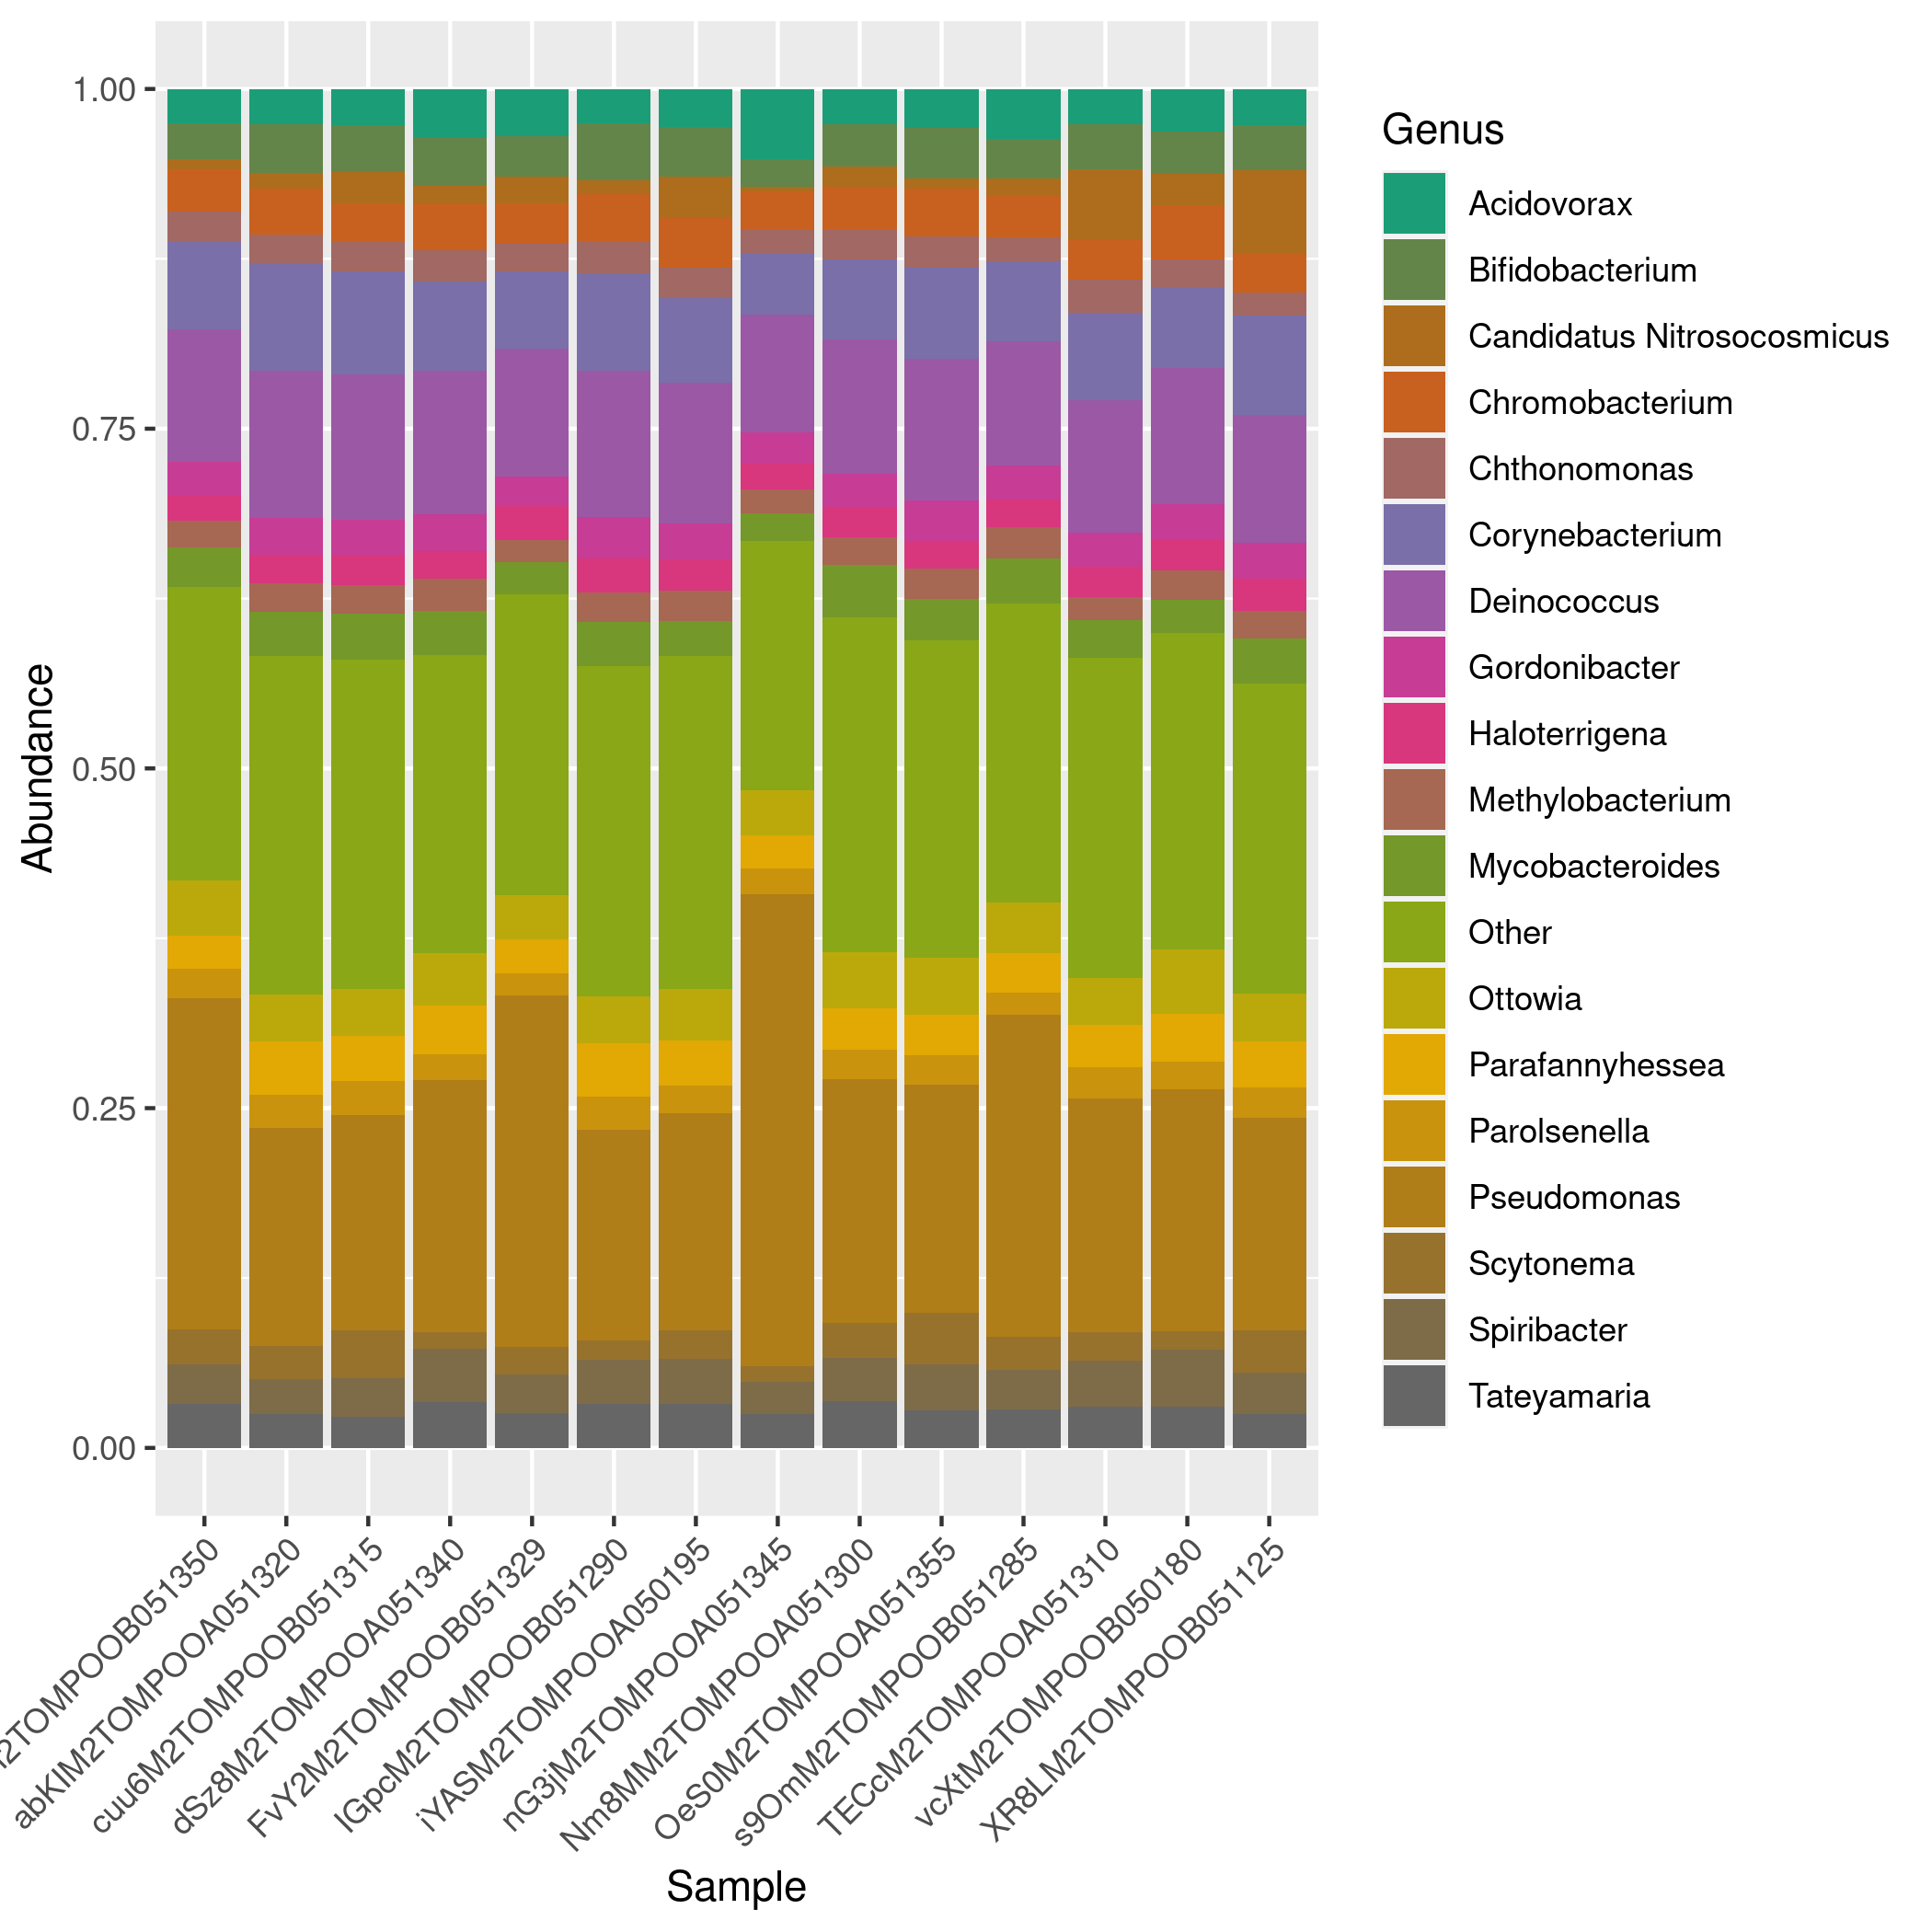
\includegraphics[scale = 0.8]{tomate_desarrollo.csv_relative_abundance_Genus.png}
    \caption{Relative abundance by genera of keystone OTUs in rhizosphere samples of \textit{Solanum lycopersicum} labeled as ``Desarrollo".}
    \label{tomate_desarrollo_key_abundance_family}
\end{figure}


\begin{figure}
    \centering
    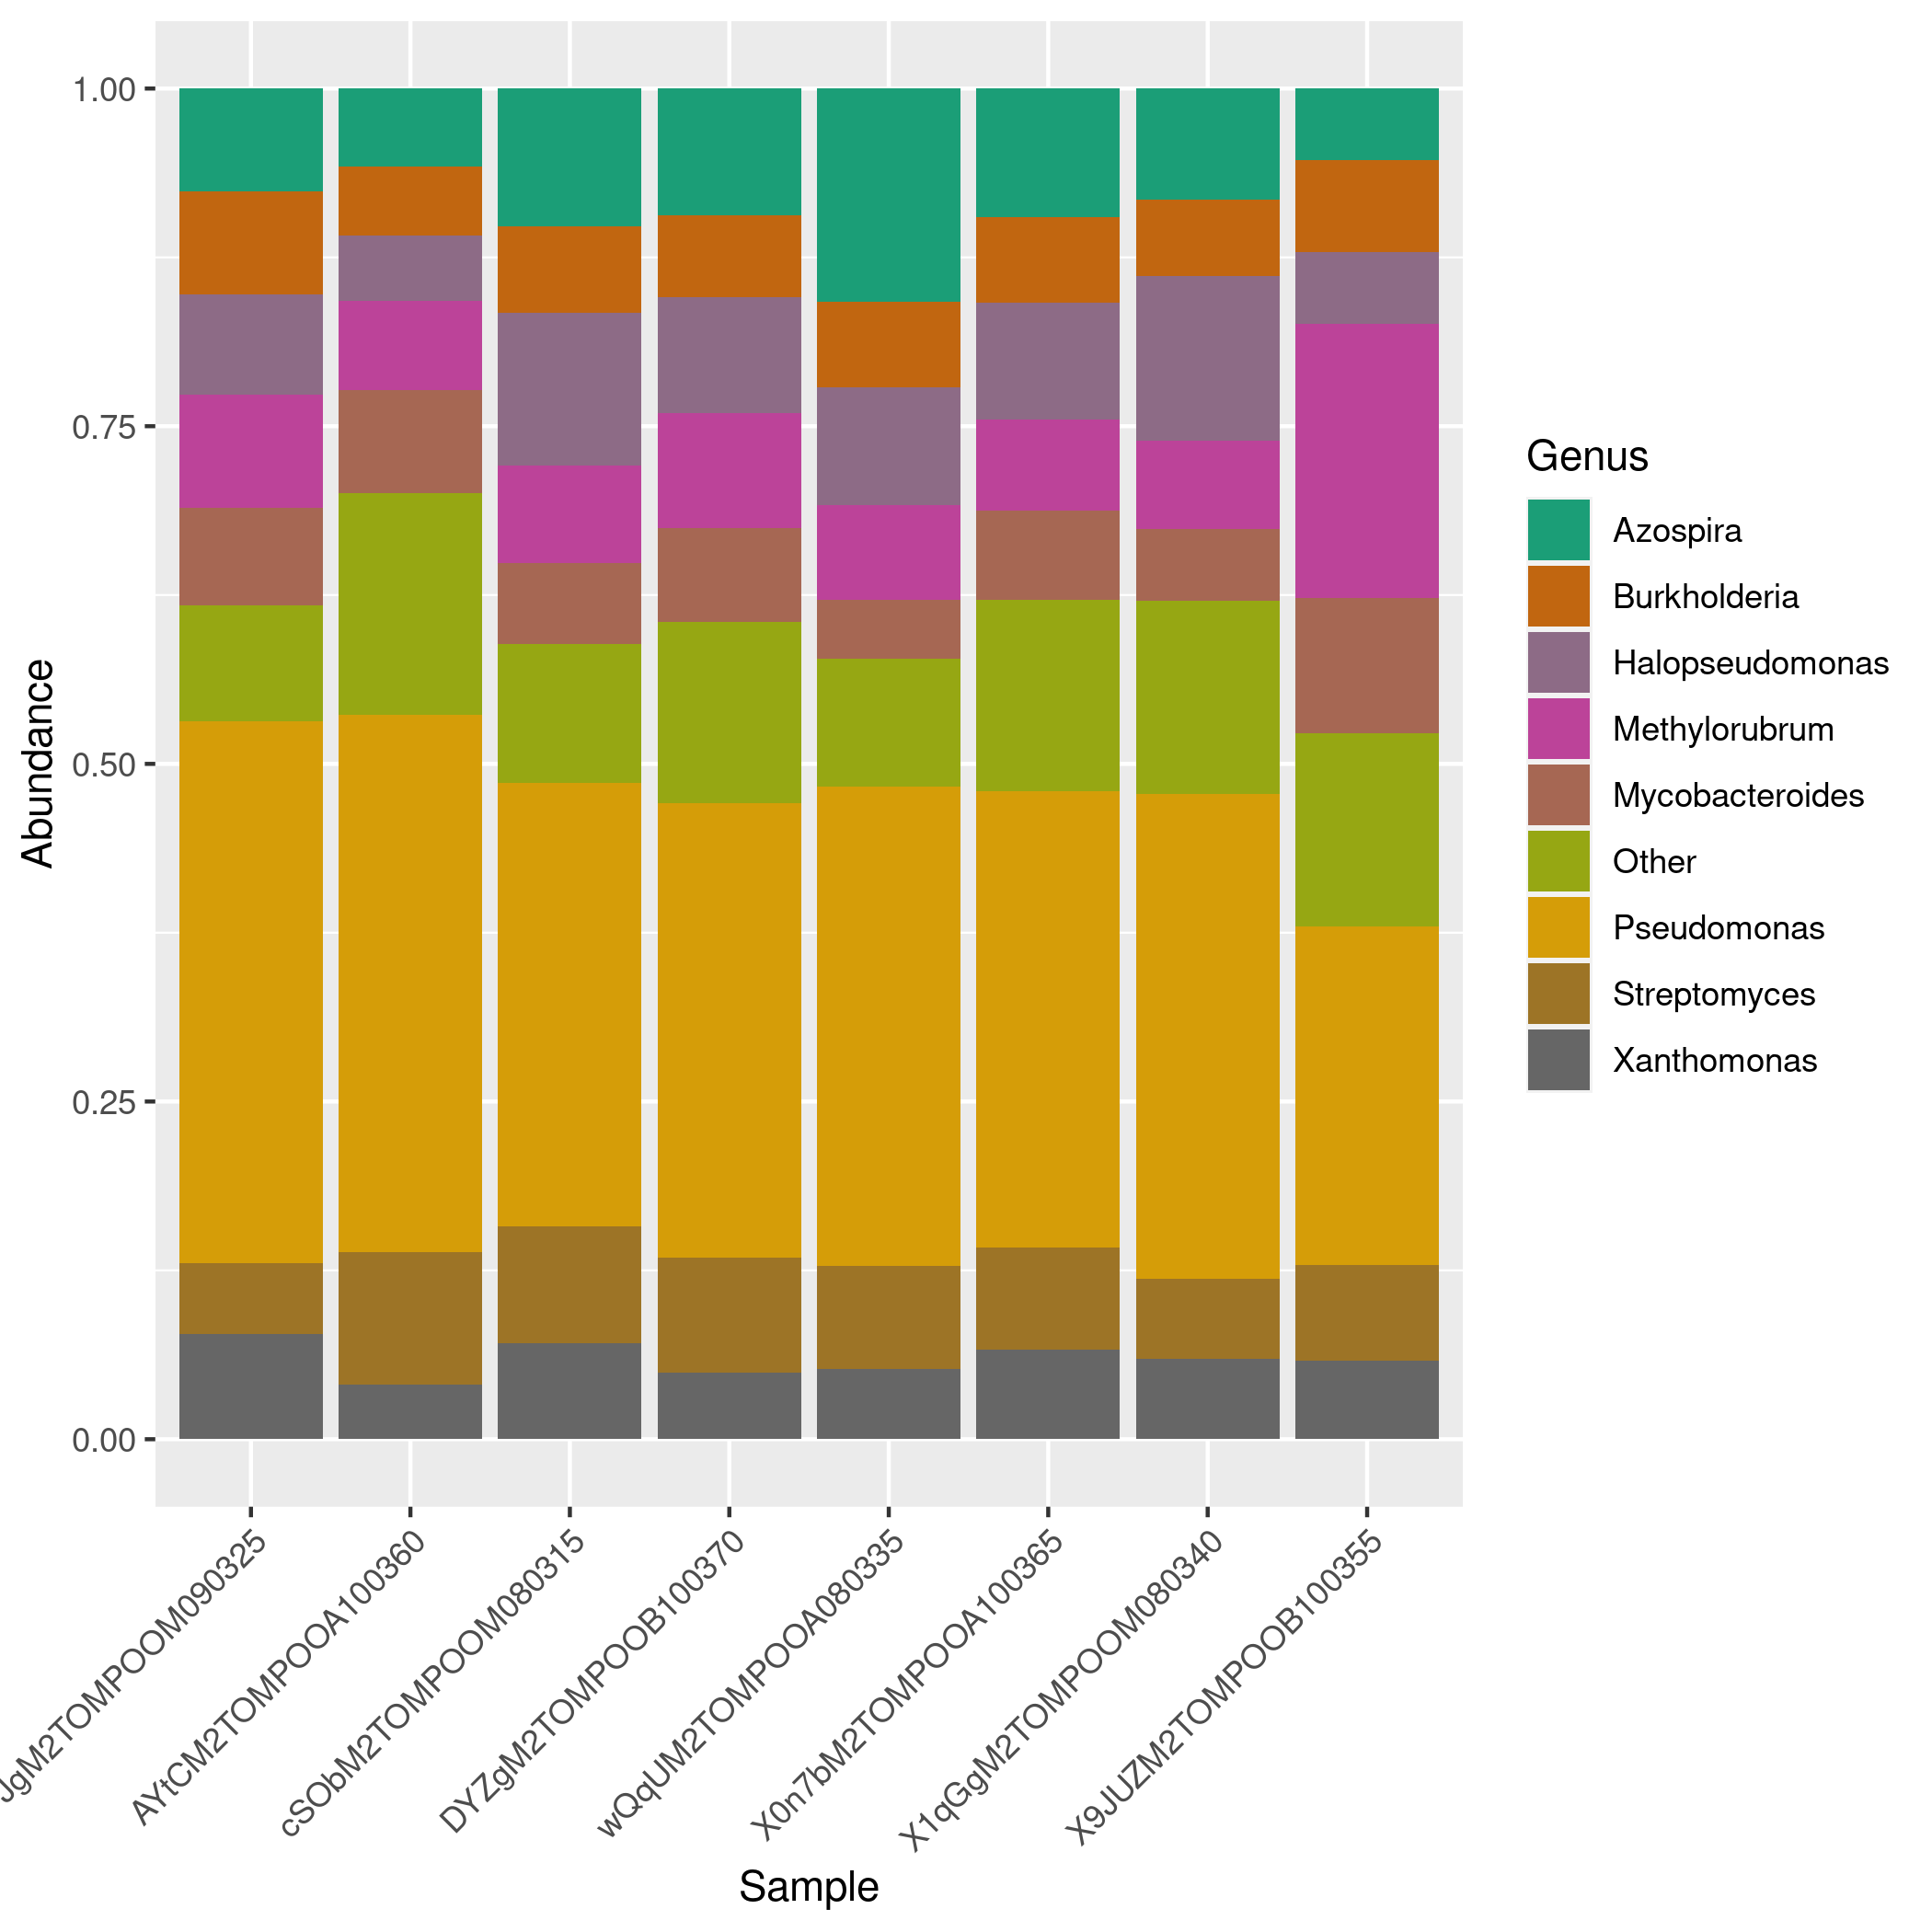
\includegraphics[scale = 0.8]{tomate_no_desarrollo.csv_relative_abundance_Genus.png}
    \caption{Relative abundance by genera of keystone OTUs in rhizosphere samples of \textit{Solanum lycopersicum} not labeled as ``Desarrollo".}
    \label{tomate_no_desarrollo_key_abundance_family}
\end{figure}

%\begin{figure}
%   \centering
%   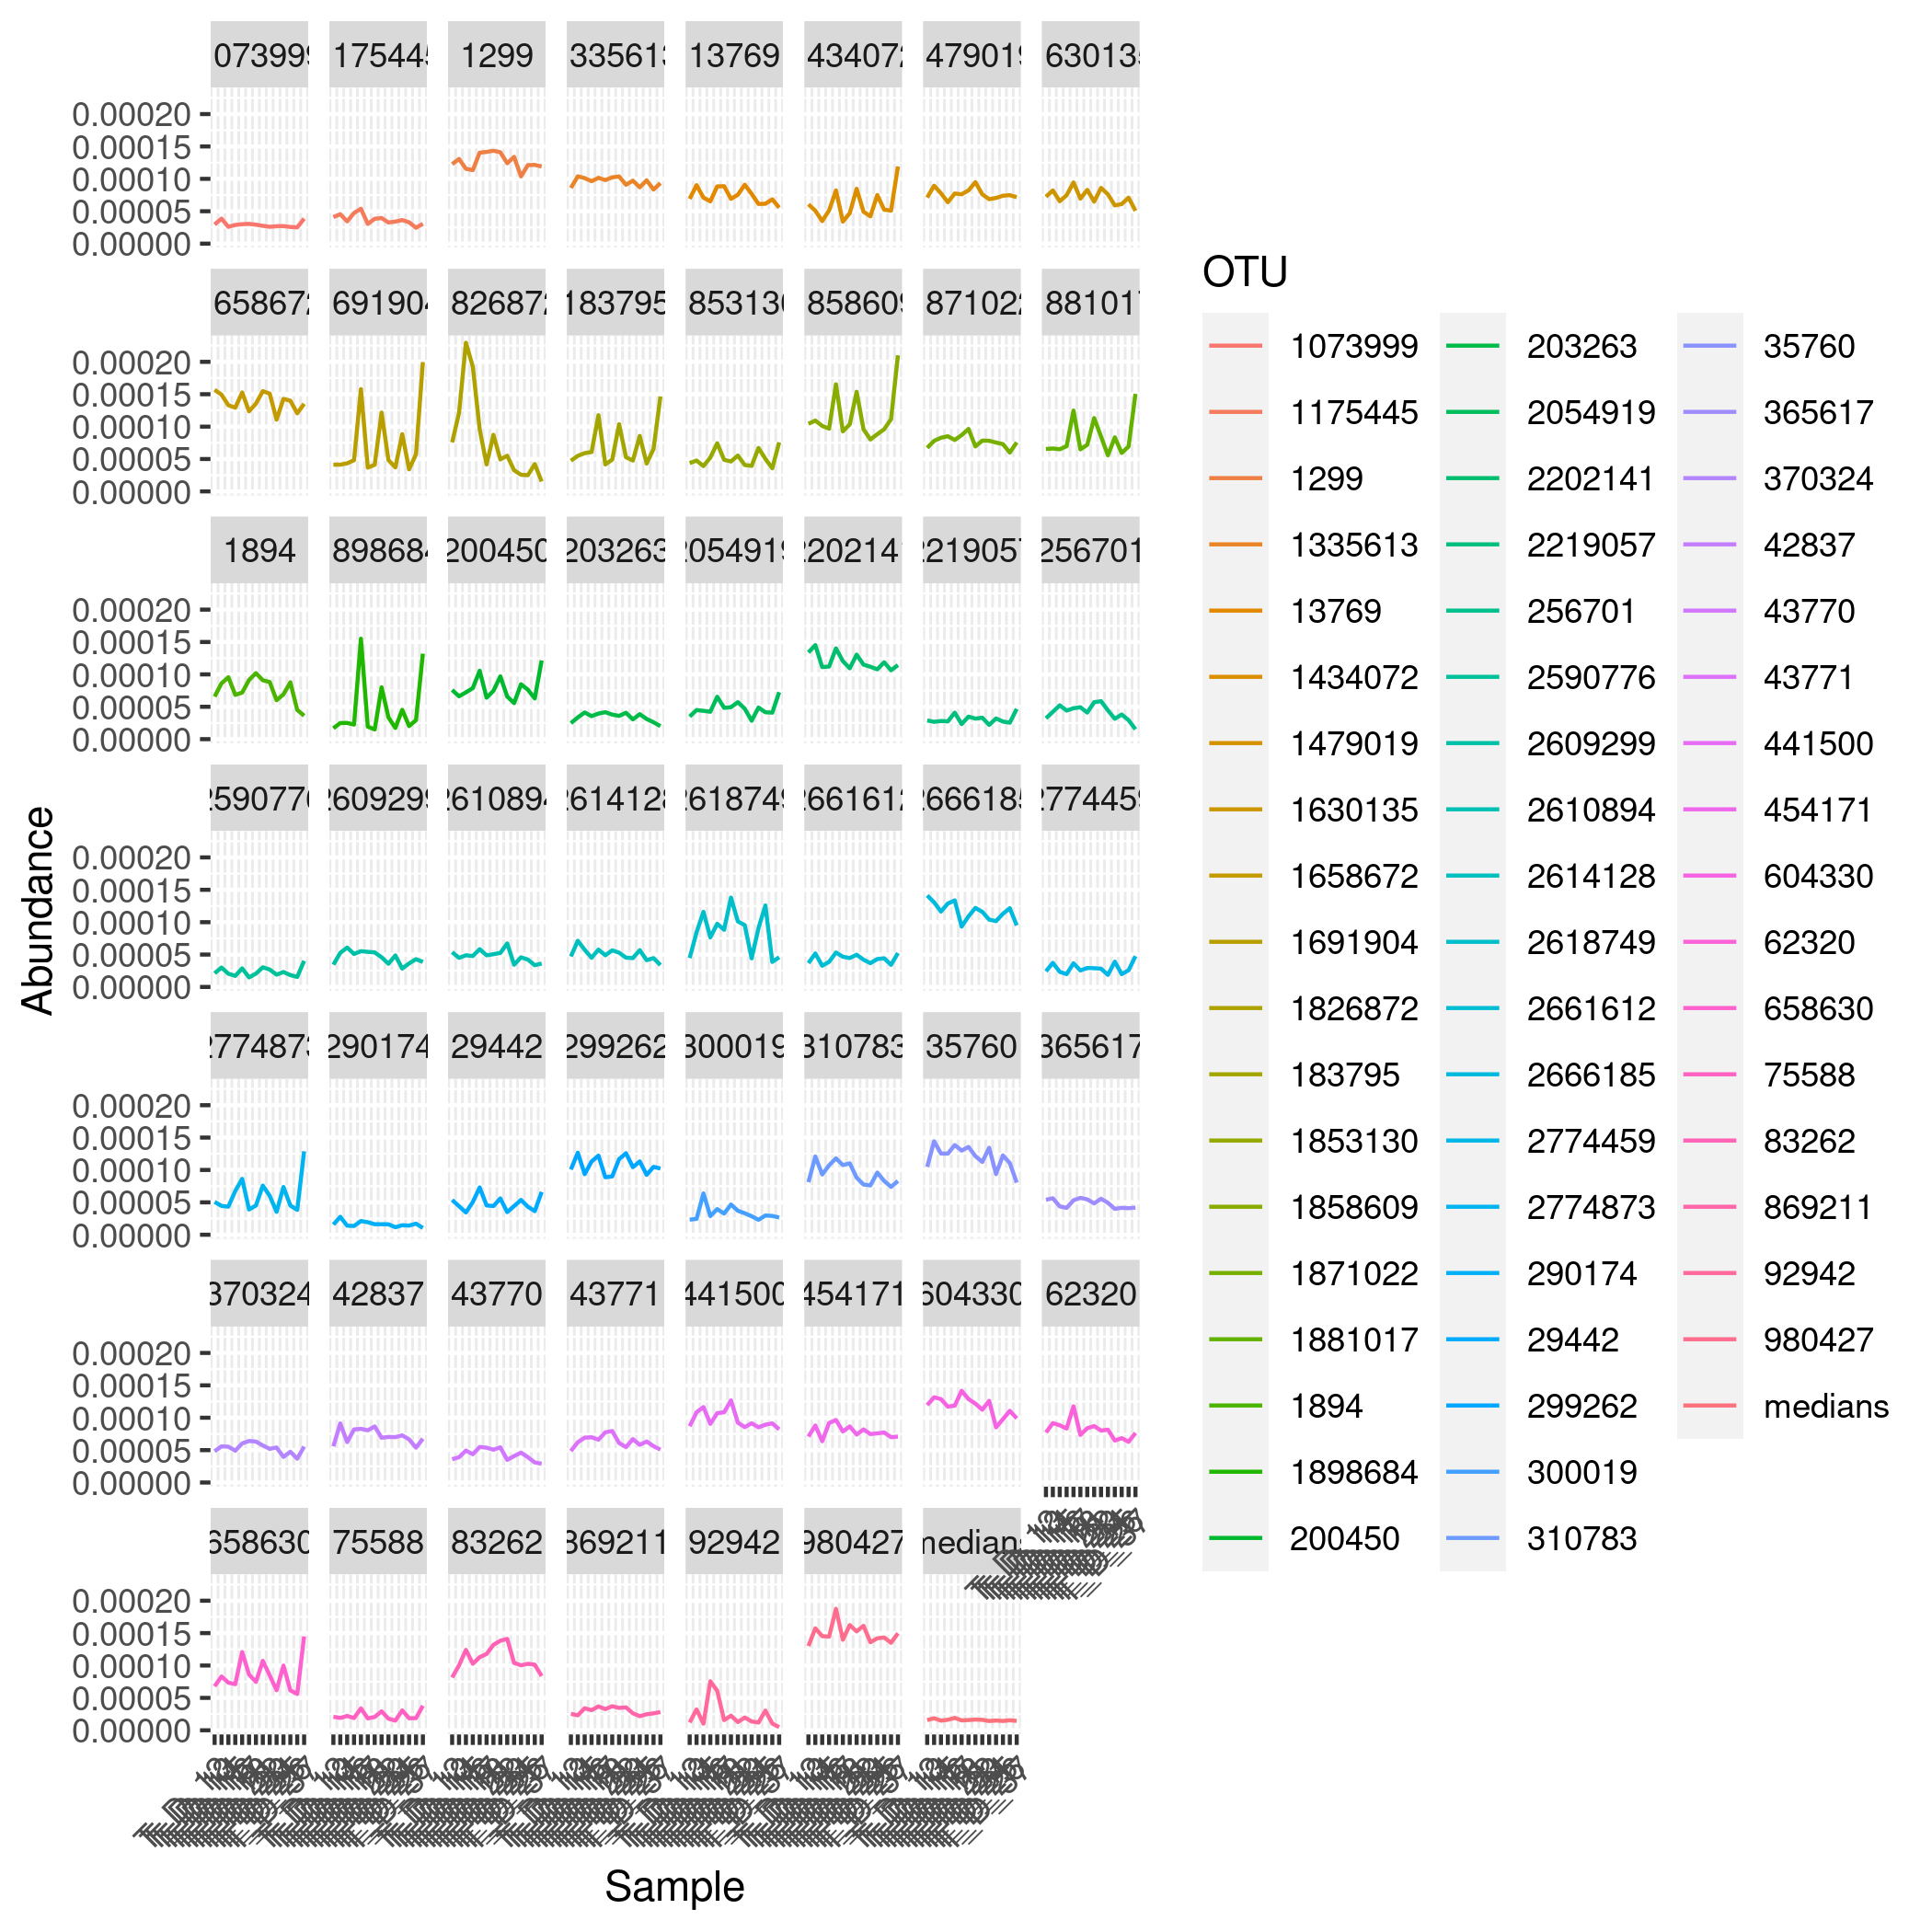
\includegraphics[scale = 0.8]{abundance_tomate_desarrollo.csv_key_otus_medians.png}
%   \caption{Plots representing relative abundance of each keystone OTU and one representing the median relative abundance  across samples of rhizosphere of tomate desarrollo. Most keystone OTUs have relative abundance bigger than the median across all samples.  }
%   \label{key_otus_vs_medians_tomate_desarrollo.csv}
%\end{figure}

%\begin{figure}
%   \centering
%   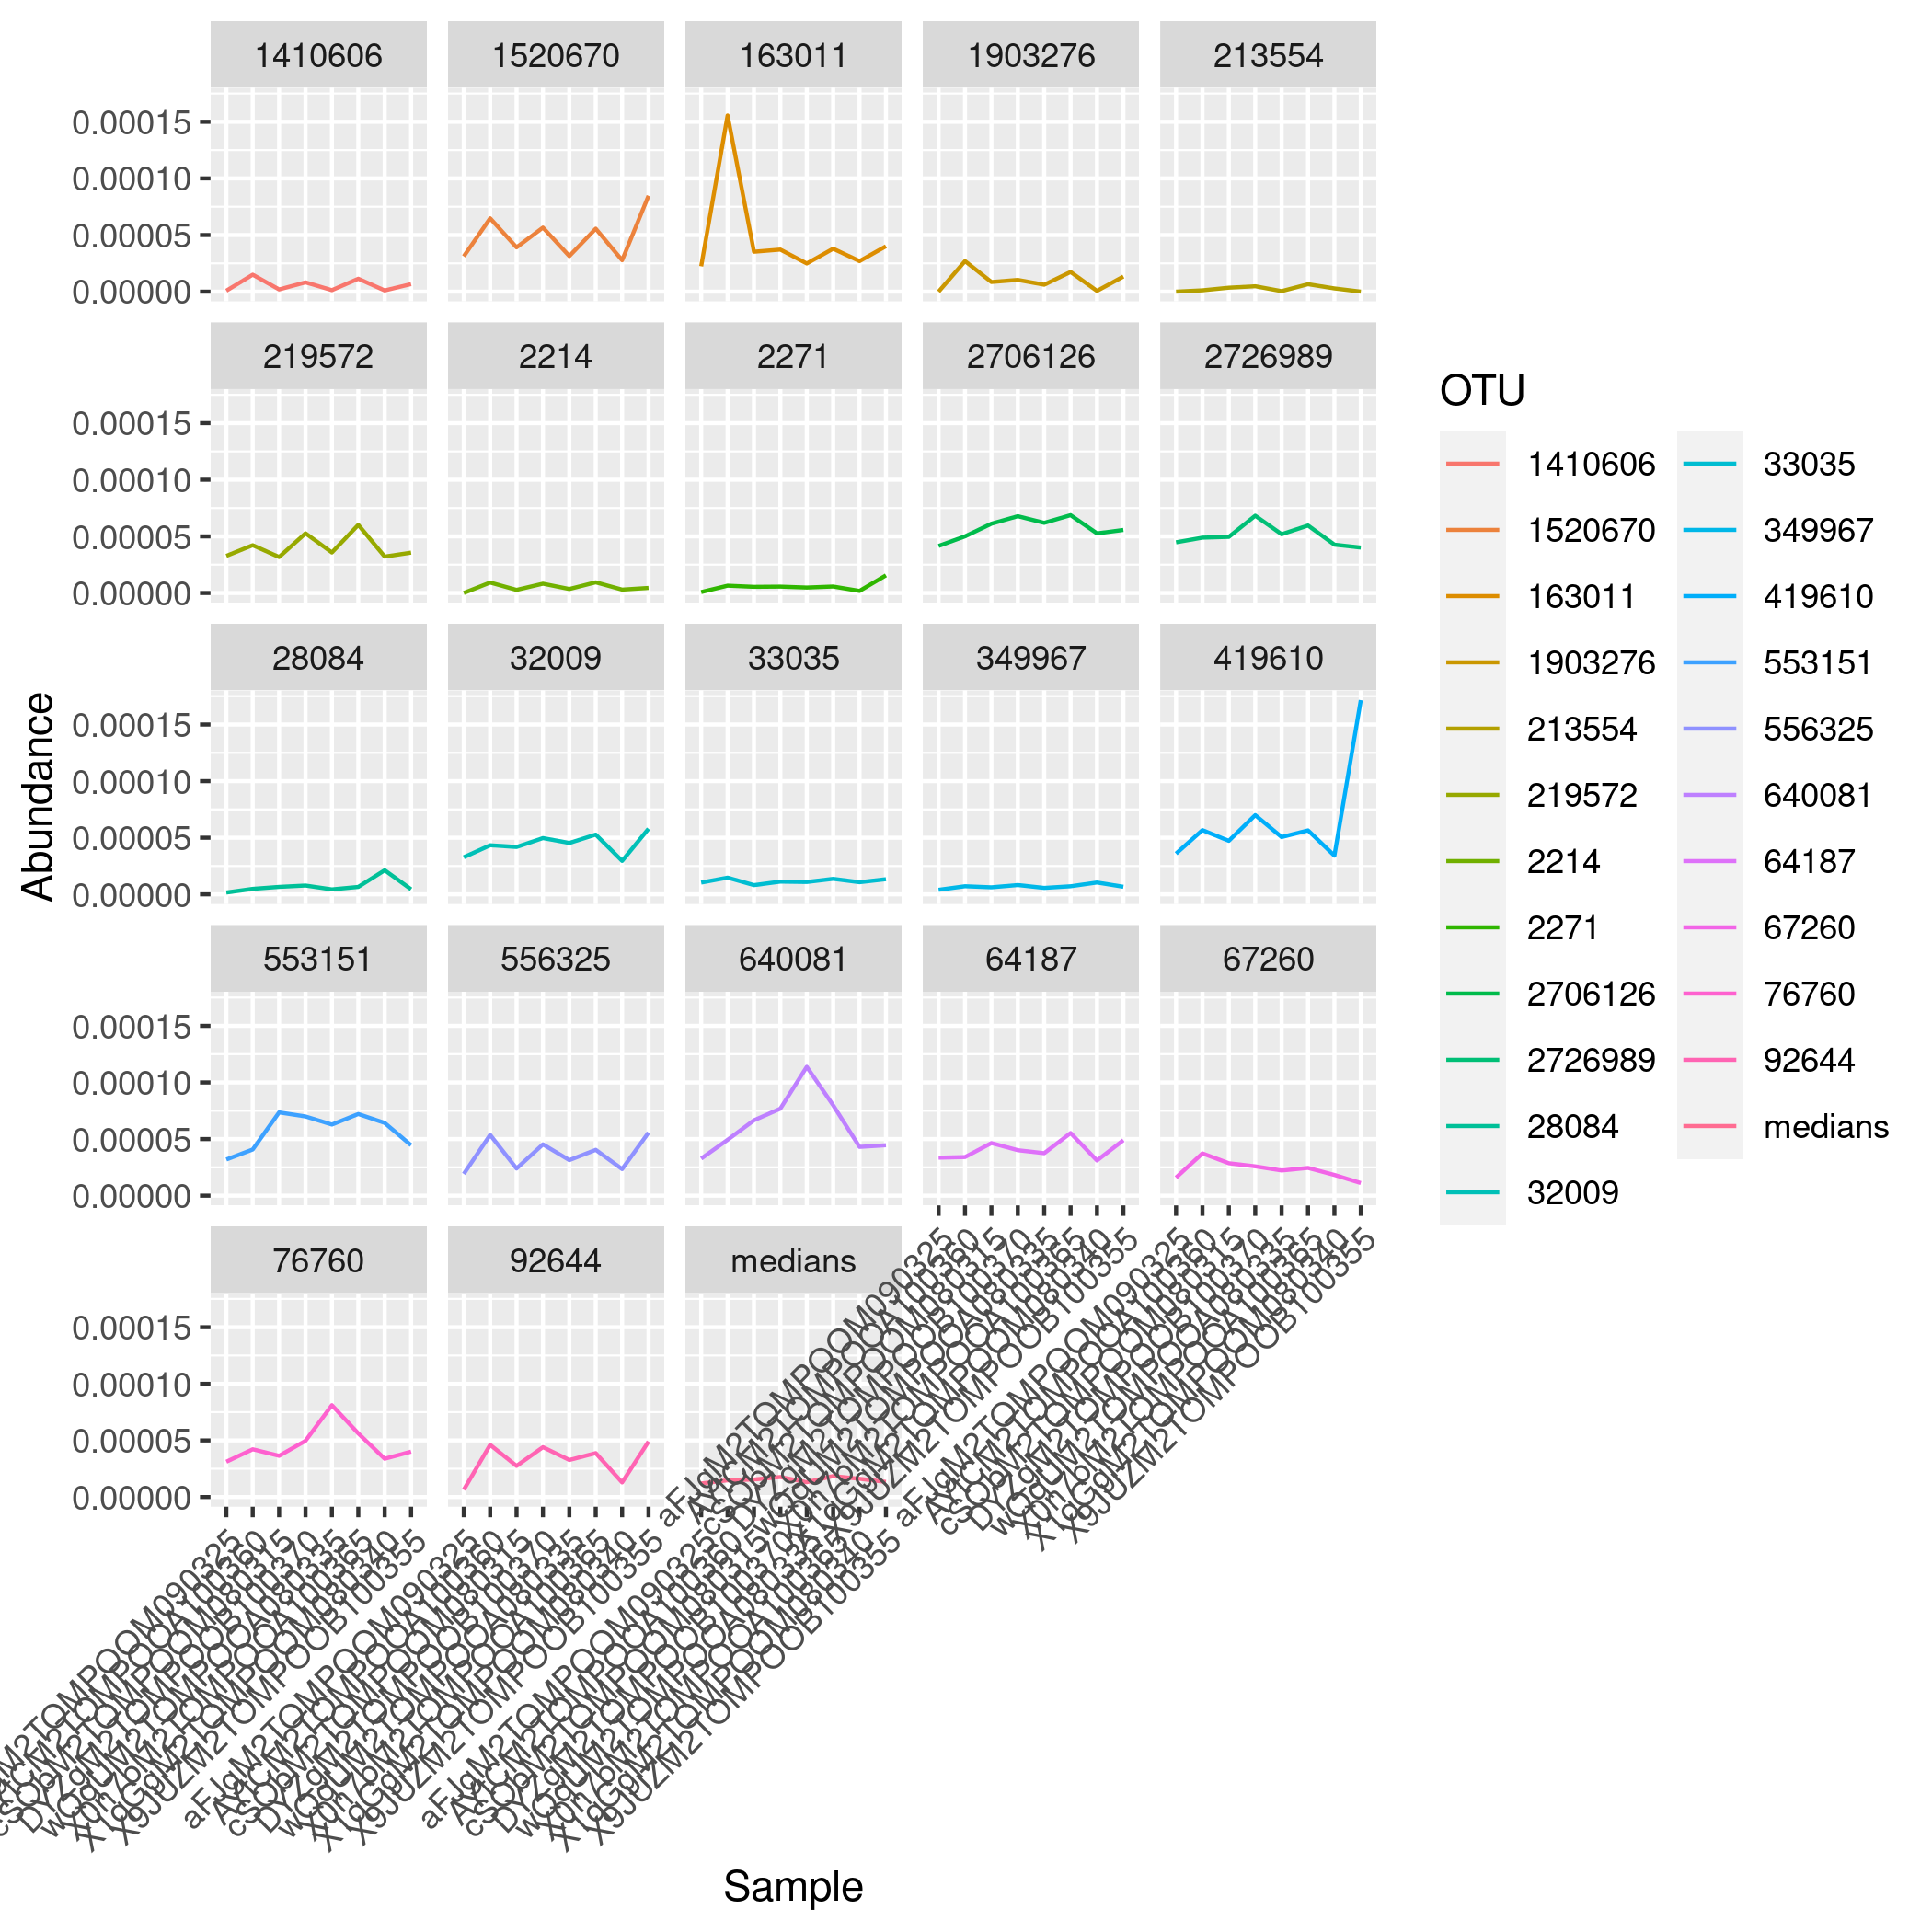
\includegraphics[scale = 0.8]{abundance_tomate_no_desarrollo.csv_key_otus_medians.png}
%   \caption{Plots representing relative abundance of each keystone OTU and one representing the median relative abundance  across samples of rhizosphere of tomate no desarrollo.csv. Most keystone OTUs have relative abundance bigger than the median across all samples.  }
%   \label{key_otus_vs_medians_tomate_no_desarrollo.csv}
%\end{figure}



%distribuciones otus clave vs muestras 
\begin{figure}
 \centering
 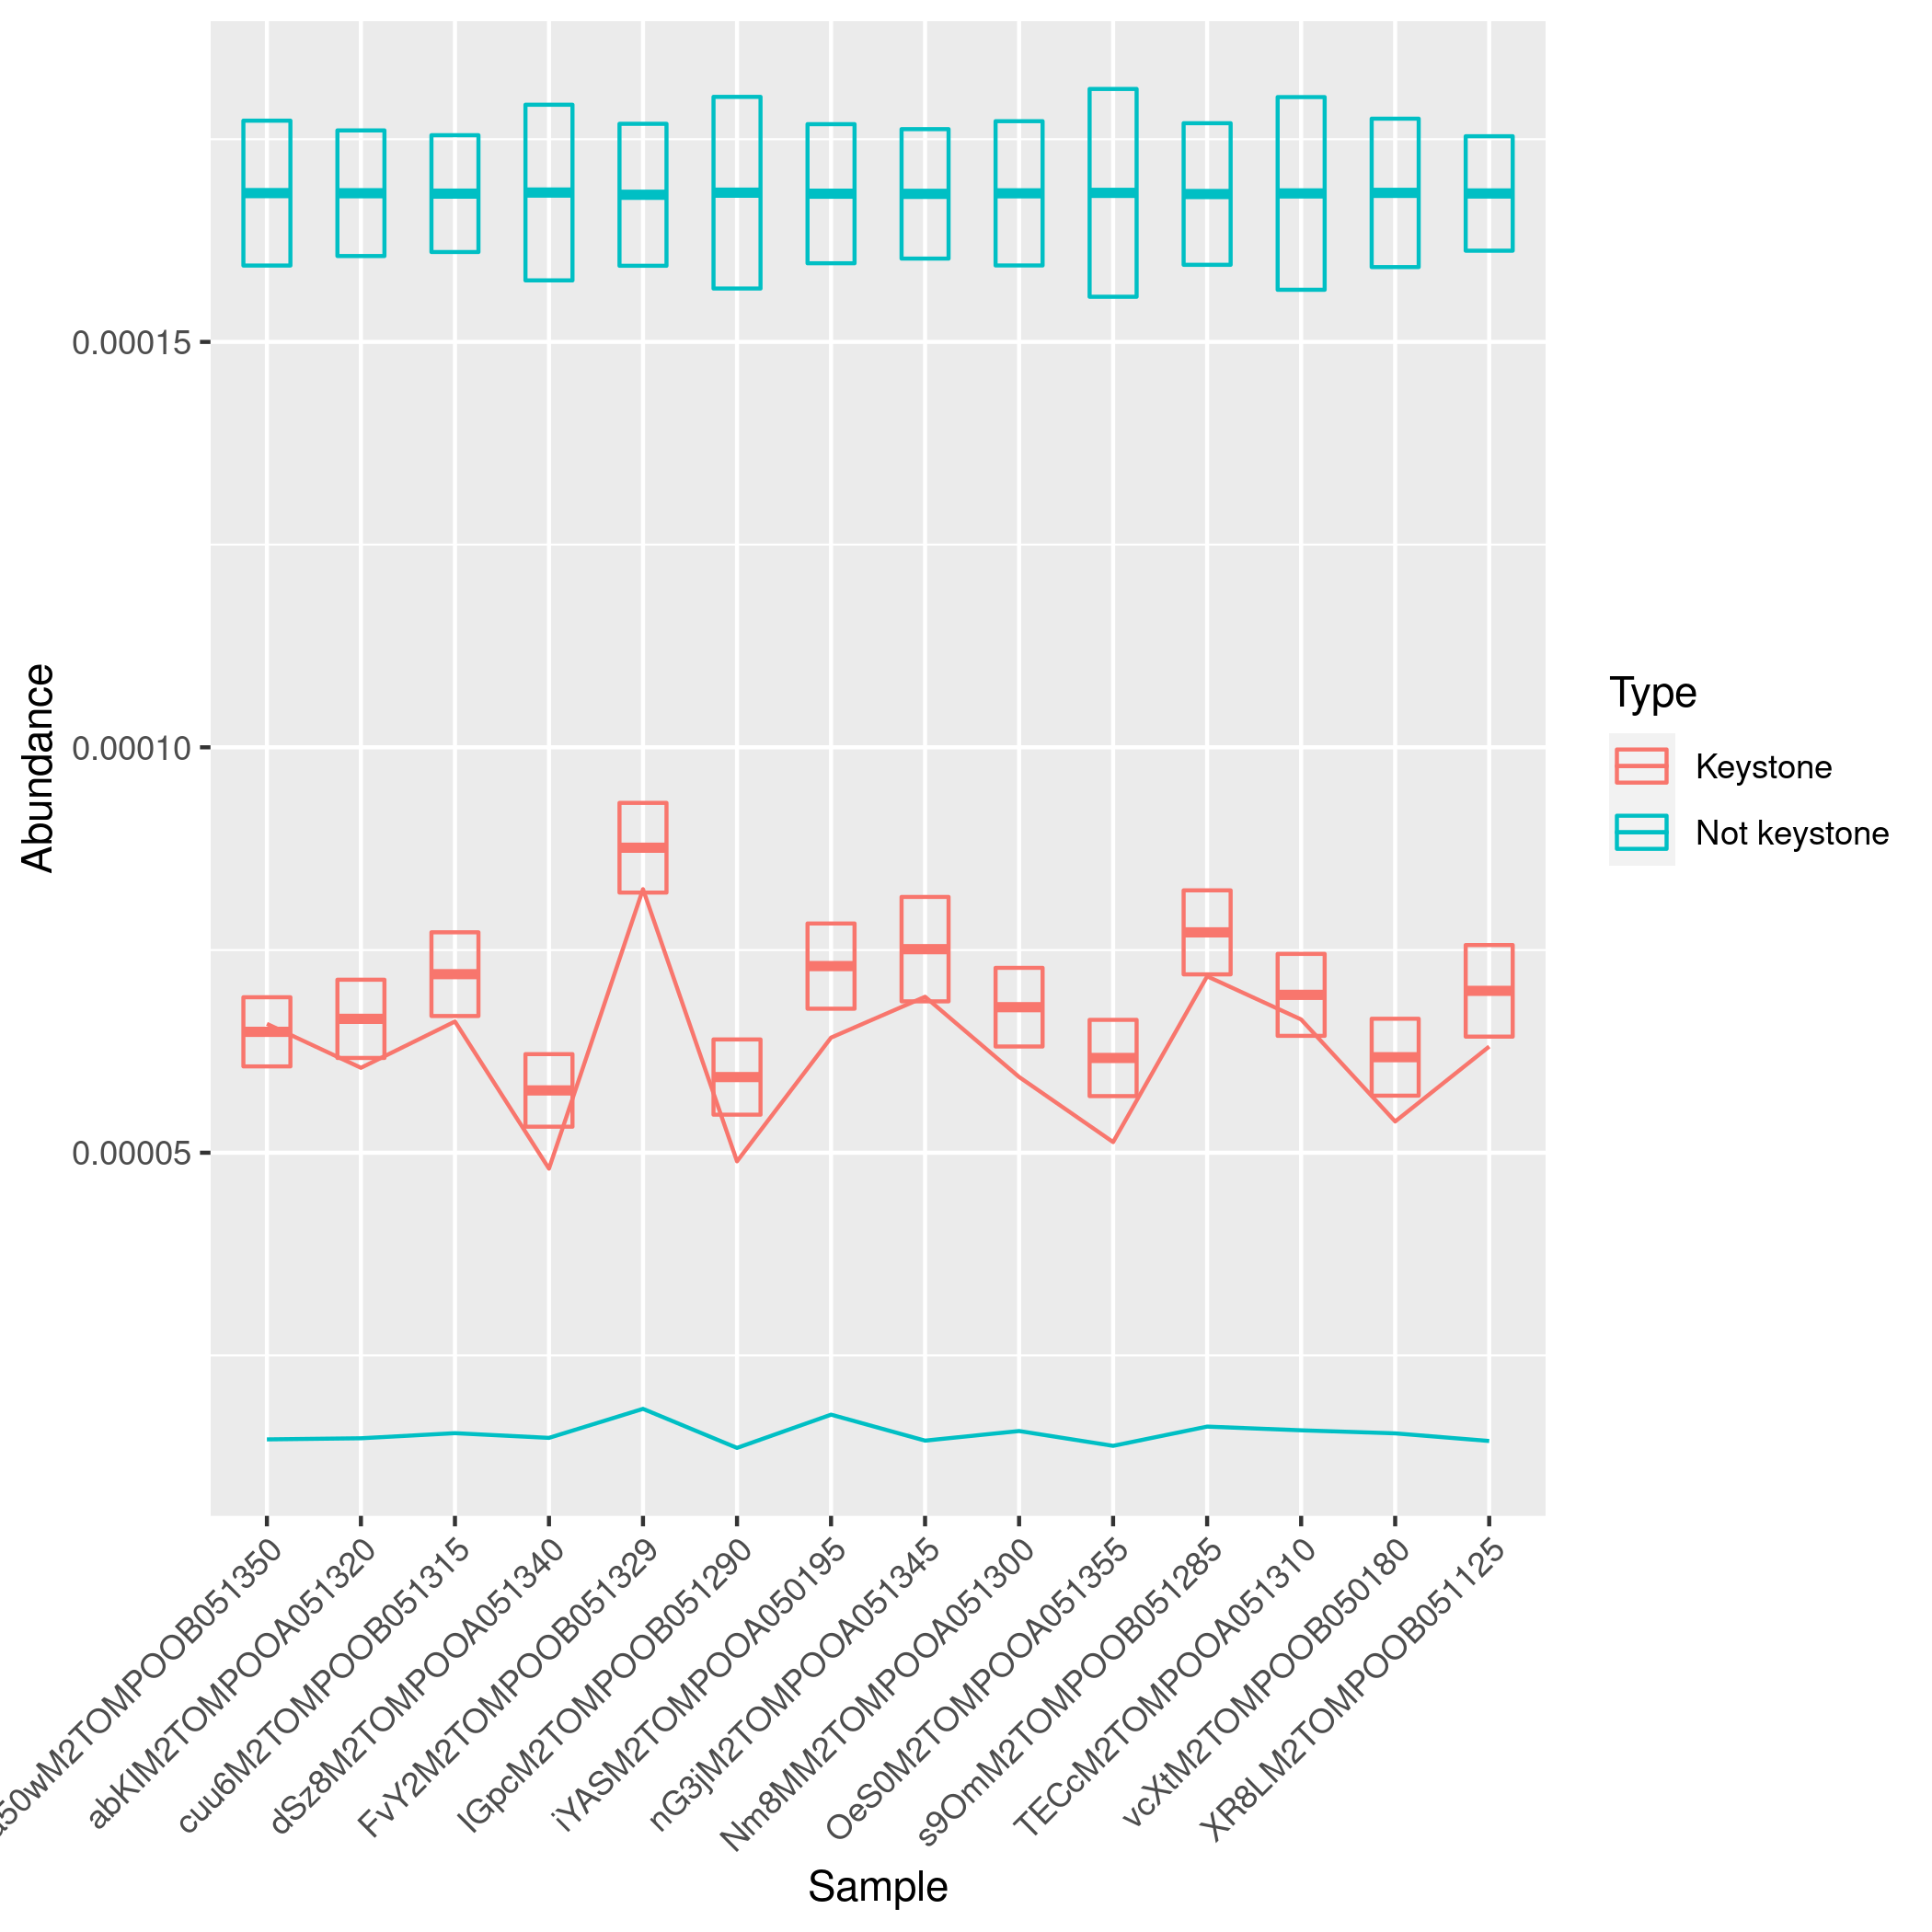
\includegraphics[scale = 0.75]{mean_median_key_vs_not_key_tomate_desarrollo.csv.png}
\caption{Boxes represent mean and standard error in the distribution of corresponding samples.} %Lines represent the corresponding medians. In these samples of rhizosphere oftomate_desarrollo.csv}
\label{mean_median_tomate_desarrollo.csv}
\end{figure}

\begin{figure}
 \centering
 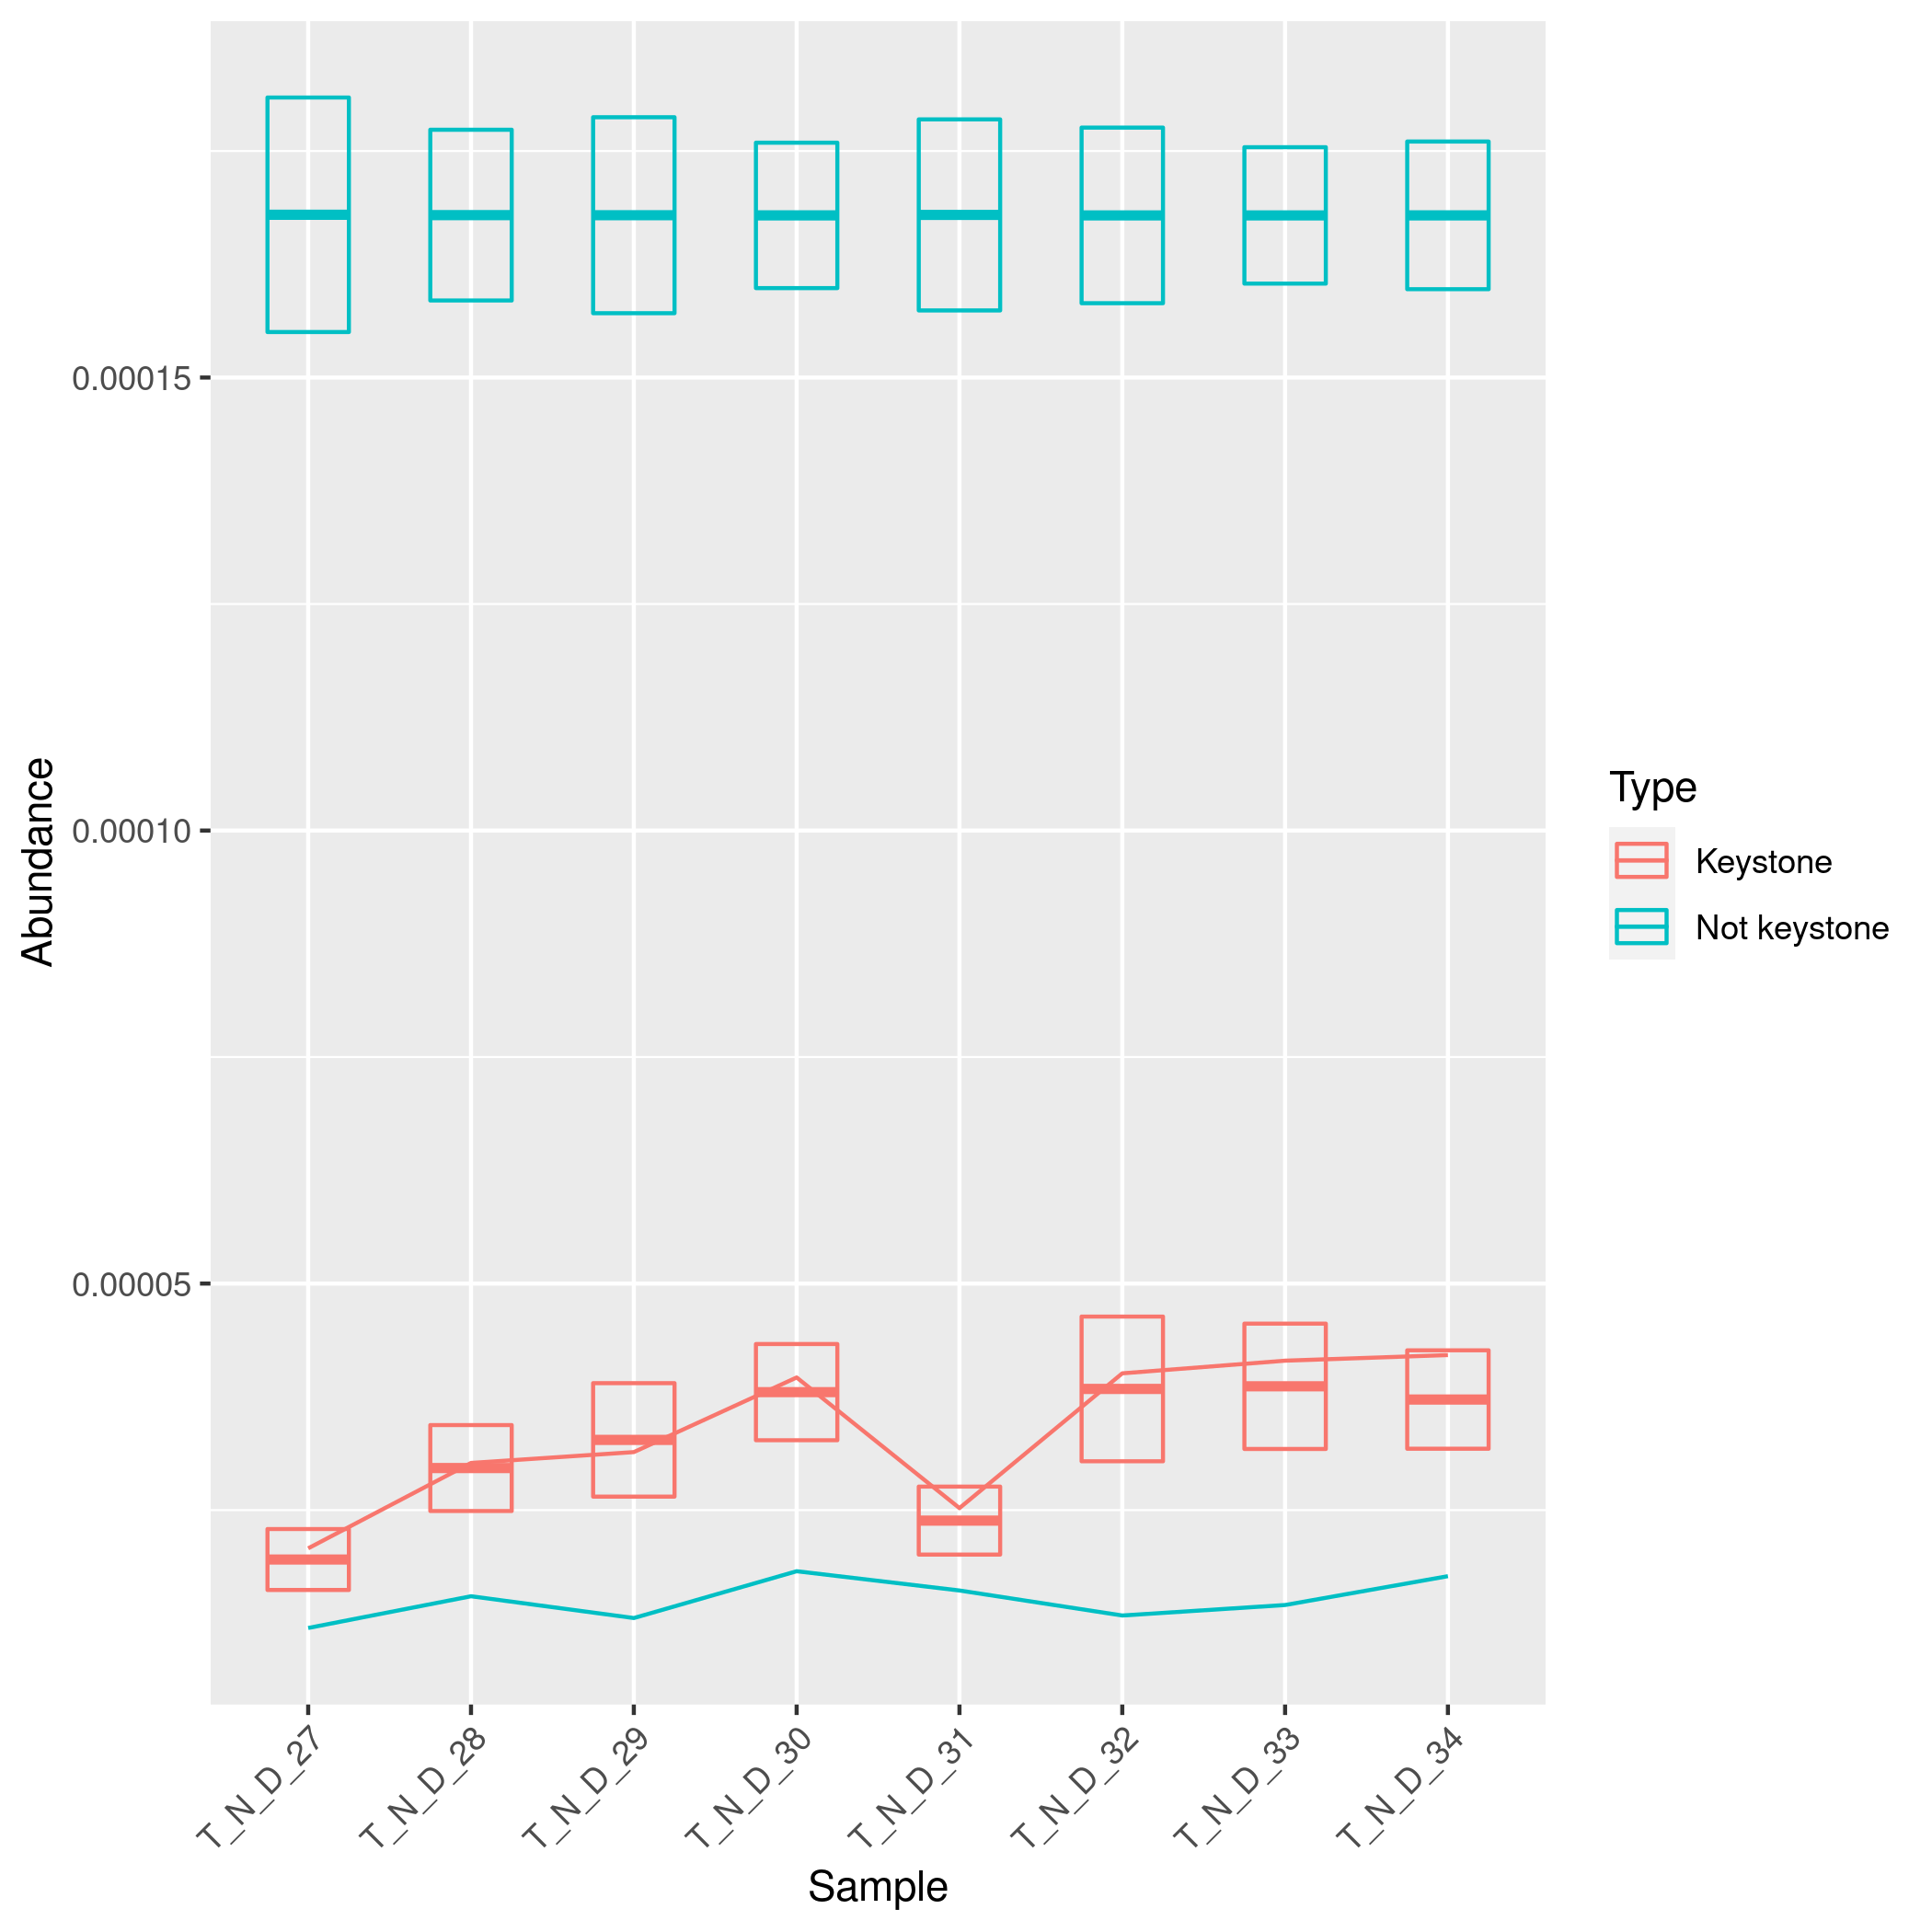
\includegraphics[scale = 0.75]{mean_median_key_vs_not_key_tomate_no_desarrollo.csv.png}
\caption{Boxes represent mean and standard error in the distribution of corresponding samples. Lines represent the corresponding medians. In these samples of rhizosphere oftomate no desarrollo.csv}
\label{mean_median_tomate_no_desarrollo.csv}
\end{figure}

\begin{figure}
    \centering
    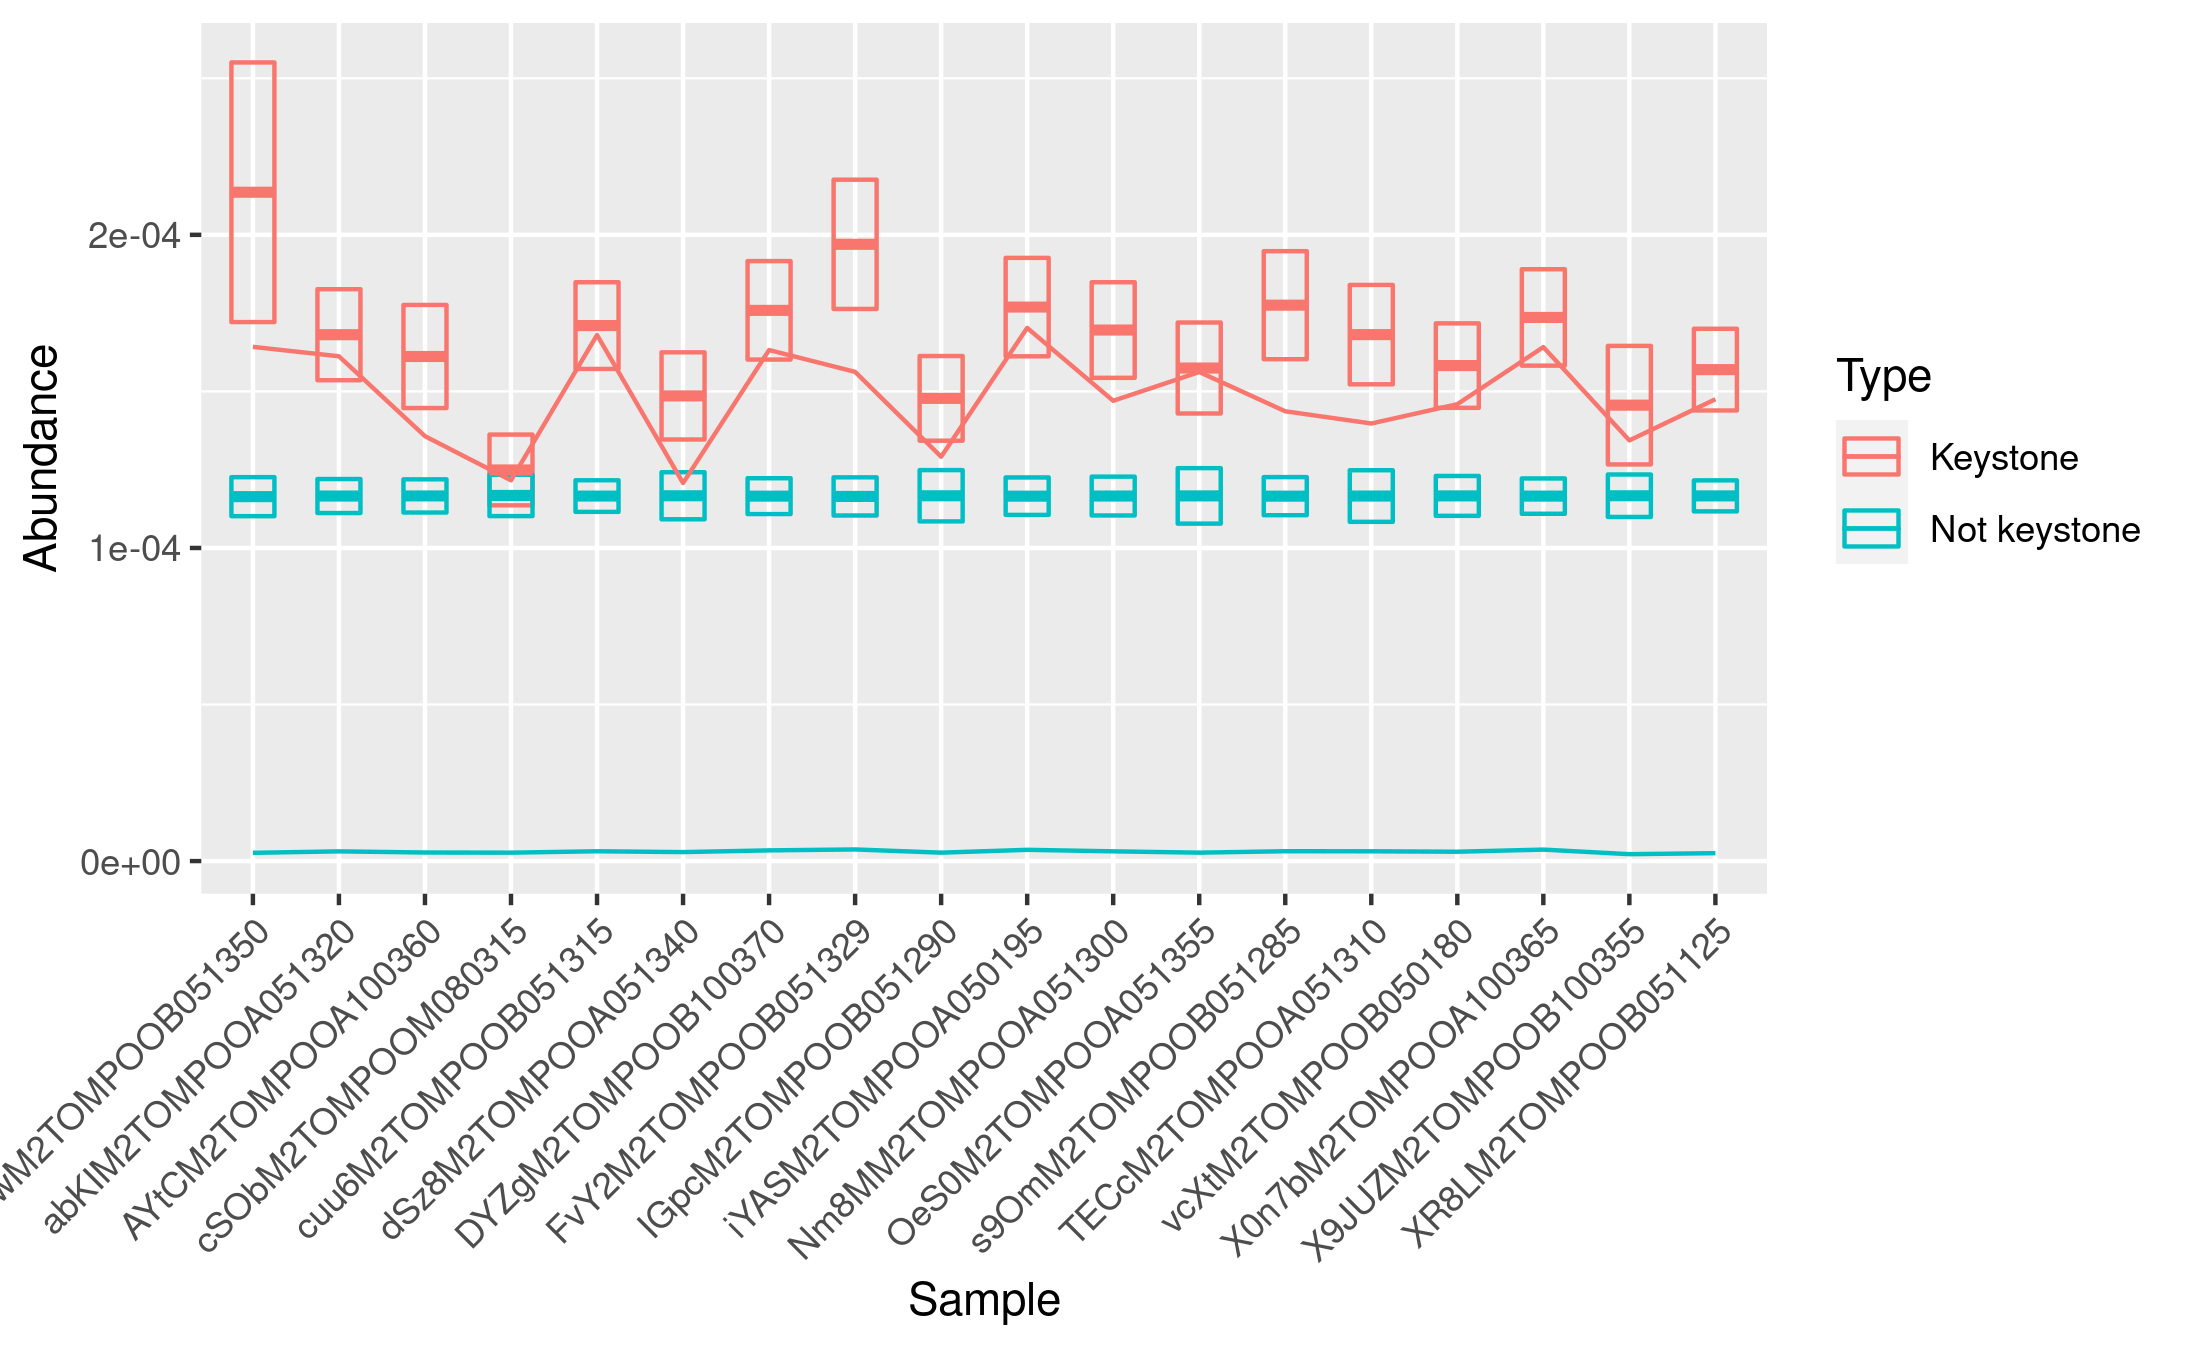
\includegraphics[scale = 0.75]{mean_median_key_vs_not_key_tomate.png}
    \caption{Boxes represent mean and standard error in the distribution of corresponding samples. Lines represent the corresponding medians. In these samples of rhizosphere of \textit{Solanum lycopersicum} relative abundance keystone OTUs tend to be higher than the median and the mean of the relative abundance of all other OTUs. }
    \label{mean_median_tomate}
\end{figure}

%analisis pcoa
\begin{figure}
   \centering
   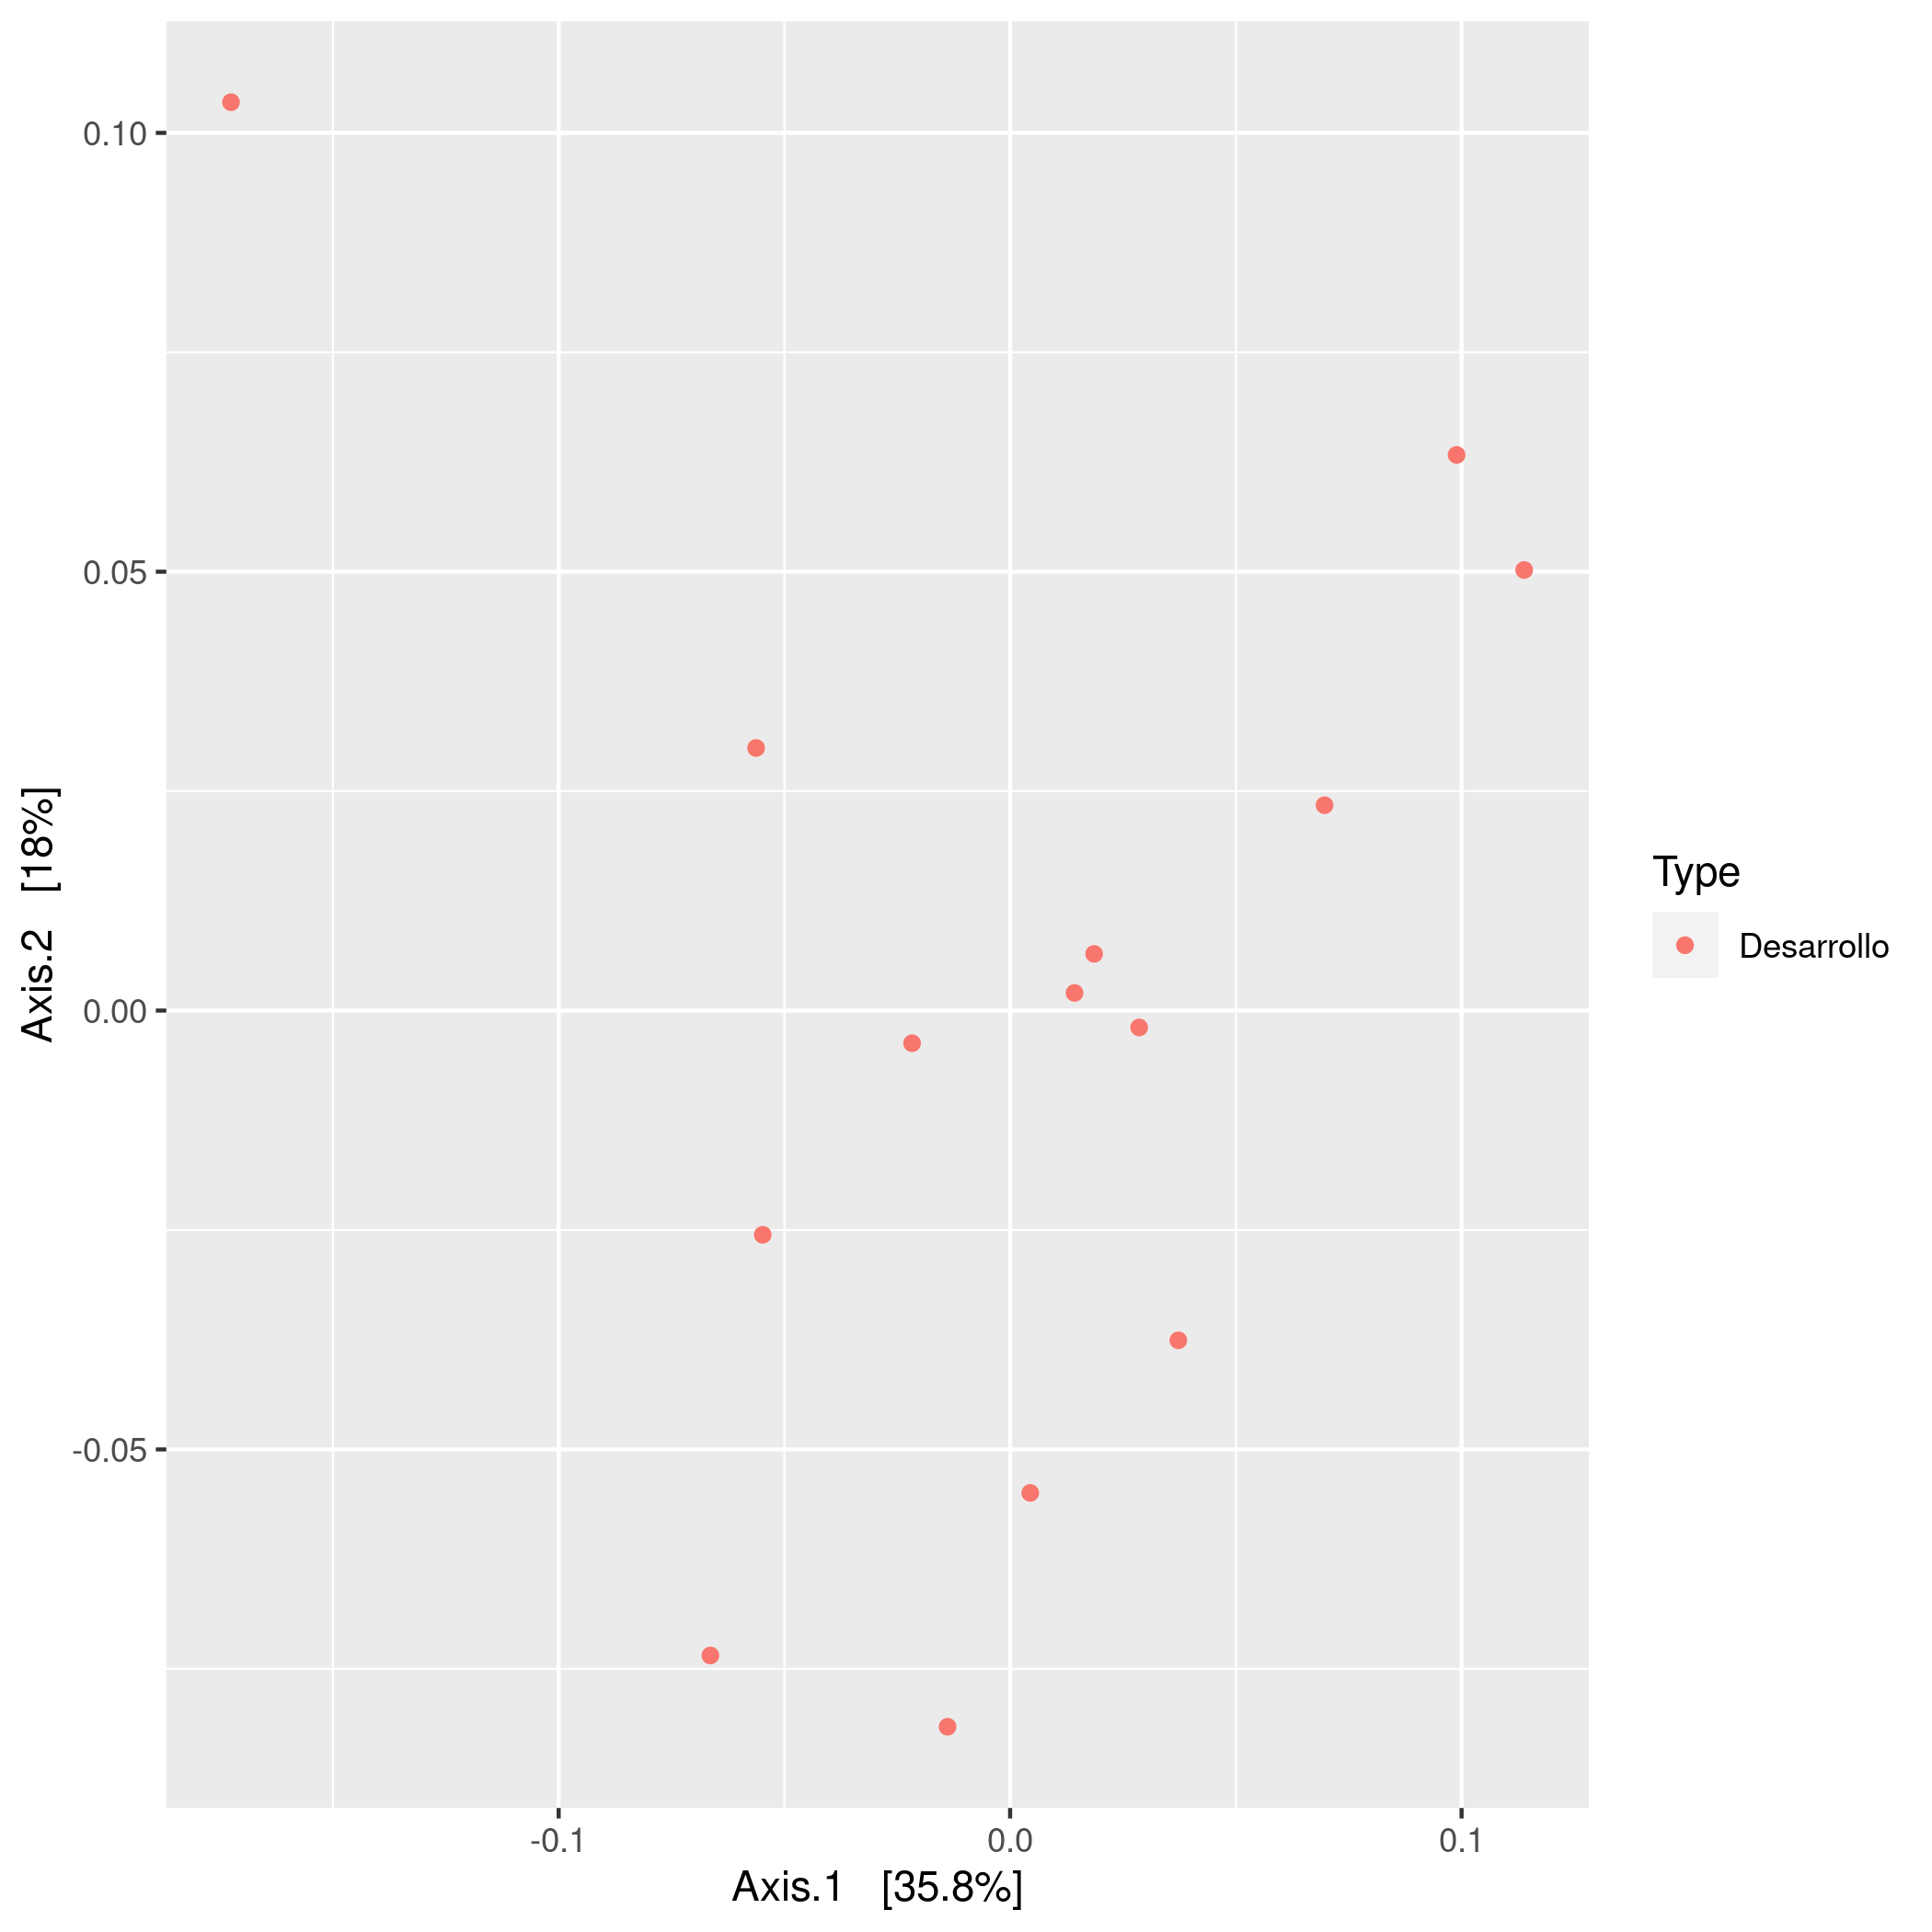
\includegraphics[scale = 0.7]{pcoa_muestras_tomate_desarrollo.csv.png}
 \caption{PCoA analysis with Bray-Curtis distance of rhizosphere samples }%of tomate_desarrollo.csv.}
 \label{fig:tomate_desarrollo.csv_pcoa}
\end{figure}
\begin{figure}
  \centering
  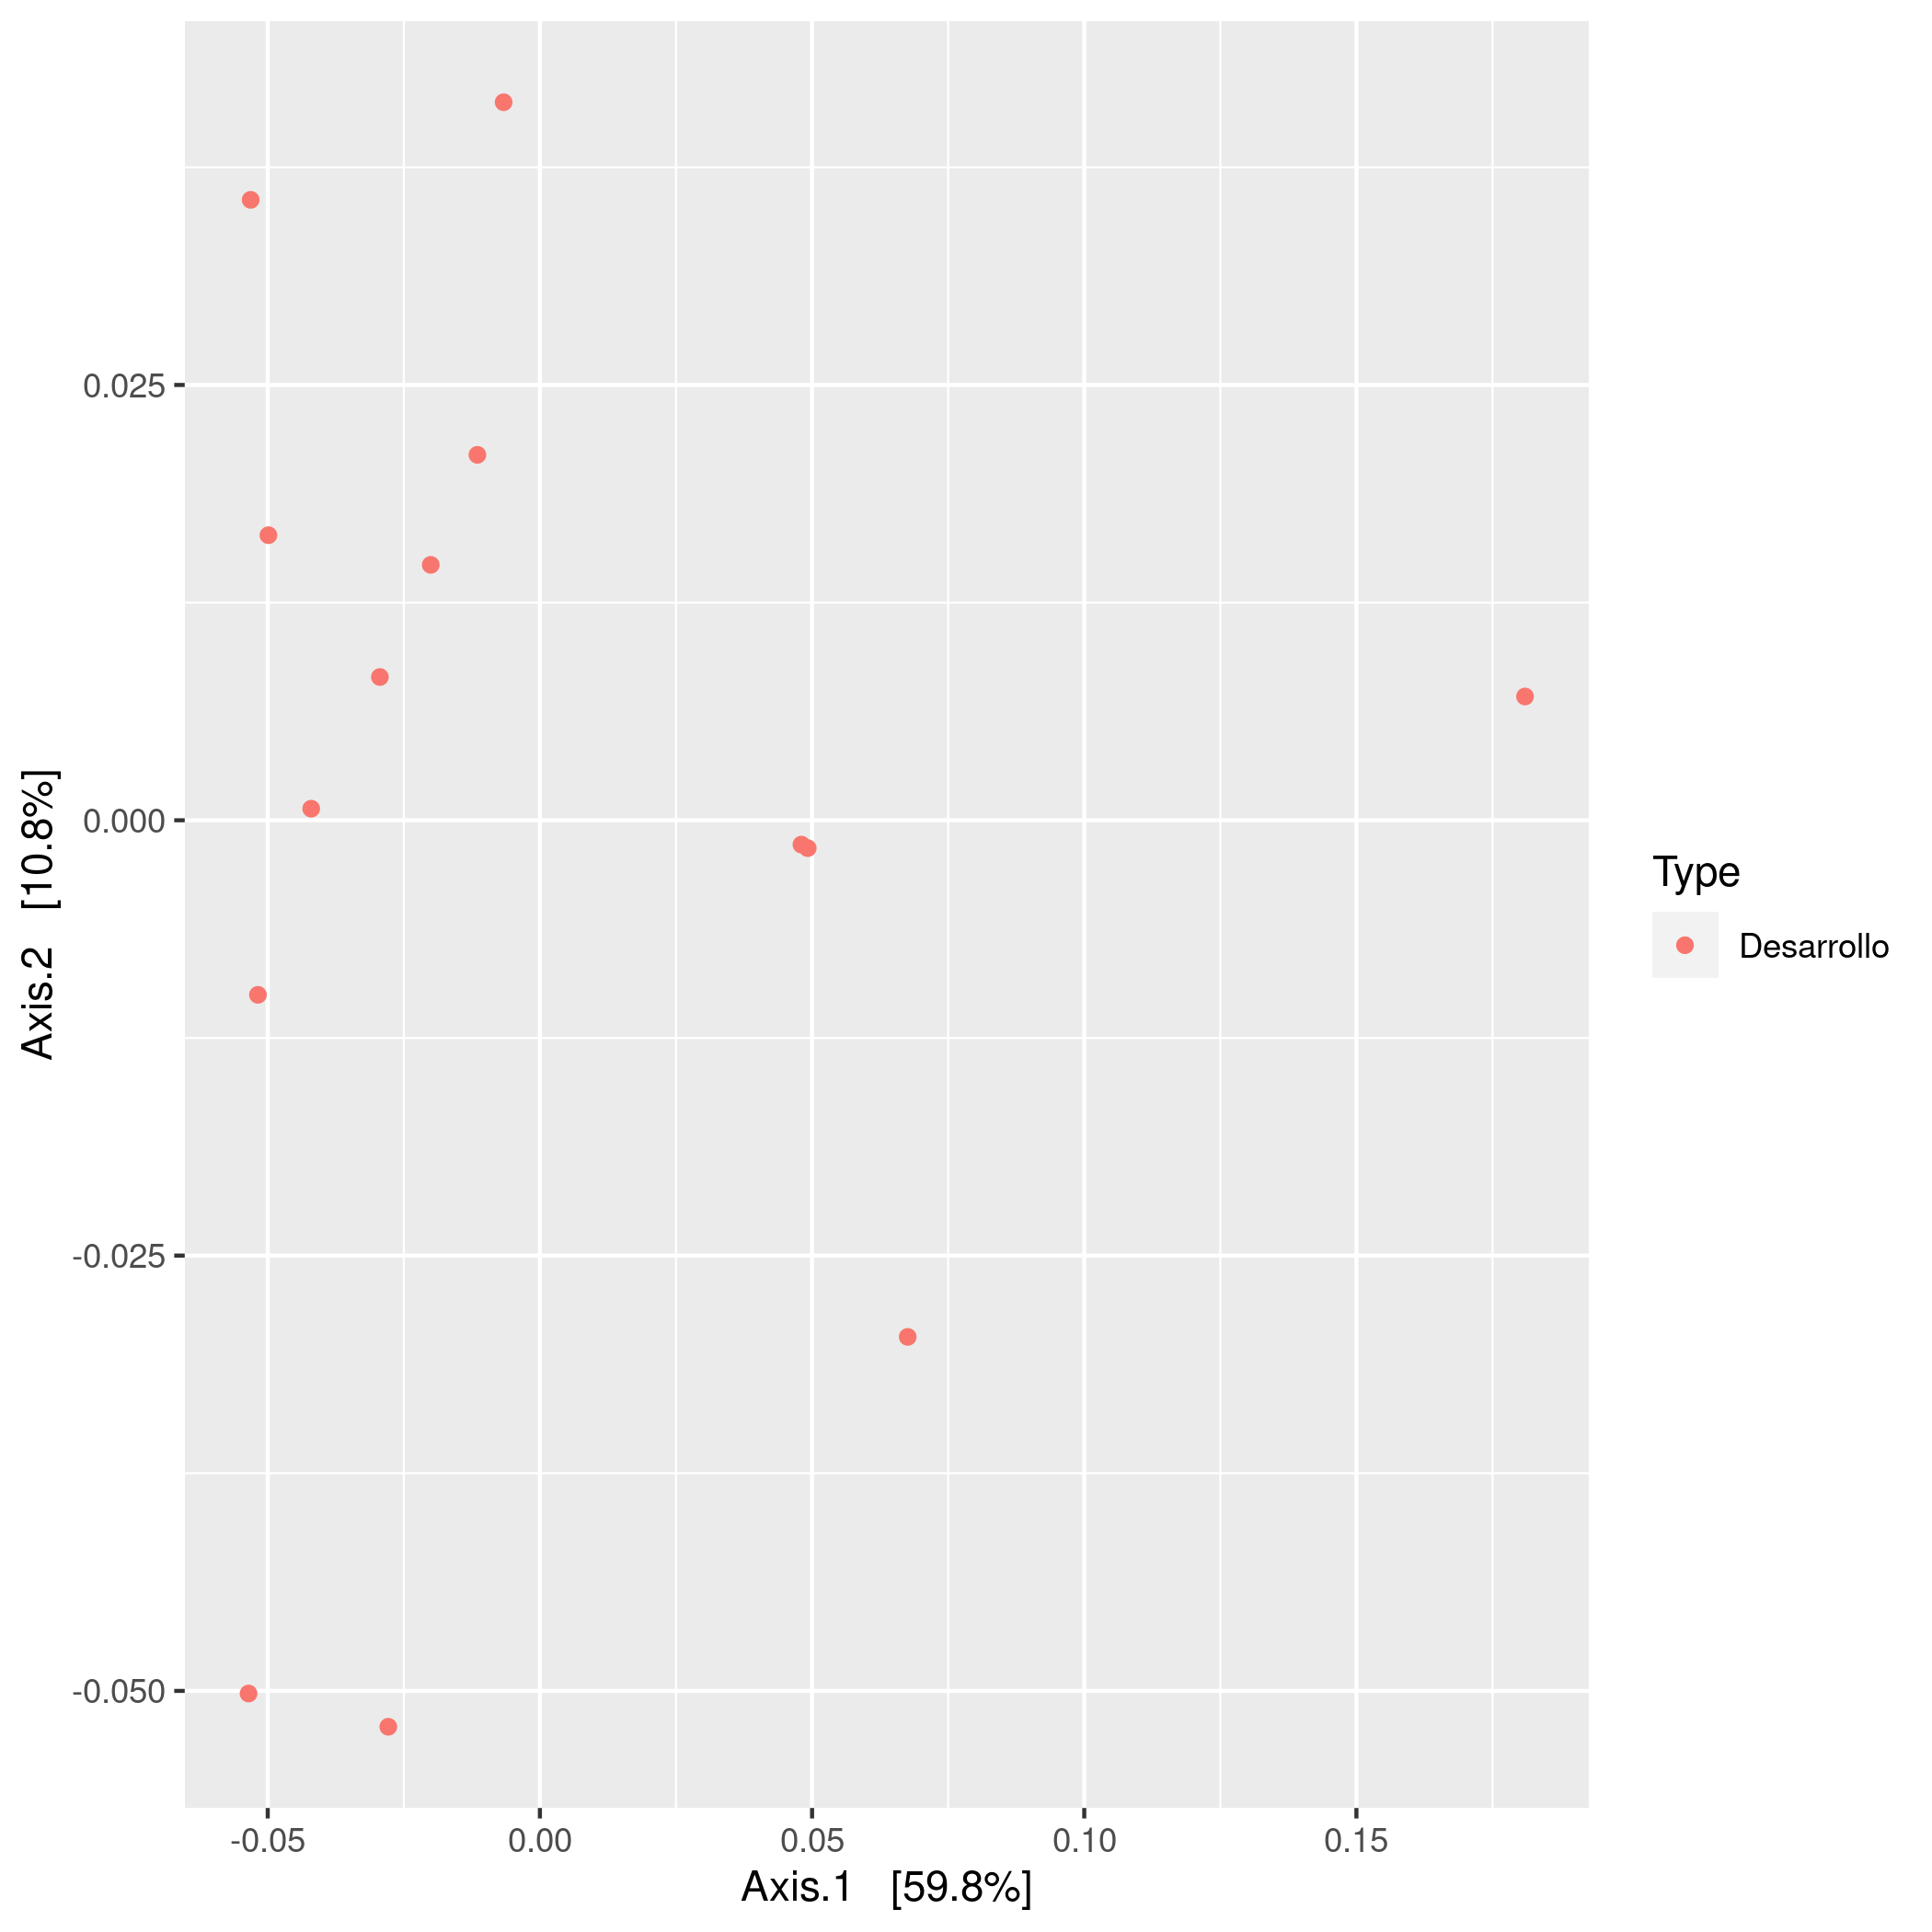
\includegraphics[scale = 0.7]{pcoa_key_otus_tomate_desarrollo.csv.png}
  \caption{PCoA analysis with Bray-Curtis distance of rhizosphere samples }%`of tomate_desarrollo.csv, restricted to keystone OTUs.}
  \label{fig:tomate_desarrollo.csv_pcoa_key_otus}
\end{figure}





\begin{figure}
   \centering
   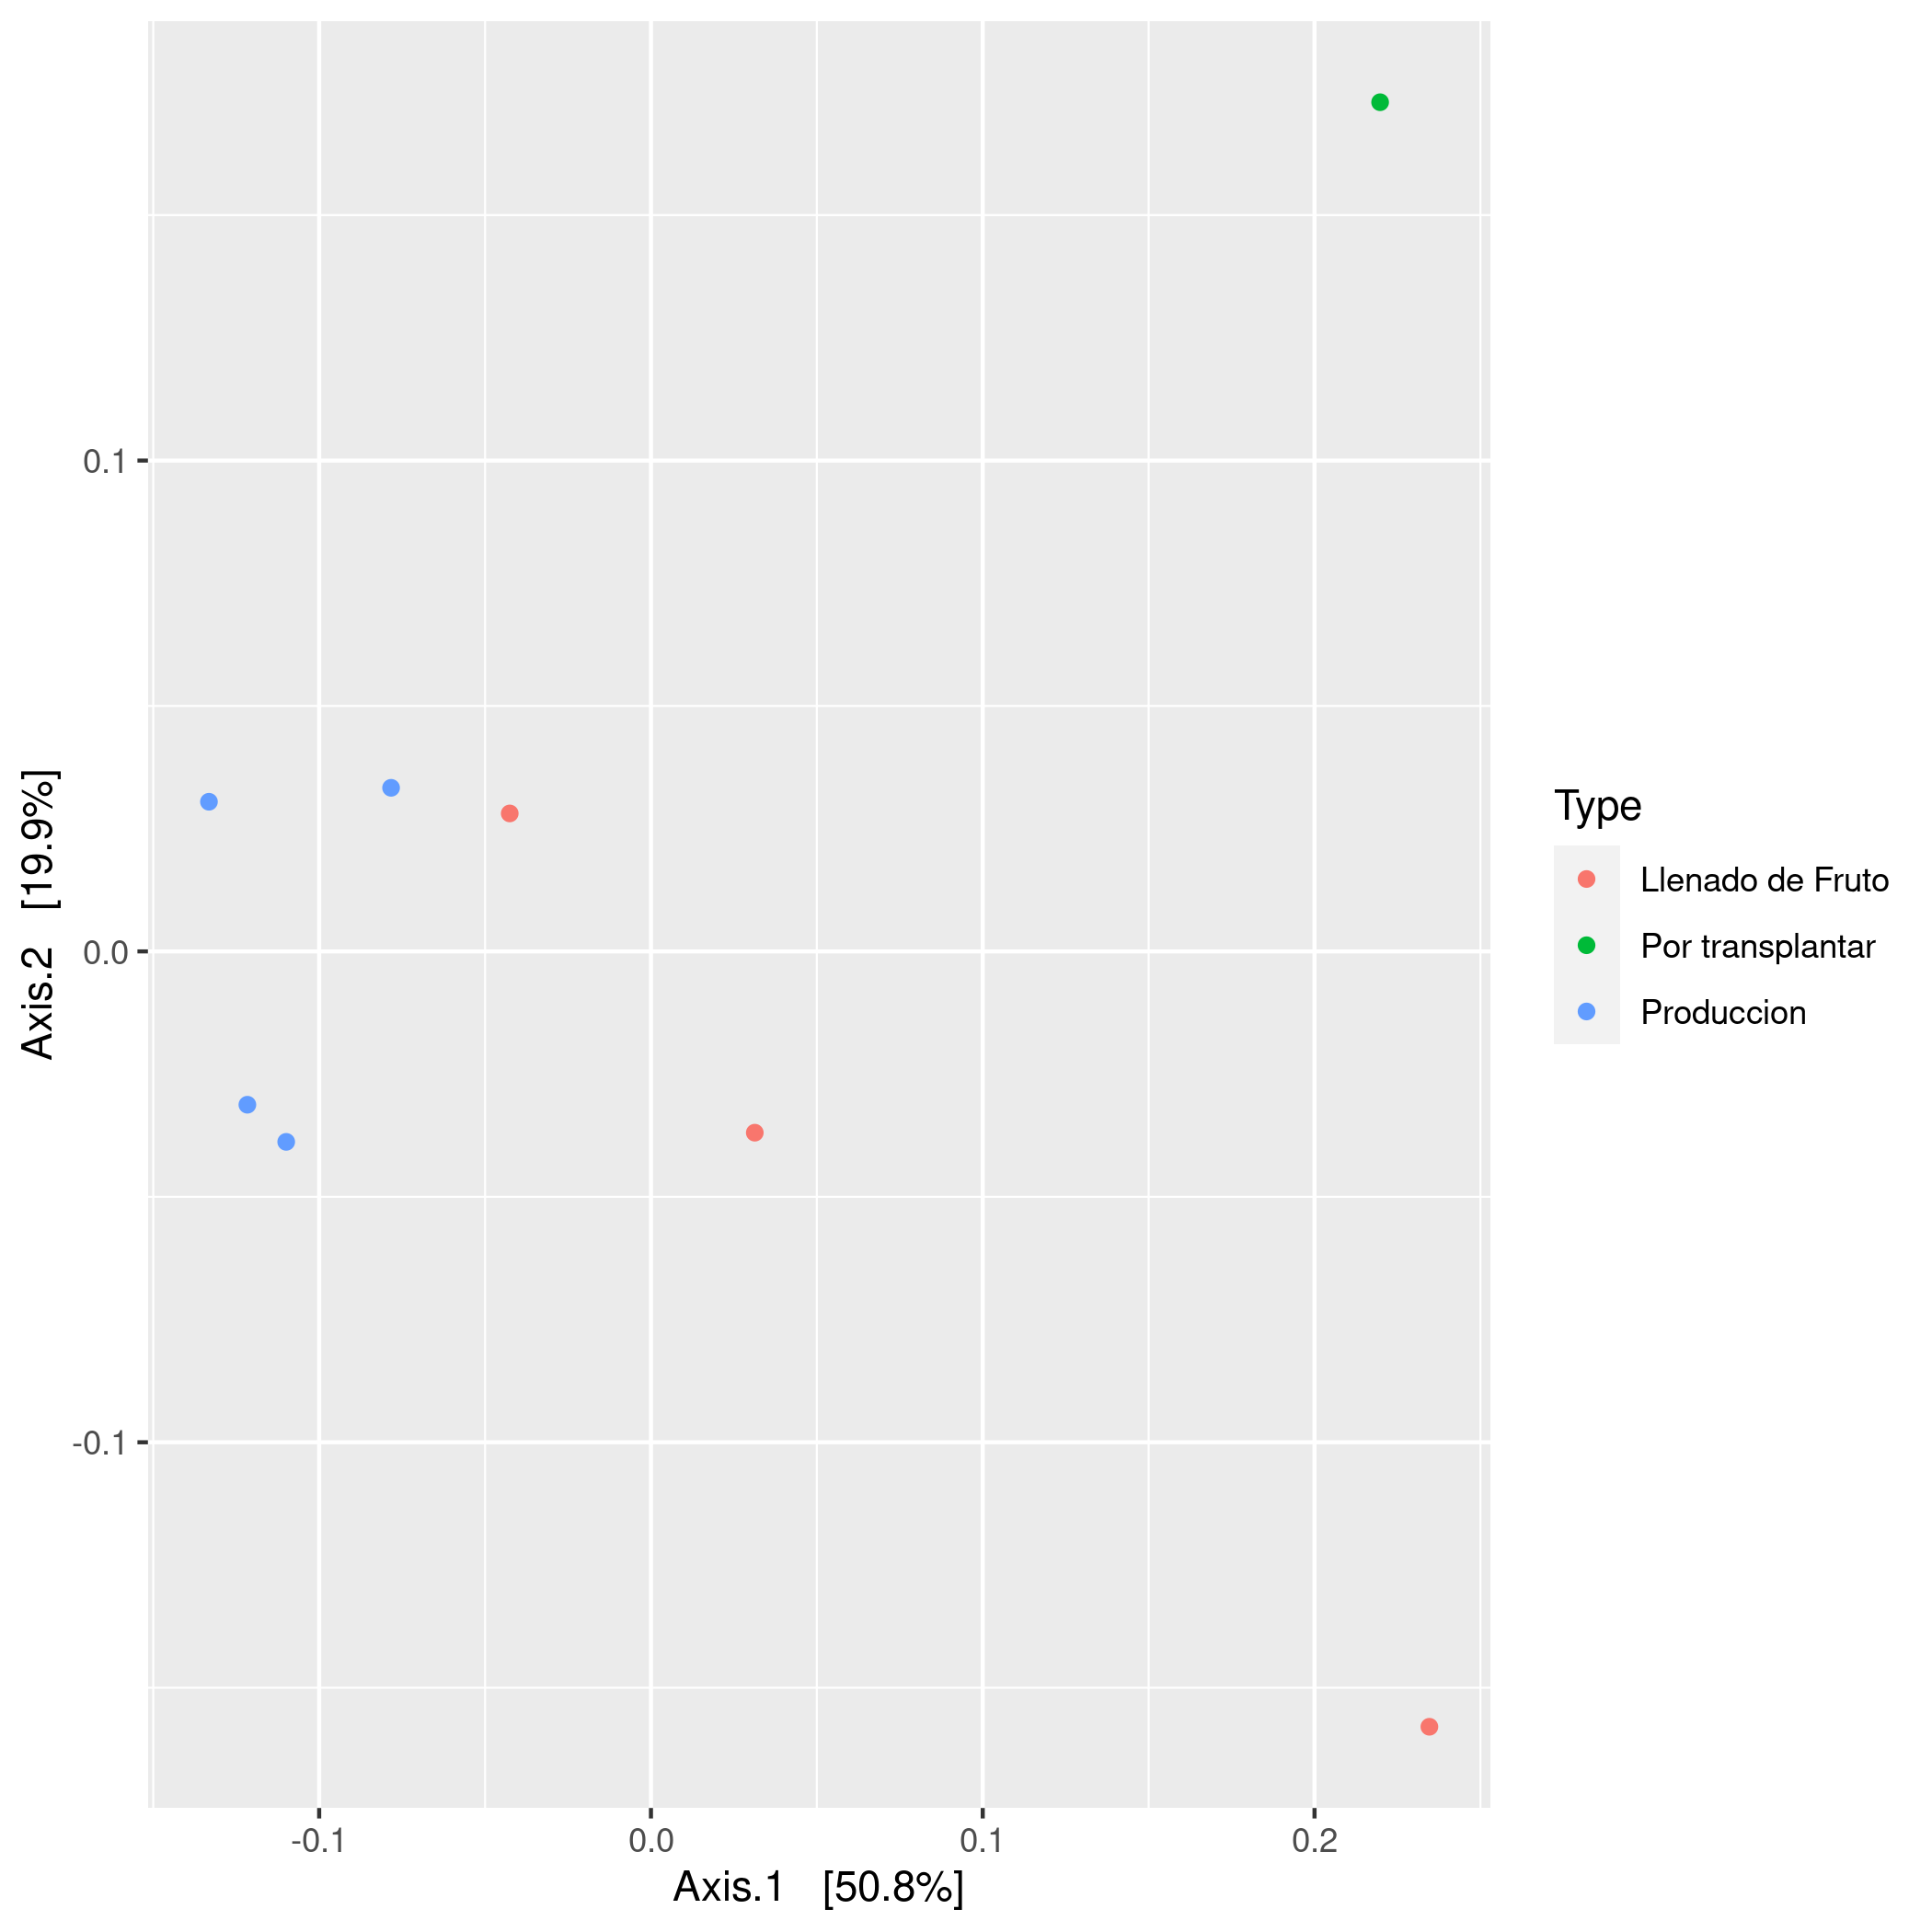
\includegraphics[scale = 0.7]{pcoa_muestras_tomate_no_desarrollo.csv.png}
 \caption{PCoA analysis with Bray-Curtis distance of rhizosphere samples of tomate no desarrollo.csv.}
 \label{fig:tomate_no_desarrollo.csv_pcoa}
\end{figure}
\begin{figure}
  \centering
  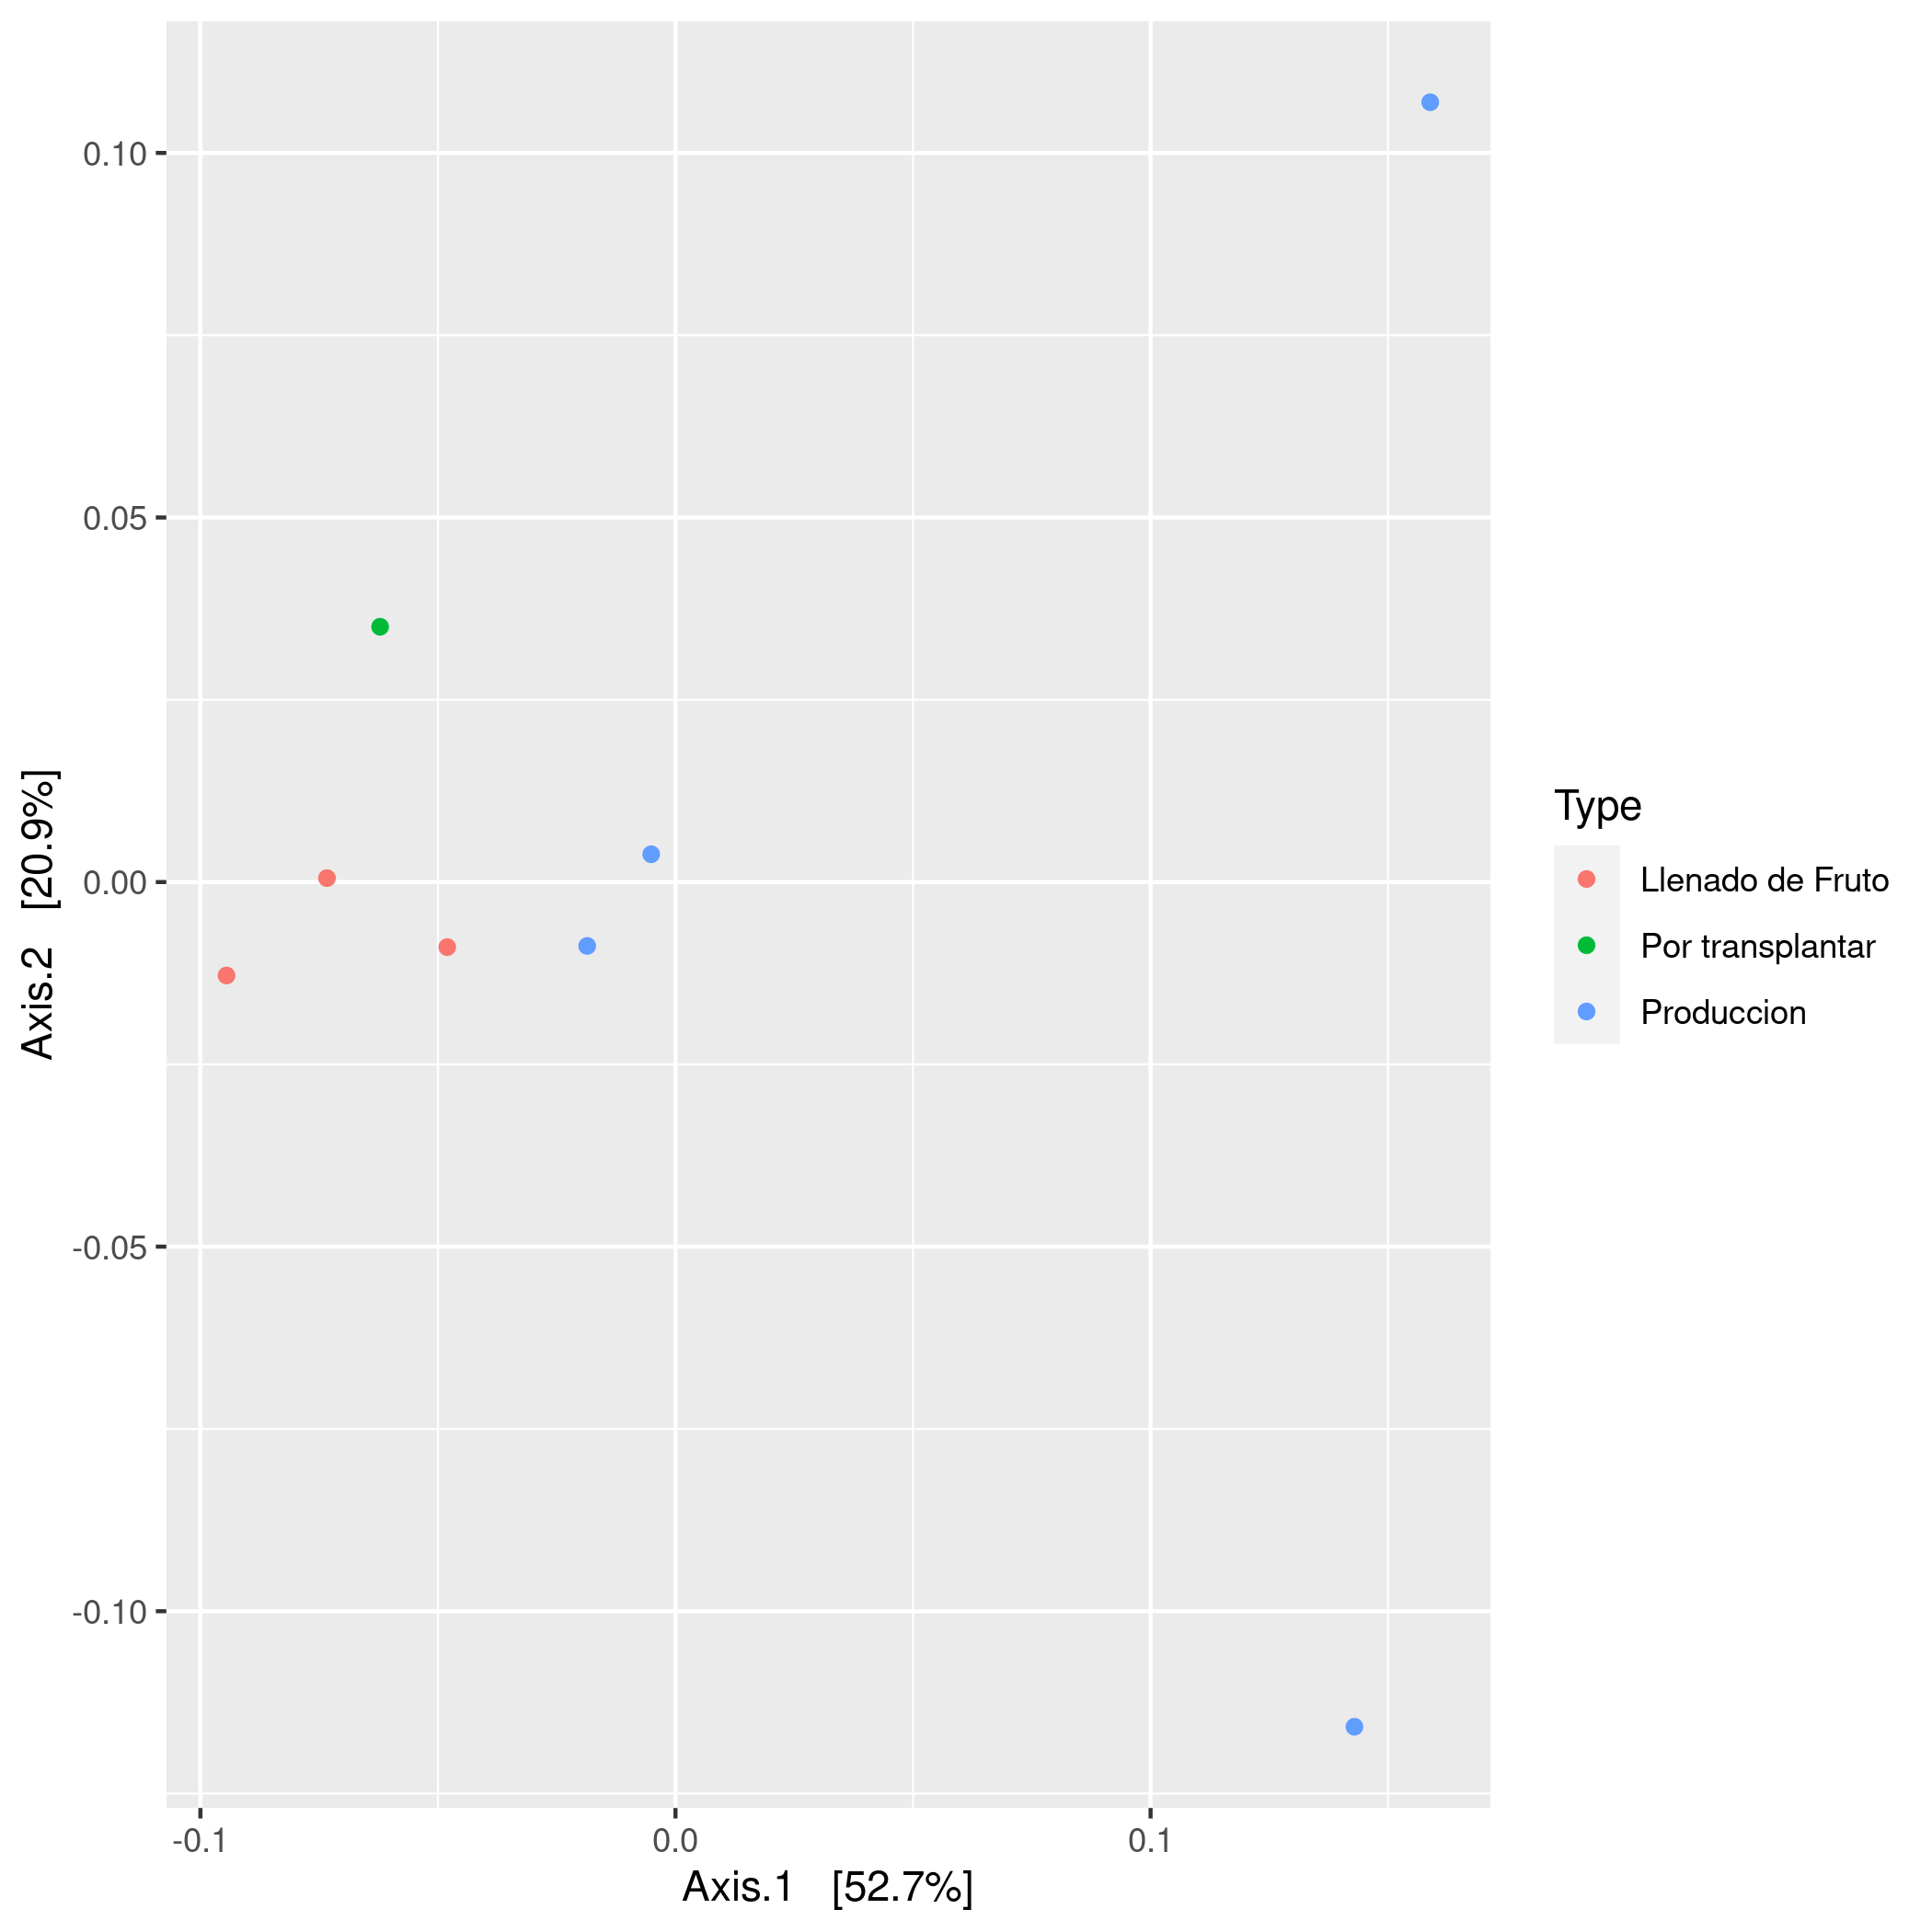
\includegraphics[scale = 0.7]{pcoa_key_otus_tomate_no_desarrollo.csv.png}
  \caption{PCoA analysis with Bray-Curtis distance of rhizosphere samples of tomate no desarrollo.csv, restricted to keystone OTUs.}
  \label{fig:tomate_no_desarrollo.csv_pcoa_key_otus}
\end{figure}



%Candidates to keystone OTUs of rhizosphere of \textit{Solanum lycopersicum} were chosen with the criteria of degree bigger than 51, closeness bigger than 5.6398e-05  and betweenness lower than 1461.0362. 
%From 18 samples of more than 8000 OTUs 37 keystone OTUs were found. 
%This is the highest number of keystone OTUs frome the three analyses present in this report. 

%As seen in Figure \ref{fig:tomate_key_abundance_phyla} phylum \textit{Pseudomonadota} is well represented among keystone OTUs of rhizosphere of \textit{Solanum lycopersicum}, followed by \textit{Actinomycetota}. 
%An important family of \textit{Pseudomonadota} in keystone OTUs is \textit{Burkholderiaceae} (see Figure \ref{tomate_key_abundance_families}).





%Both in number species and in relative abundance \textit{Burkholderia} is a well represented genus among in this report, as well as \textit{Paraburkholderia}, some of whose species are known to improve tomato seedling growth (see \cite{Caradonia2022}). 
%.Genus \textit{Pseudomonas}, several of whose species have been observed to inhibit the bacterial wilt in tomato (see \cite{Mohammed2020}), was also present among keystone OTUs.
%Both \textit{Pseudarthrobacter} and \textit{Candidatus Nitrosocosmicus}, found as keystone OTUs in this study, have been found as \textit{hub taxa} of the rhizosphere of other plants (see \cite{Floch2020}).


%As seen in Figure \ref{mean_median_tomate} all candidate to keystone OTUs are well represented through all samples, being in median and mean of relative abundance above the mean relative abundance of all OTUs.



%Most of the samples, but one of them, become more similar when restricting to keystone OTUs, according to a PCoA analyses with Bray-Curtis distance (see Figures \ref{fig:tomate_pcoa} and \ref{fig:tomate_pcoa_key_otus}). 






\begin{figure}
    \centering
    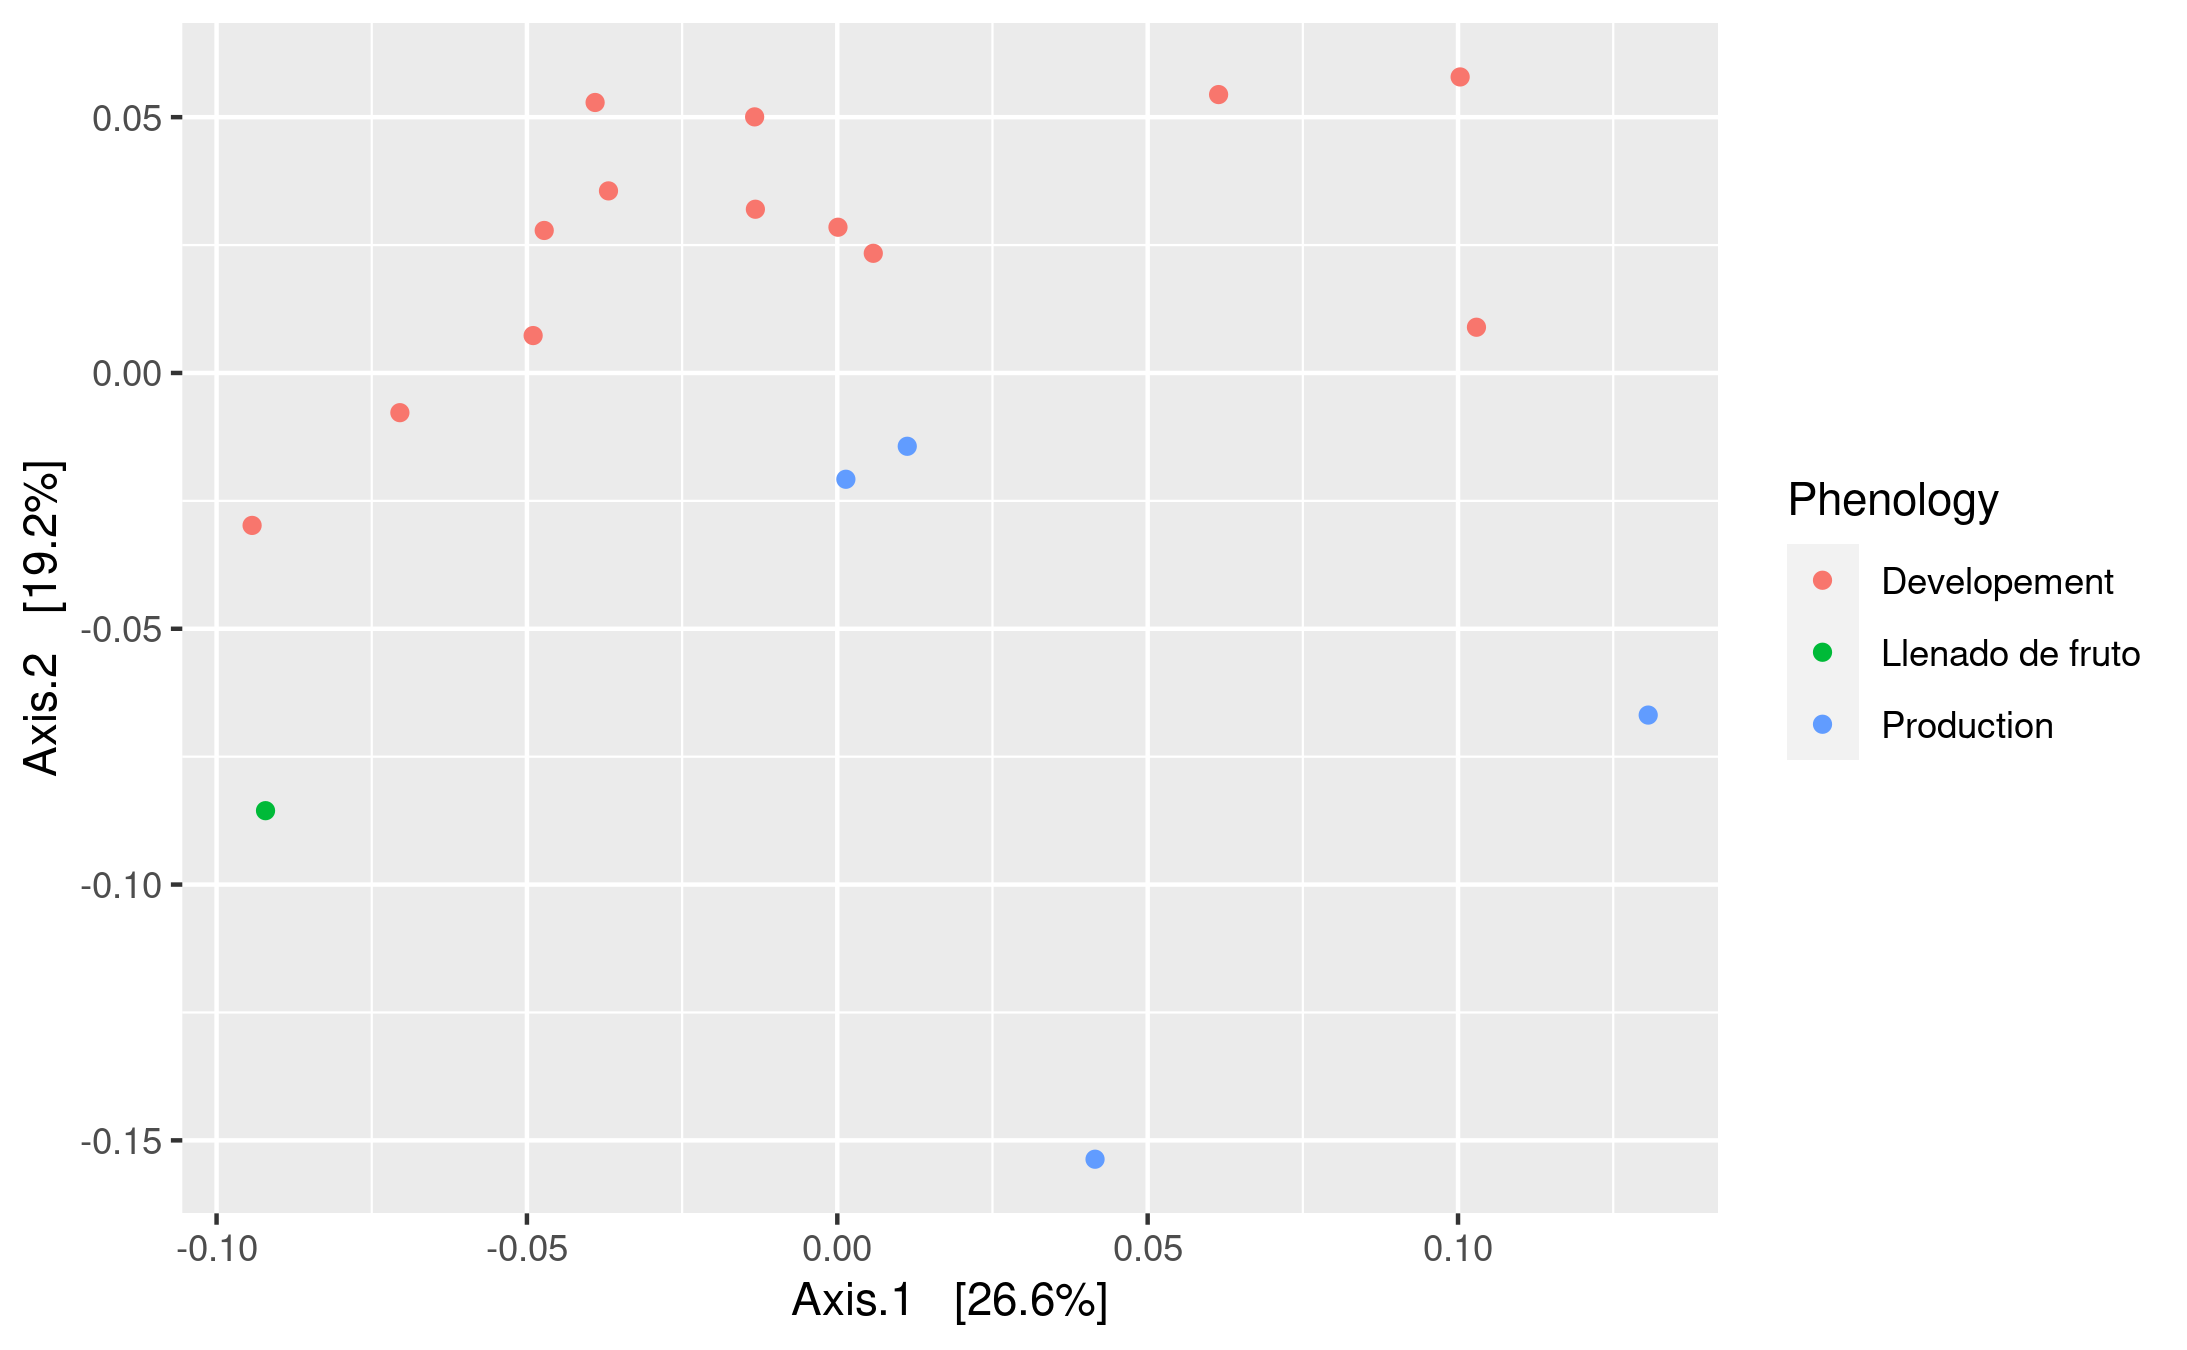
\includegraphics[scale = 0.7]{tomate_muestras_pcoa.png}
    \caption{PCoA analysis with Bray-Curtis distance of rhizosphere samples of \textit{Solanum lycopersicum}.}
    \label{fig:tomate_pcoa}
\end{figure}

\begin{figure}
    \centering
    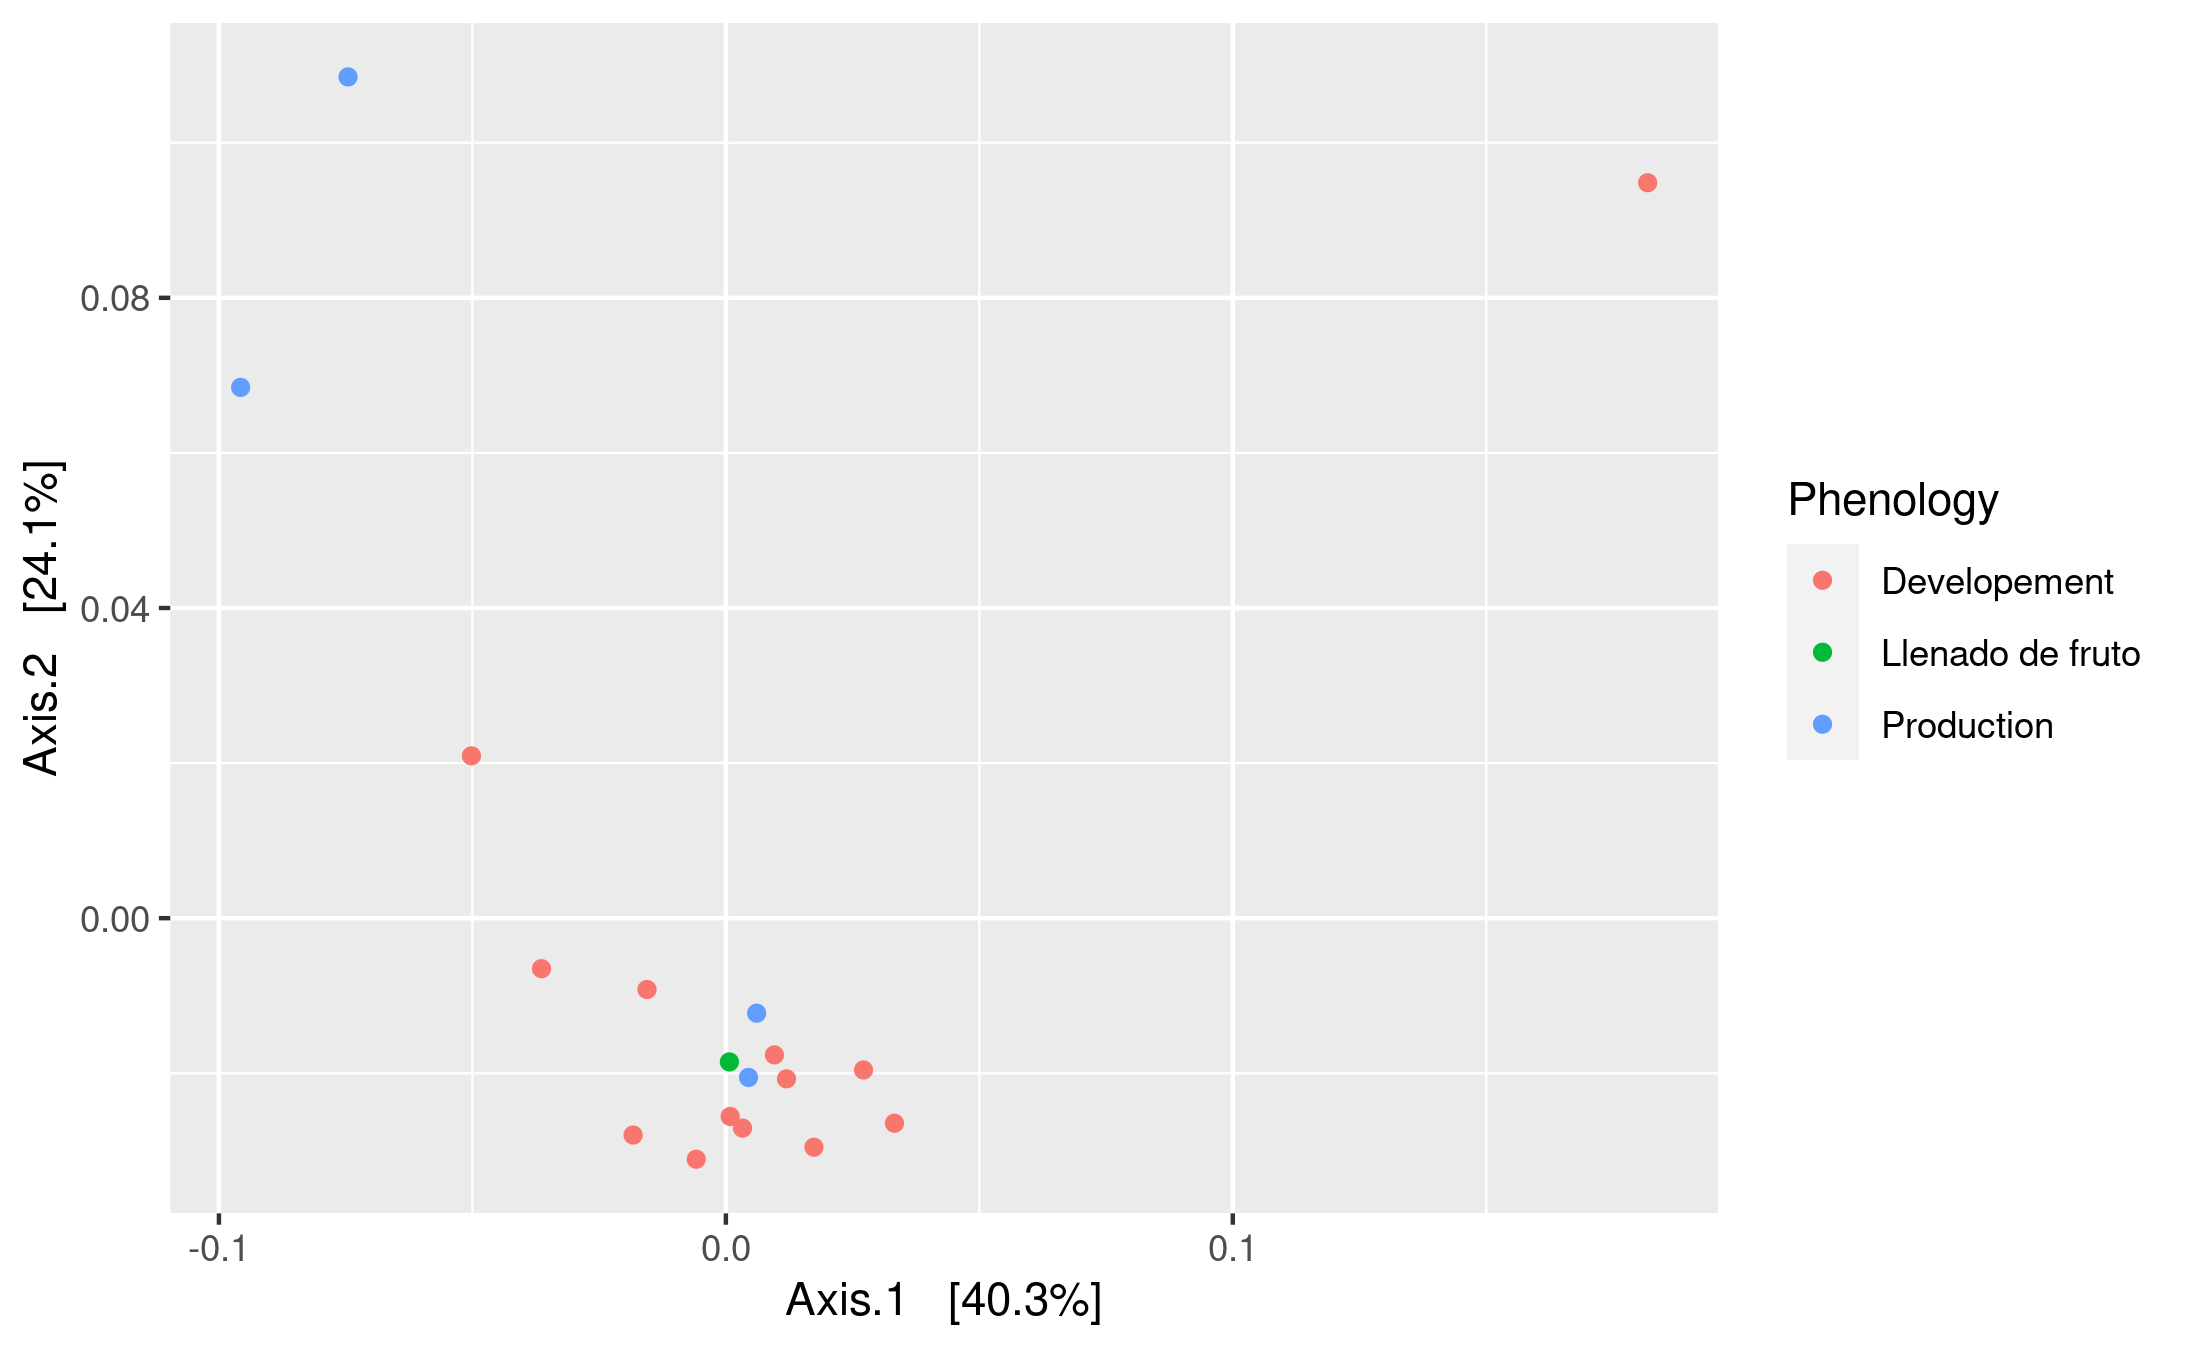
\includegraphics[scale = 0.7]{tomate_clave_pcoa.png}
    \caption{PCoA analysis with Bray-Curtis distance of rhizosphere samples of \textit{Solanum lycopersicum}, restricted to keystone OTUs.}
    \label{fig:tomate_pcoa_key_otus}
\end{figure}


\section{10 random subsamples}

\begin{figure}
\centering
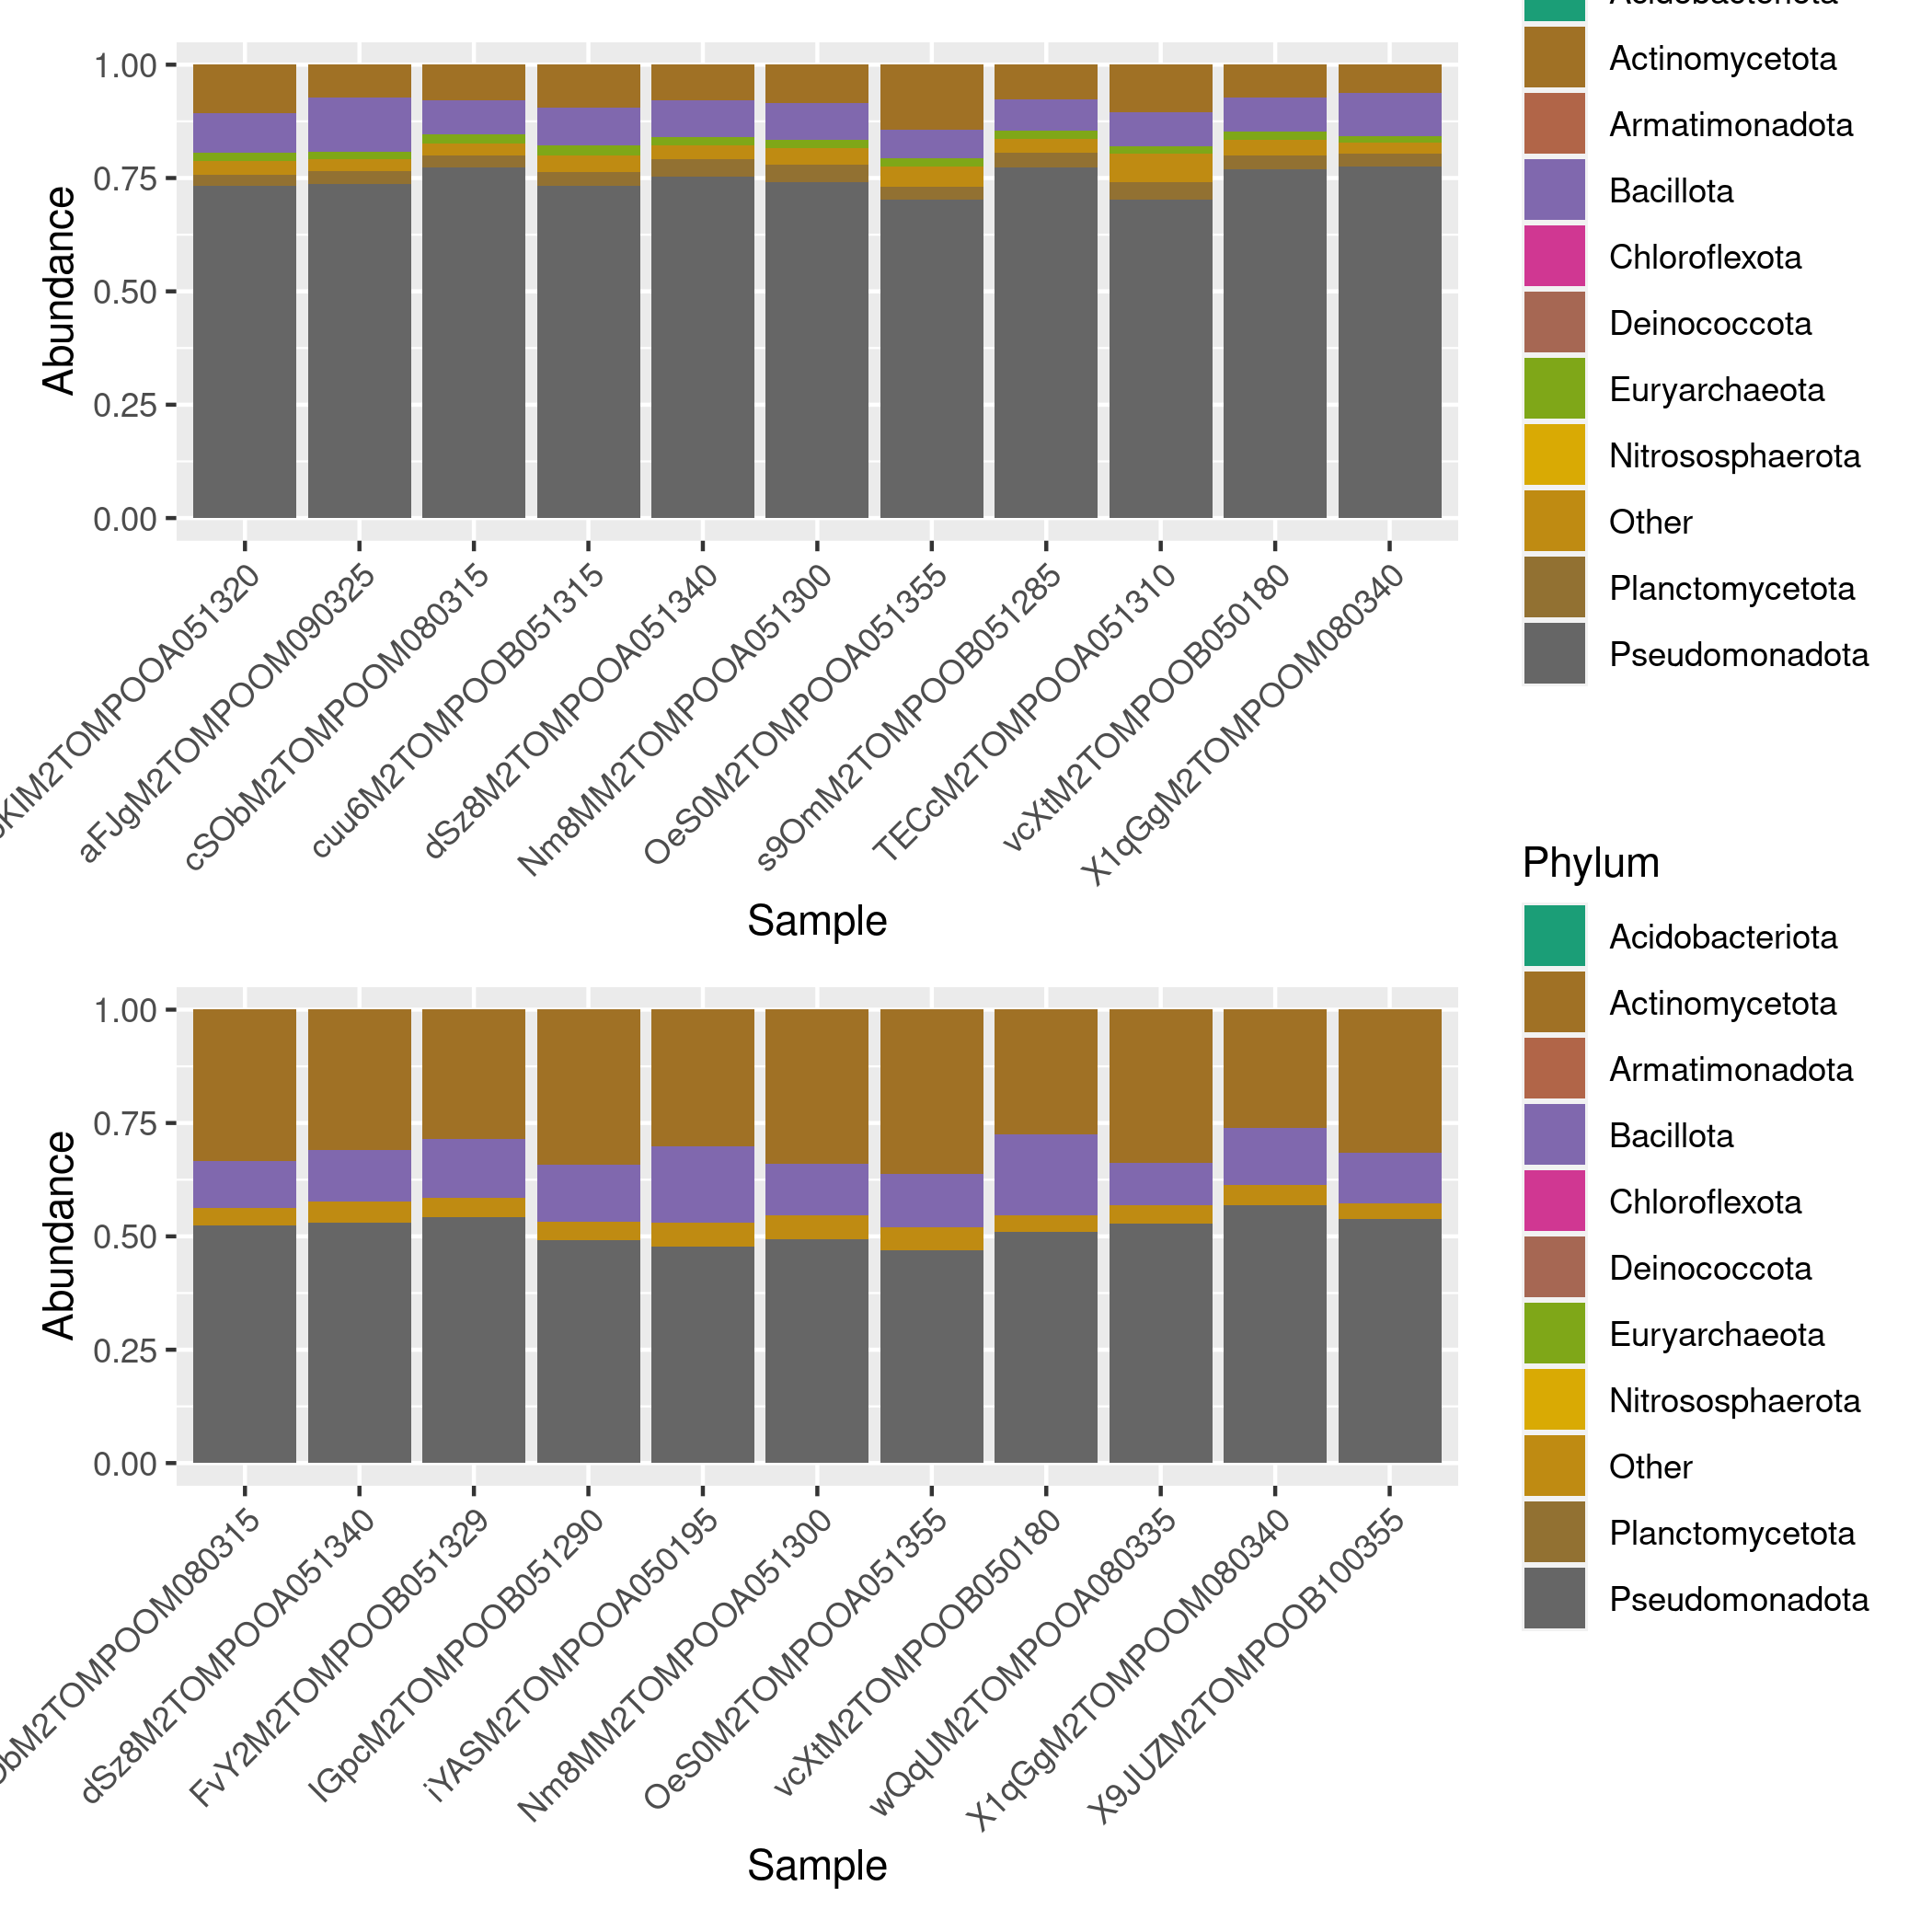
\includegraphics[scale=0.8]{otus_centrales_tomate_aleatorio1_1.csv_otus_centrales_tomate_aleatorio1_2.csv_relative_abundance_Phylum.png}
\caption{Comparison of reports from random subsamples 1 and 2 by Phylum}
\end{figure}


\begin{figure}
\centering
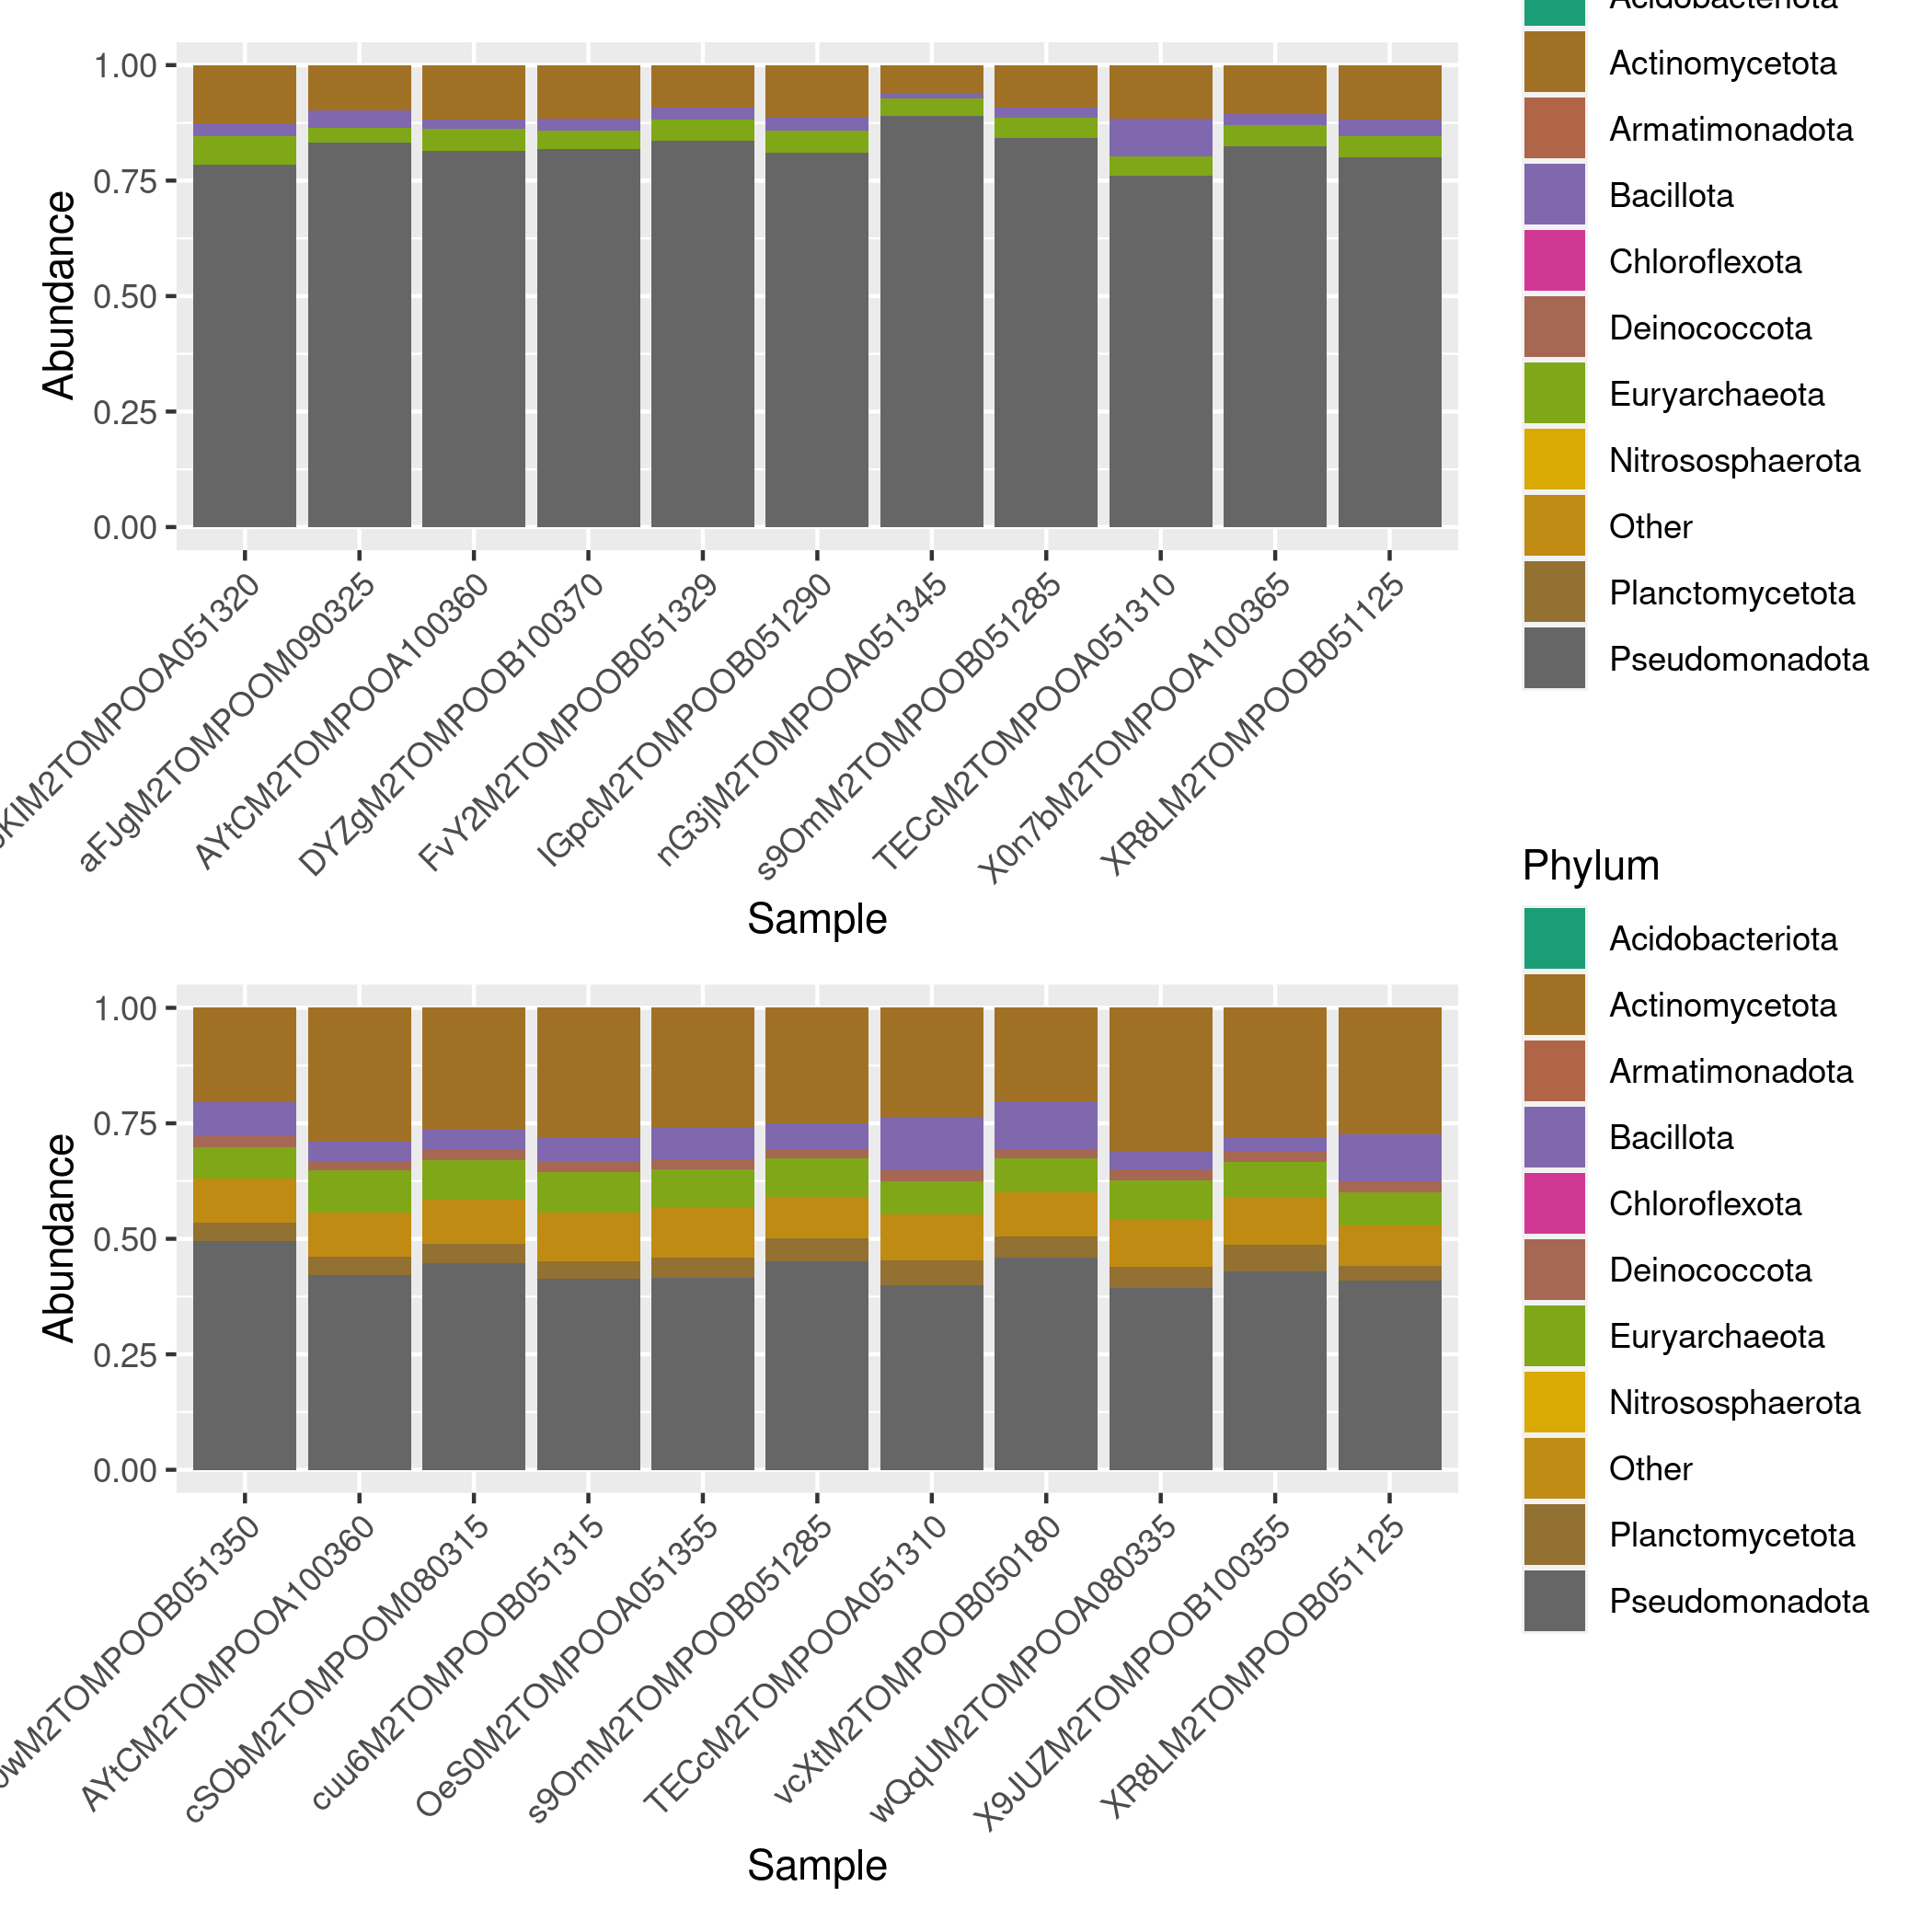
\includegraphics[scale=0.8]{otus_centrales_tomate_aleatorio1_3.csv_otus_centrales_tomate_aleatorio1_4.csv_relative_abundance_Phylum.png}
\caption{Comparison of reports from random subsamples 3 and 4 by Phylum}
\end{figure}


\begin{figure}
\centering
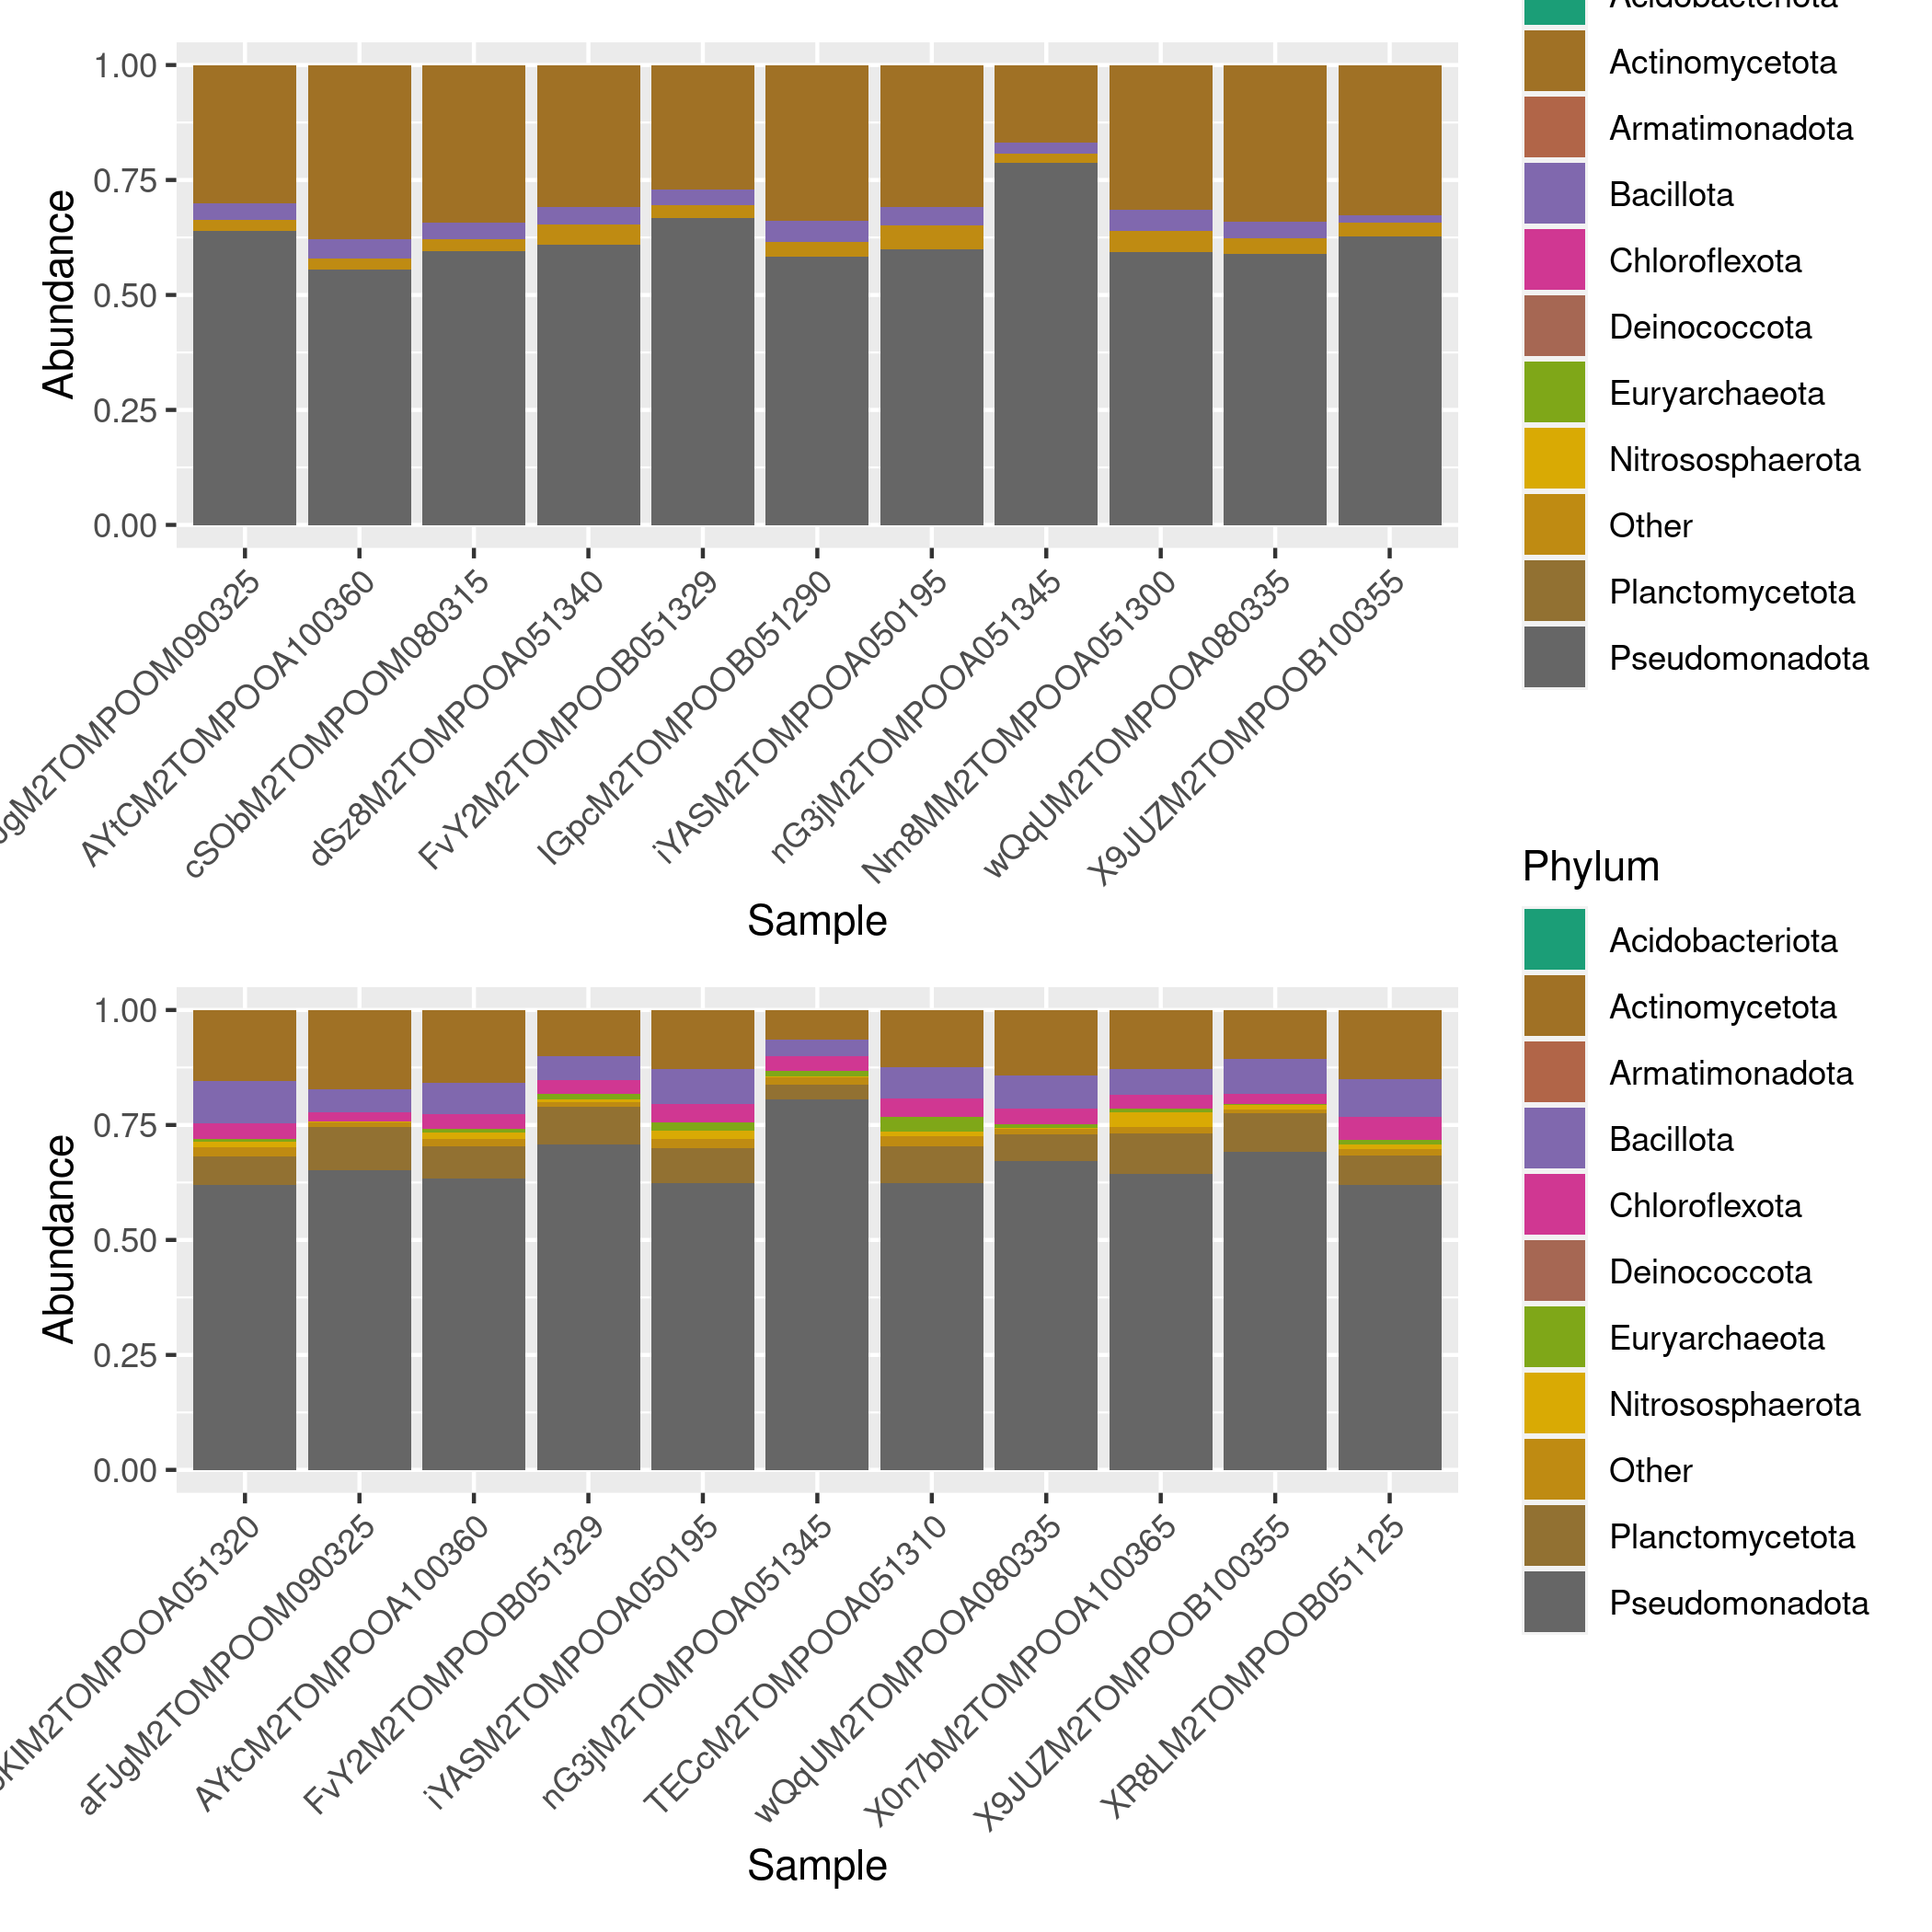
\includegraphics[scale=0.8]{otus_centrales_tomate_aleatorio1_5.csv_otus_centrales_tomate_aleatorio1_6.csv_relative_abundance_Phylum.png}
\caption{Comparison of reports from random subsamples 5 and 6 by Phylum}
\end{figure}


\begin{figure}
\centering
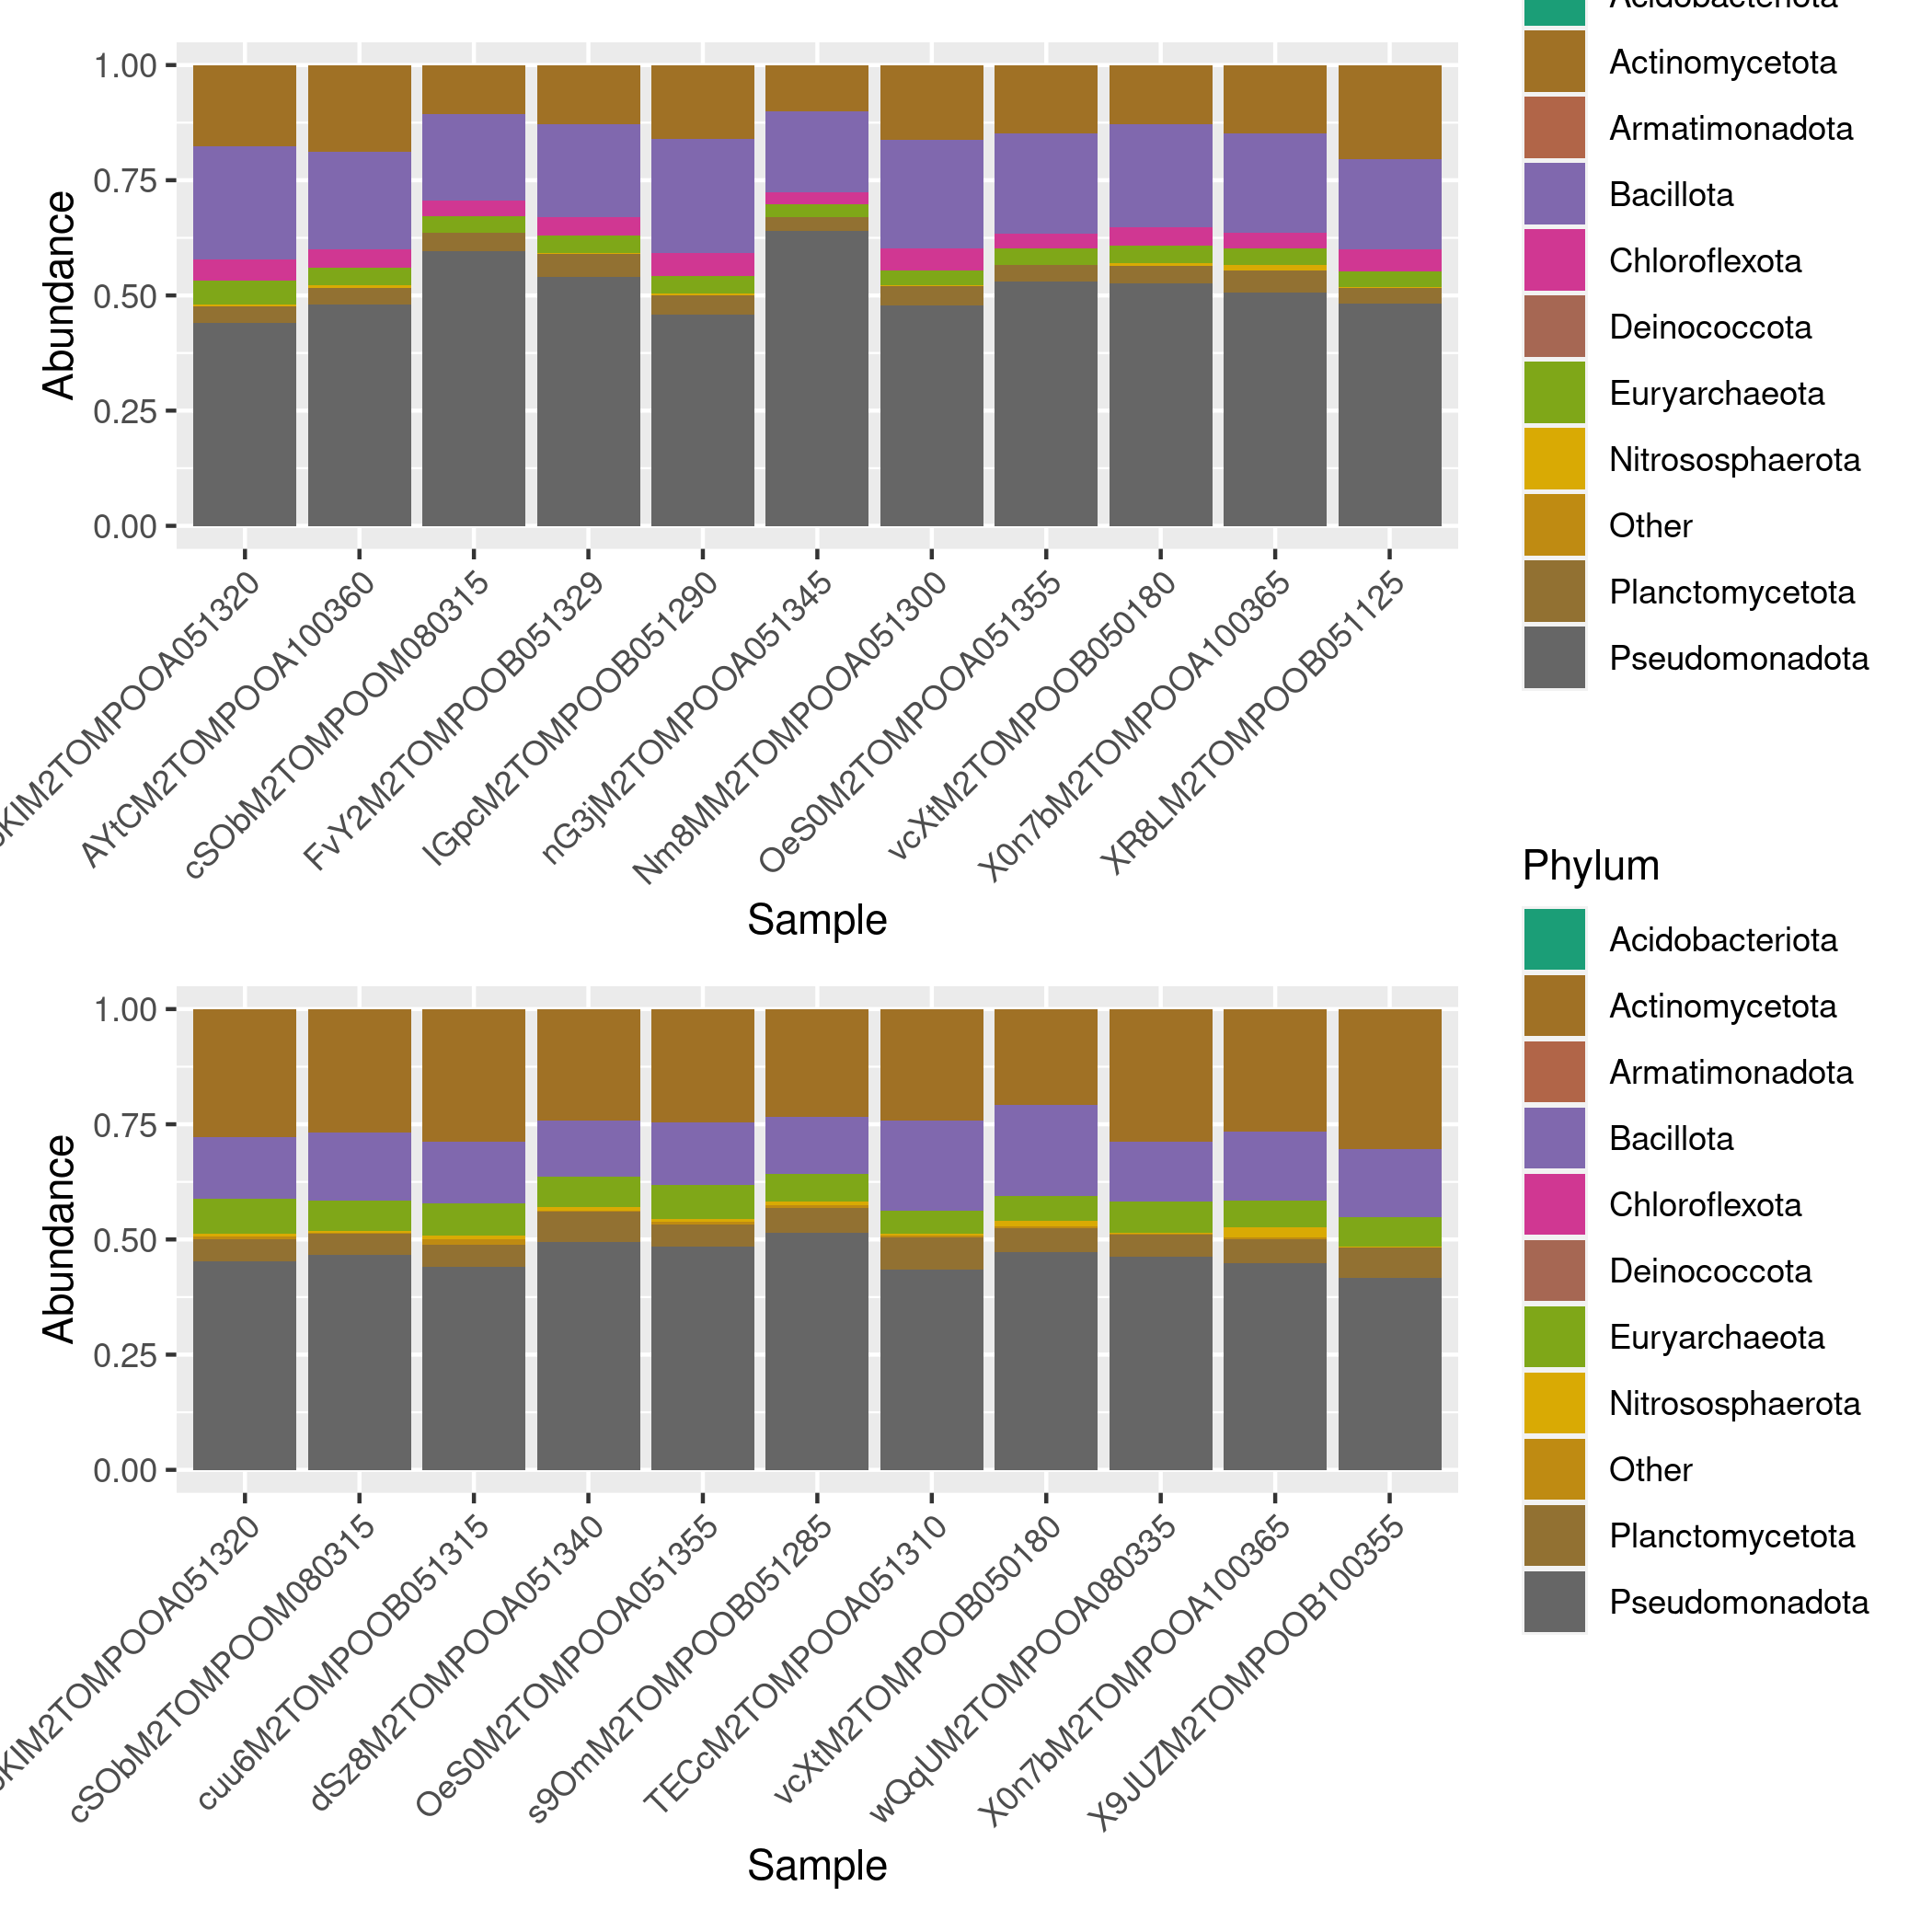
\includegraphics[scale=0.8]{otus_centrales_tomate_aleatorio1_7.csv_otus_centrales_tomate_aleatorio1_8.csv_relative_abundance_Phylum.png}
\caption{Comparison of reports from random subsamples 7 and 8 by Phylum}
\end{figure}


\begin{figure}
\centering
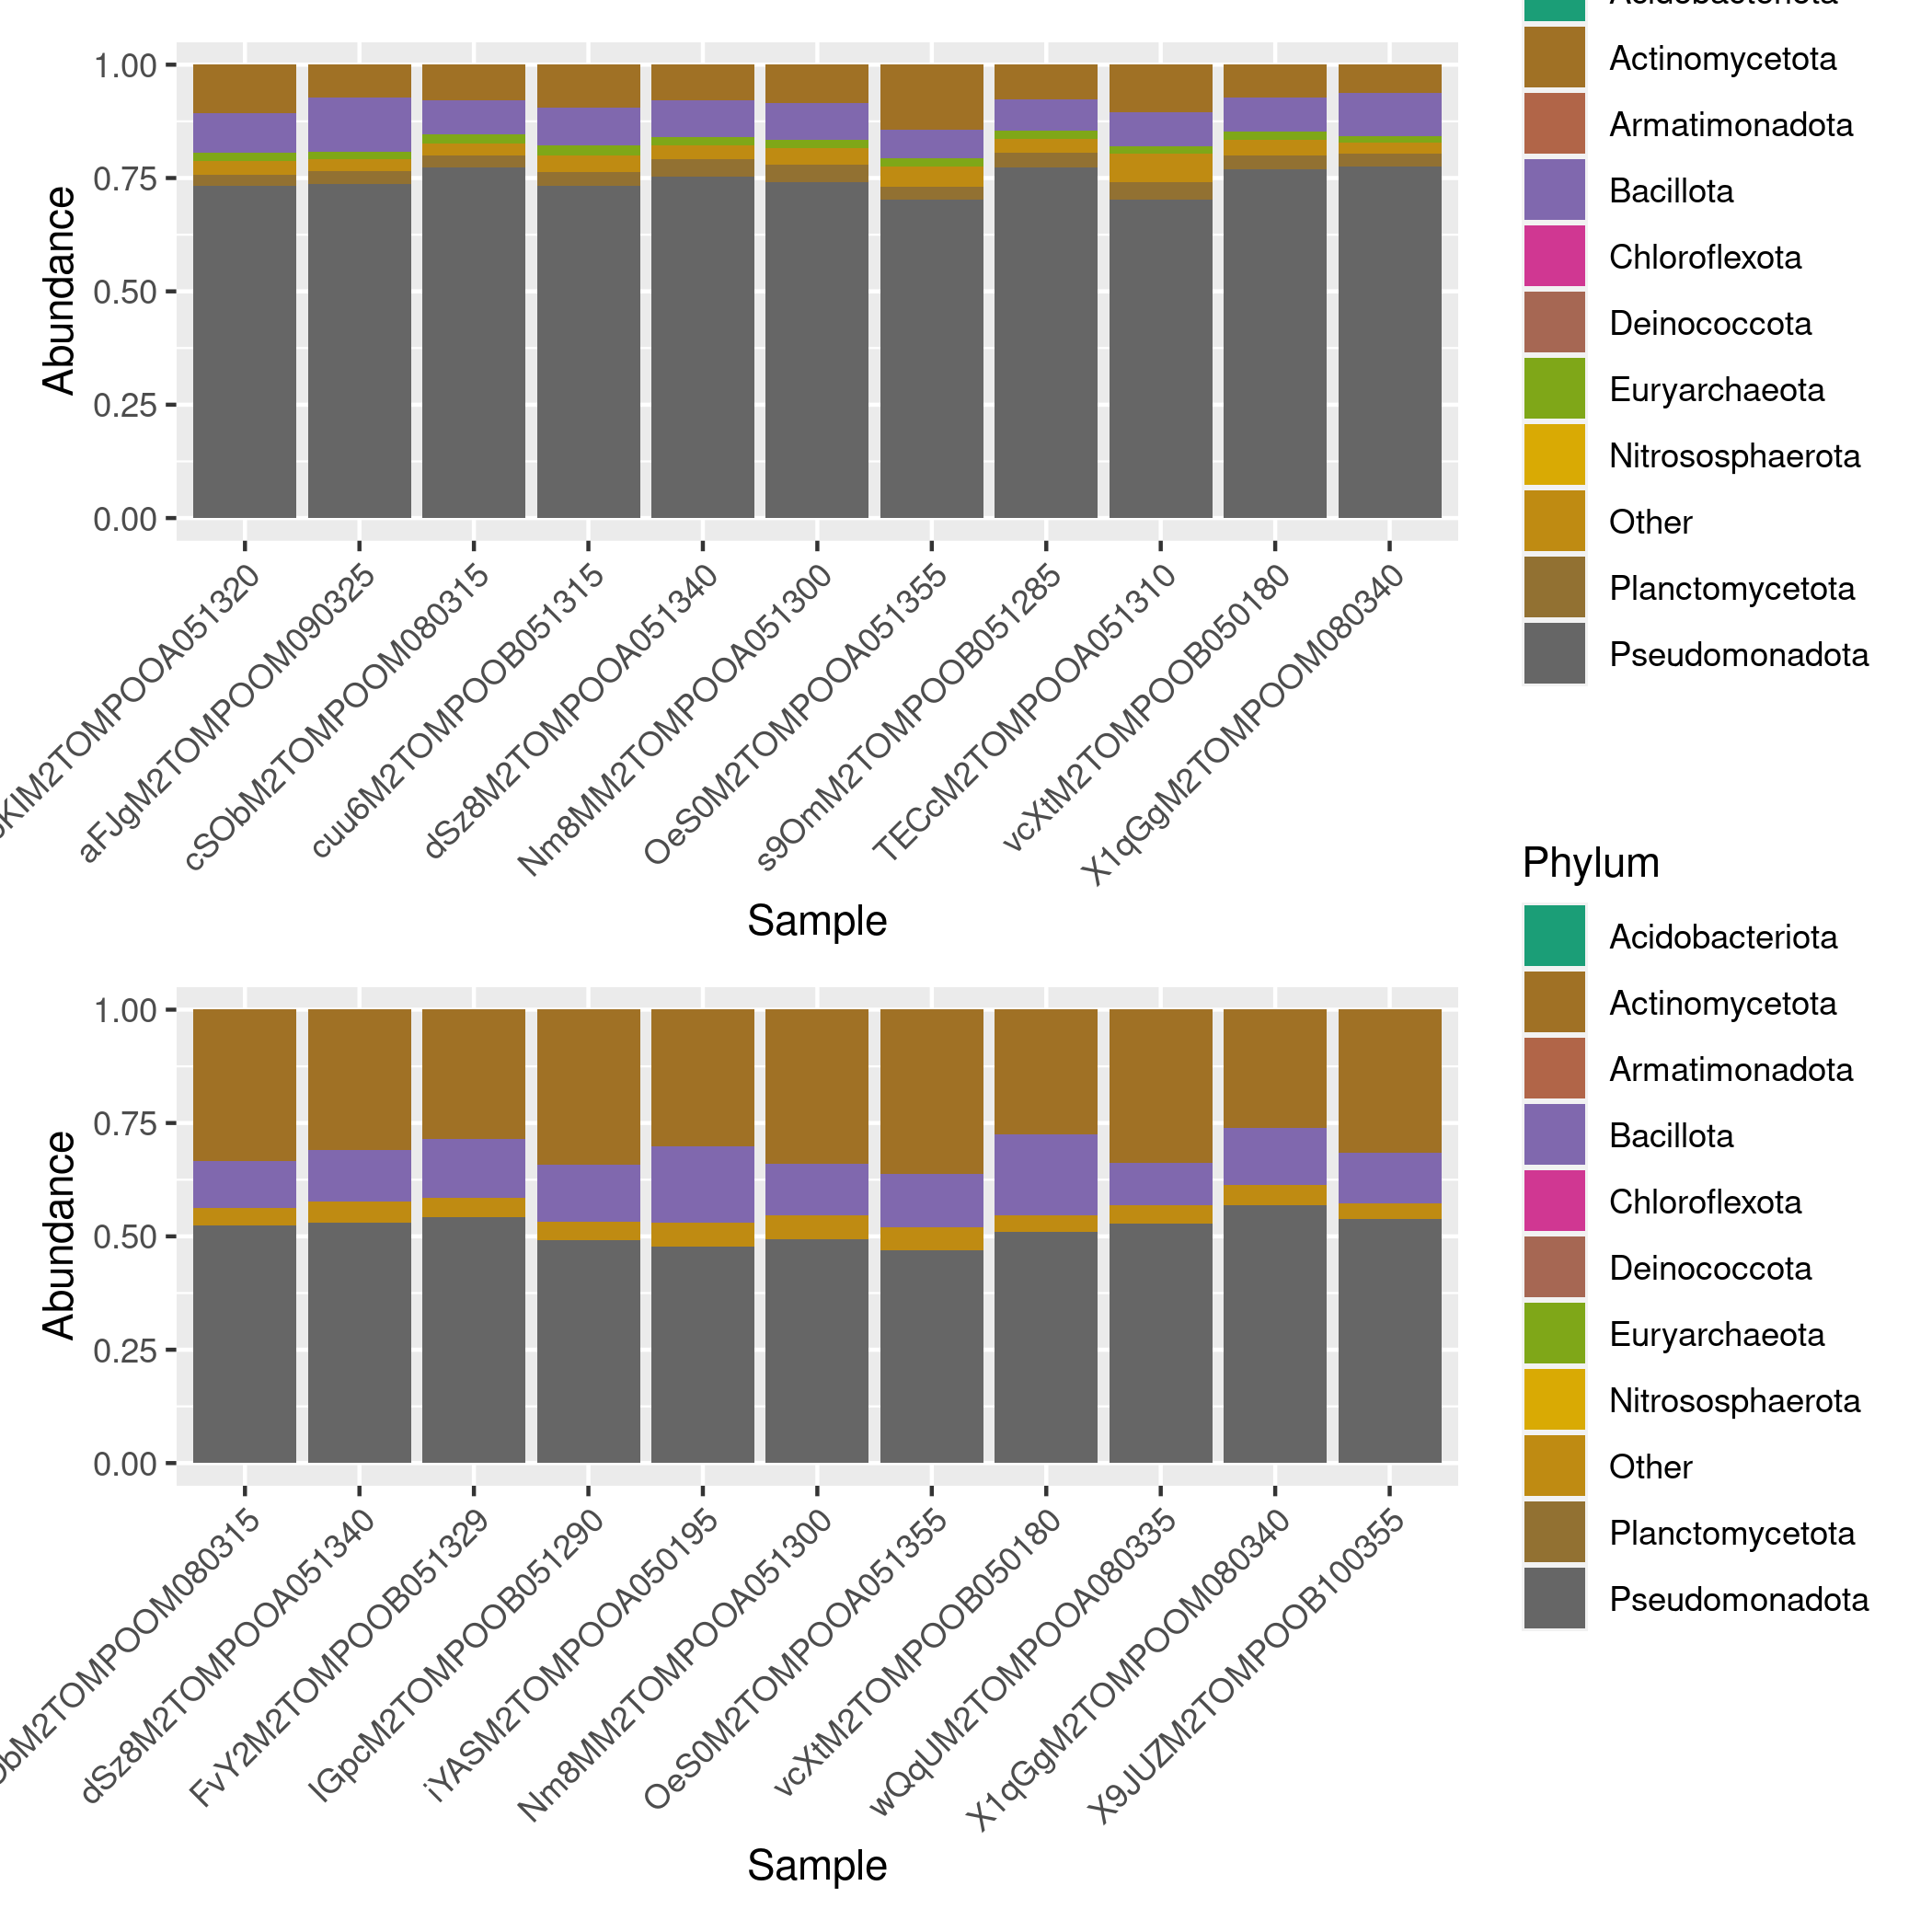
\includegraphics[scale=0.8]{otus_centrales_tomate_aleatorio1_1.csv_otus_centrales_tomate_aleatorio1_2.csv_relative_abundance_Phylum.png}
\caption{Comparison of reports from random subsamples 9 and 10 by Phylum}
\end{figure}

\begin{figure}
\centering
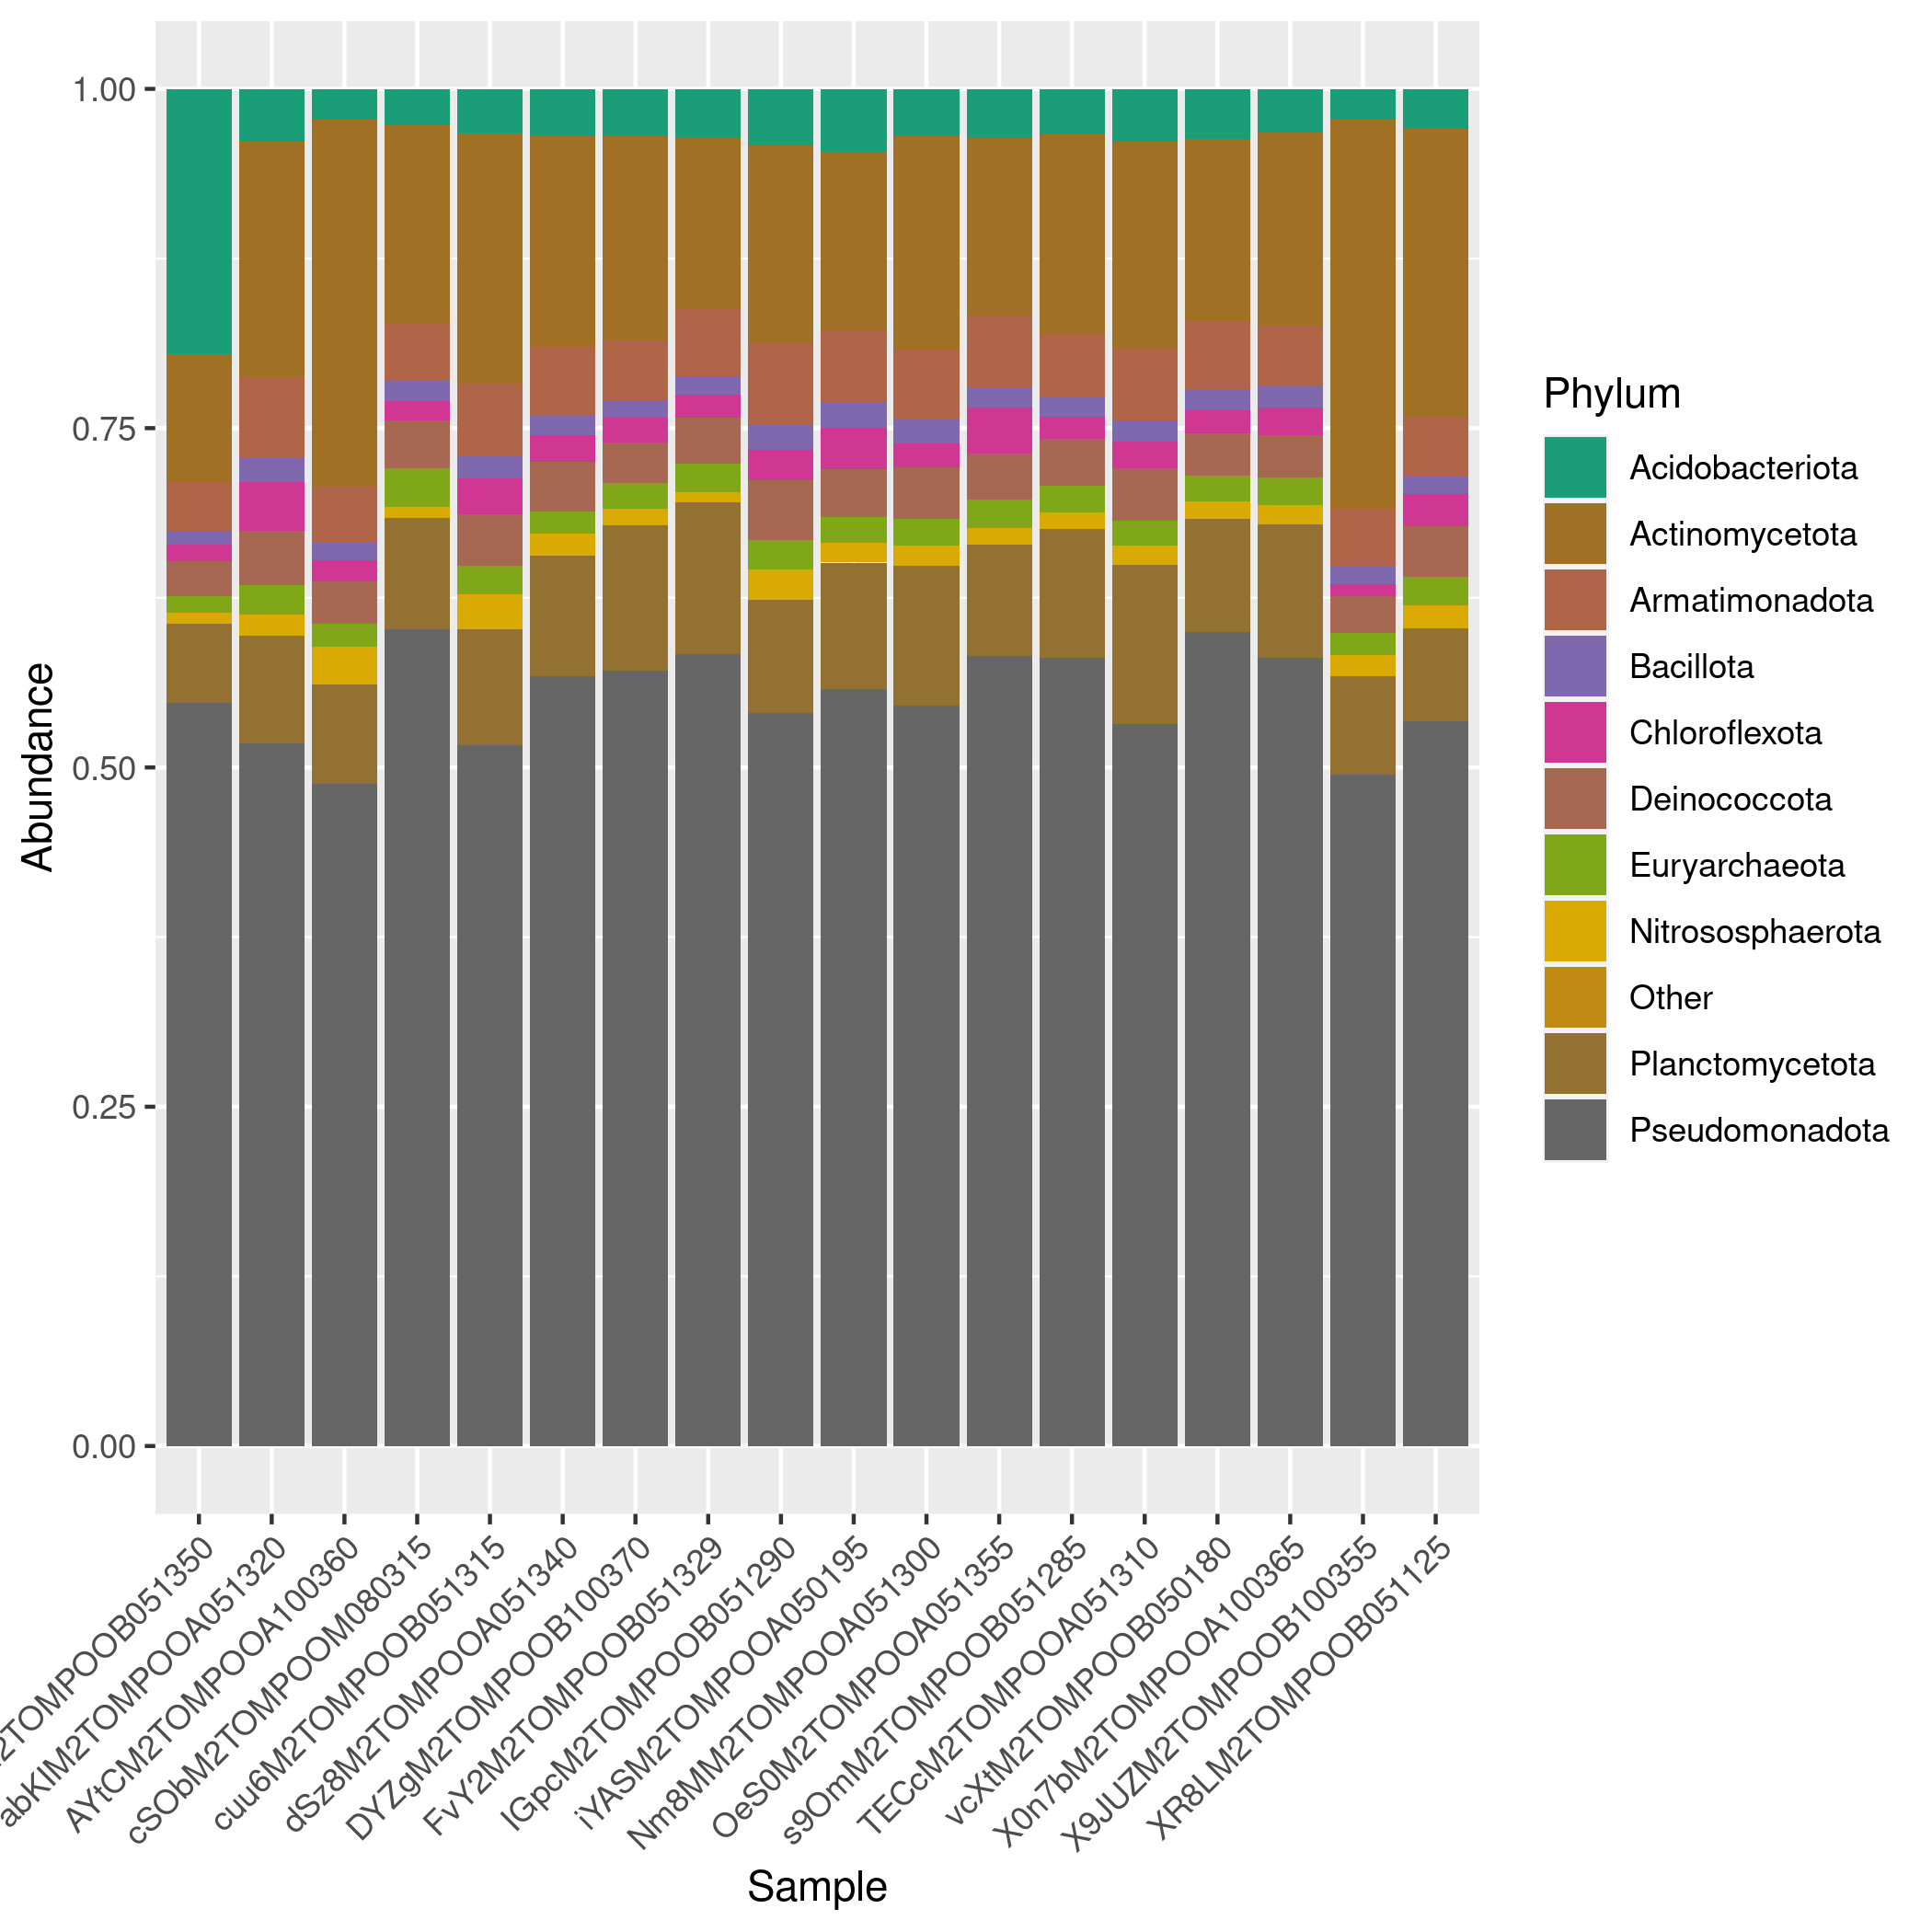
\includegraphics[scale=0.8]{reporte_tomate1.csv_NA_relative_abundance_Phylum.png}
\caption{Comparison of reports from random subsamples 9 and 10 by Phylum}
\end{figure}

\begin{figure}
\centering
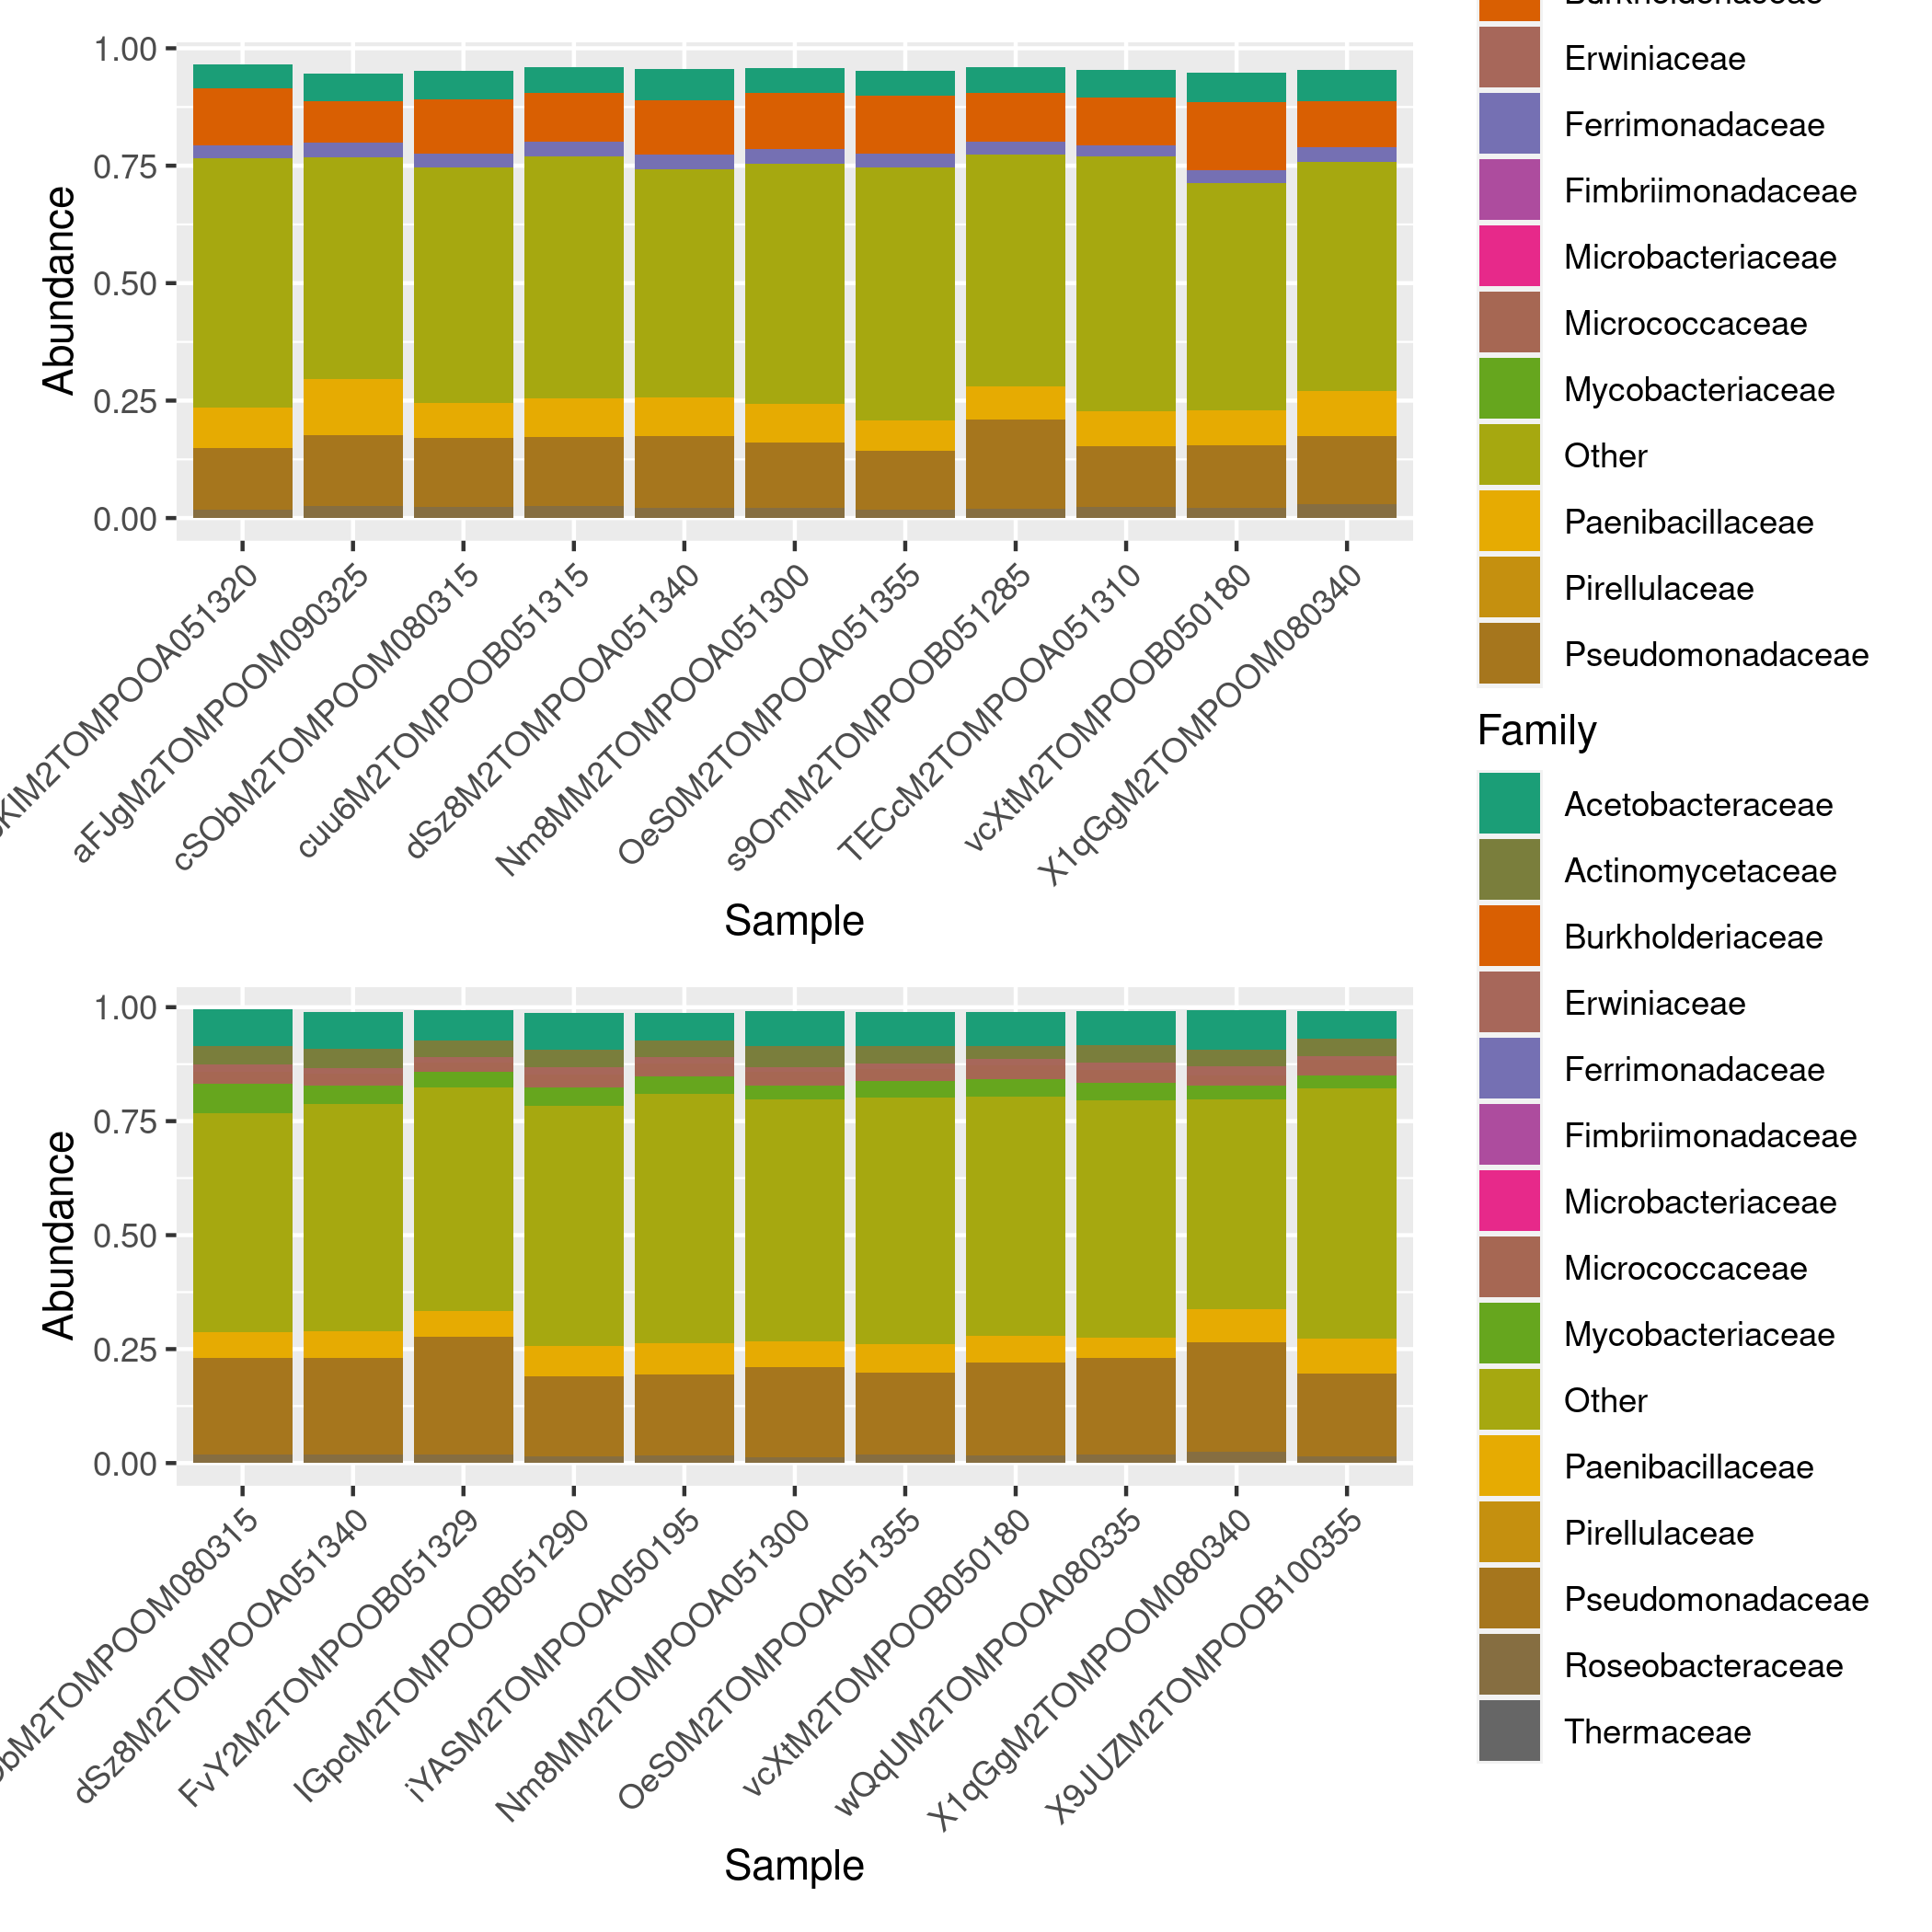
\includegraphics[scale=0.8]{otus_centrales_tomate_aleatorio1_1.csv_otus_centrales_tomate_aleatorio1_2.csv_relative_abundance_Family.png}
\caption{Comparison of reports from random subsamples 1 and 2 by Phylum}
\end{figure}


\begin{figure}
\centering
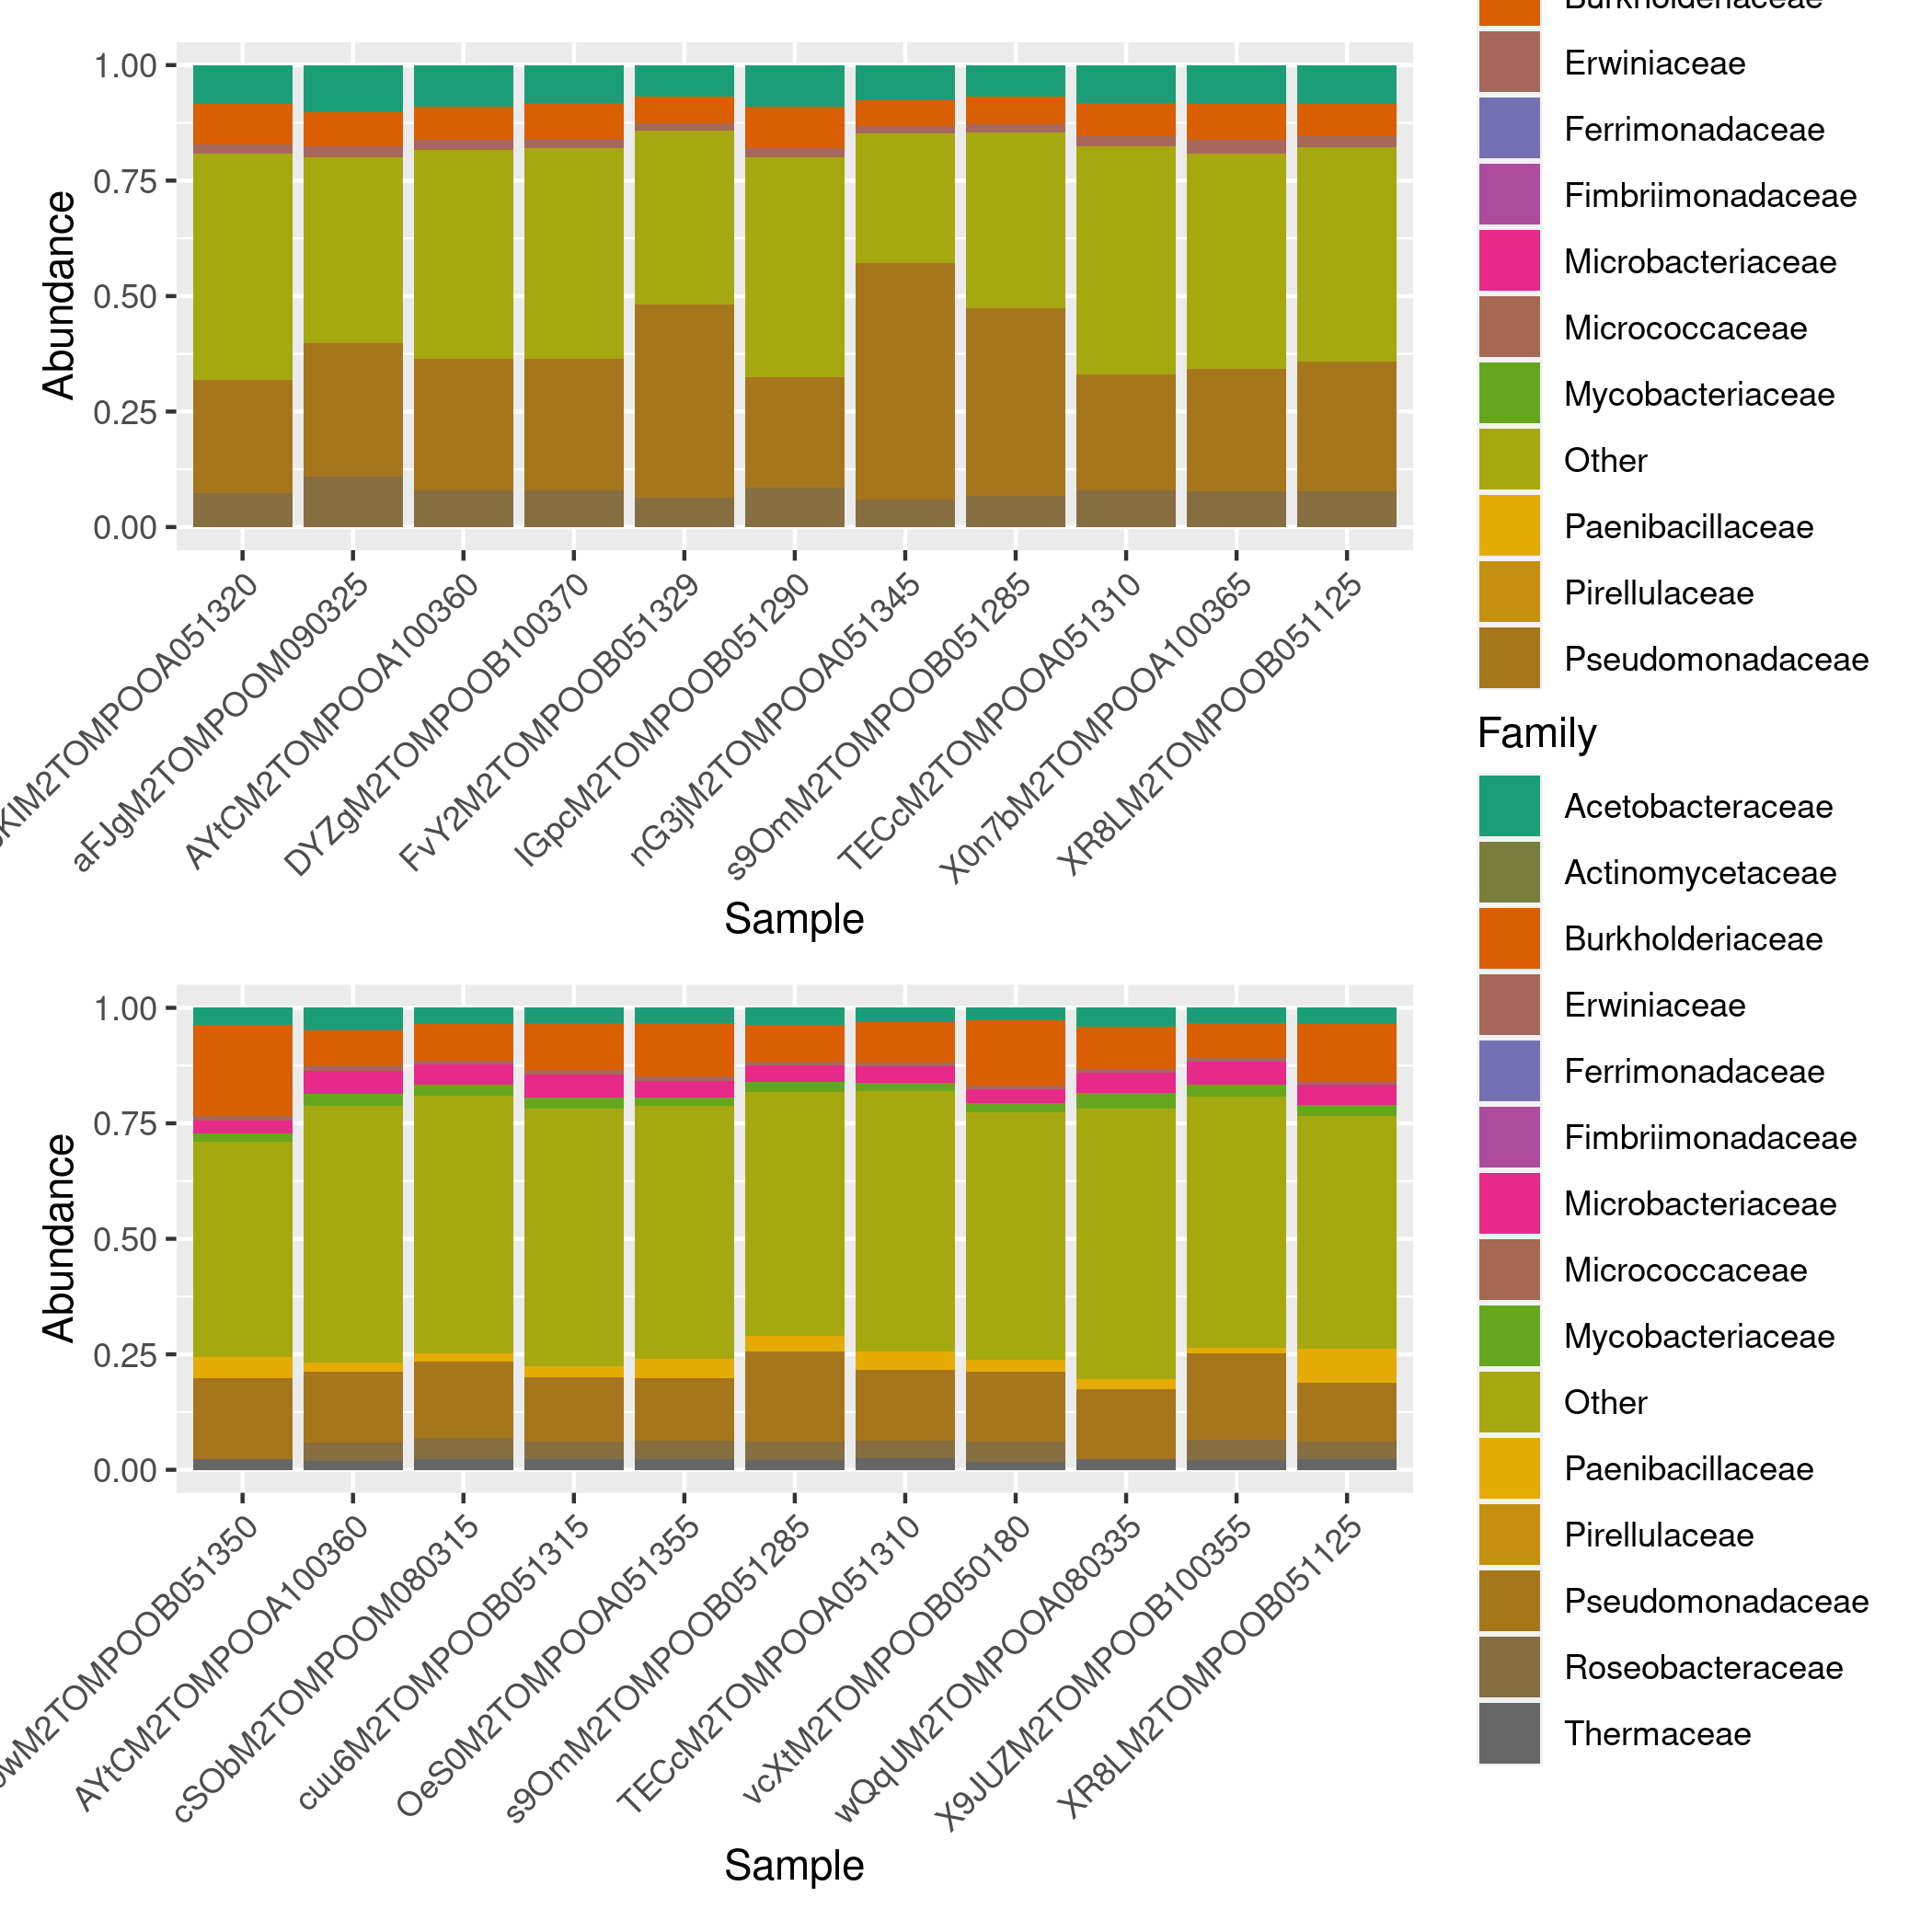
\includegraphics[scale=0.8]{otus_centrales_tomate_aleatorio1_3.csv_otus_centrales_tomate_aleatorio1_4.csv_relative_abundance_Family.png}
\caption{Comparison of reports from random subsamples 3 and 4 by Phylum}
\end{figure}


\begin{figure}
\centering
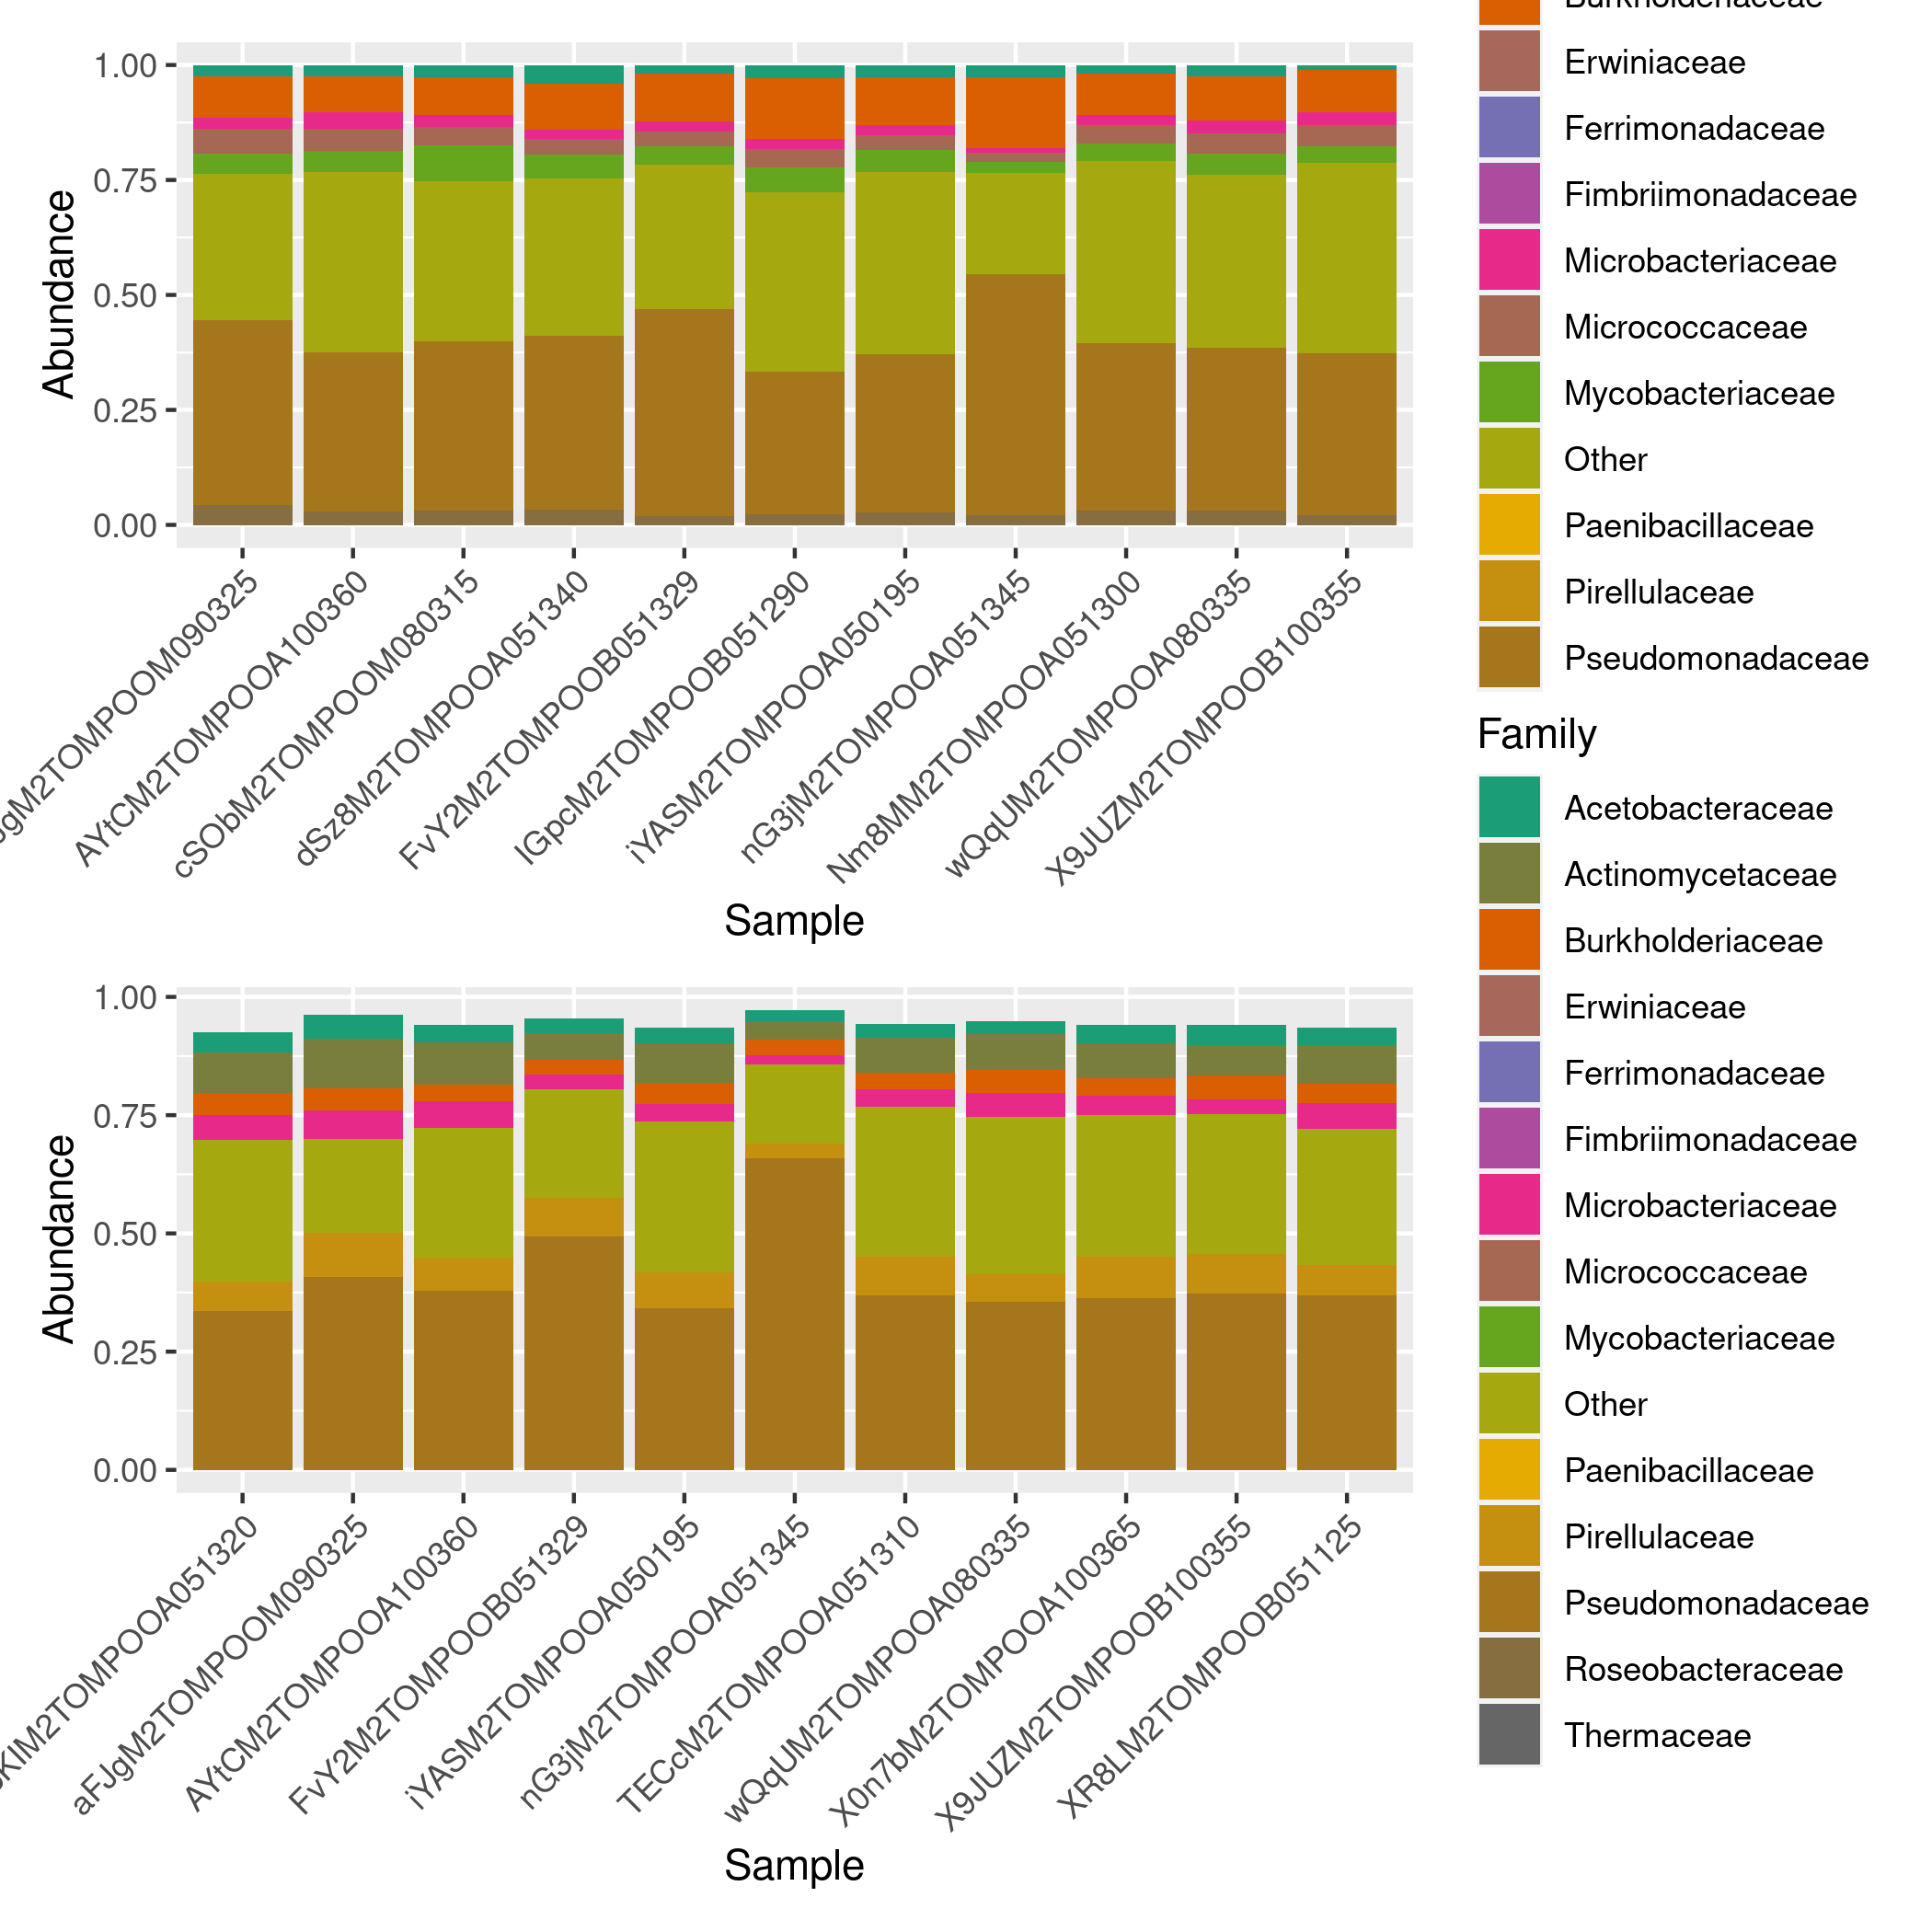
\includegraphics[scale=0.8]{otus_centrales_tomate_aleatorio1_5.csv_otus_centrales_tomate_aleatorio1_6.csv_relative_abundance_Family.png}
\caption{Comparison of reports from random subsamples 5 and 6 by Phylum}
\end{figure}


\begin{figure}
\centering
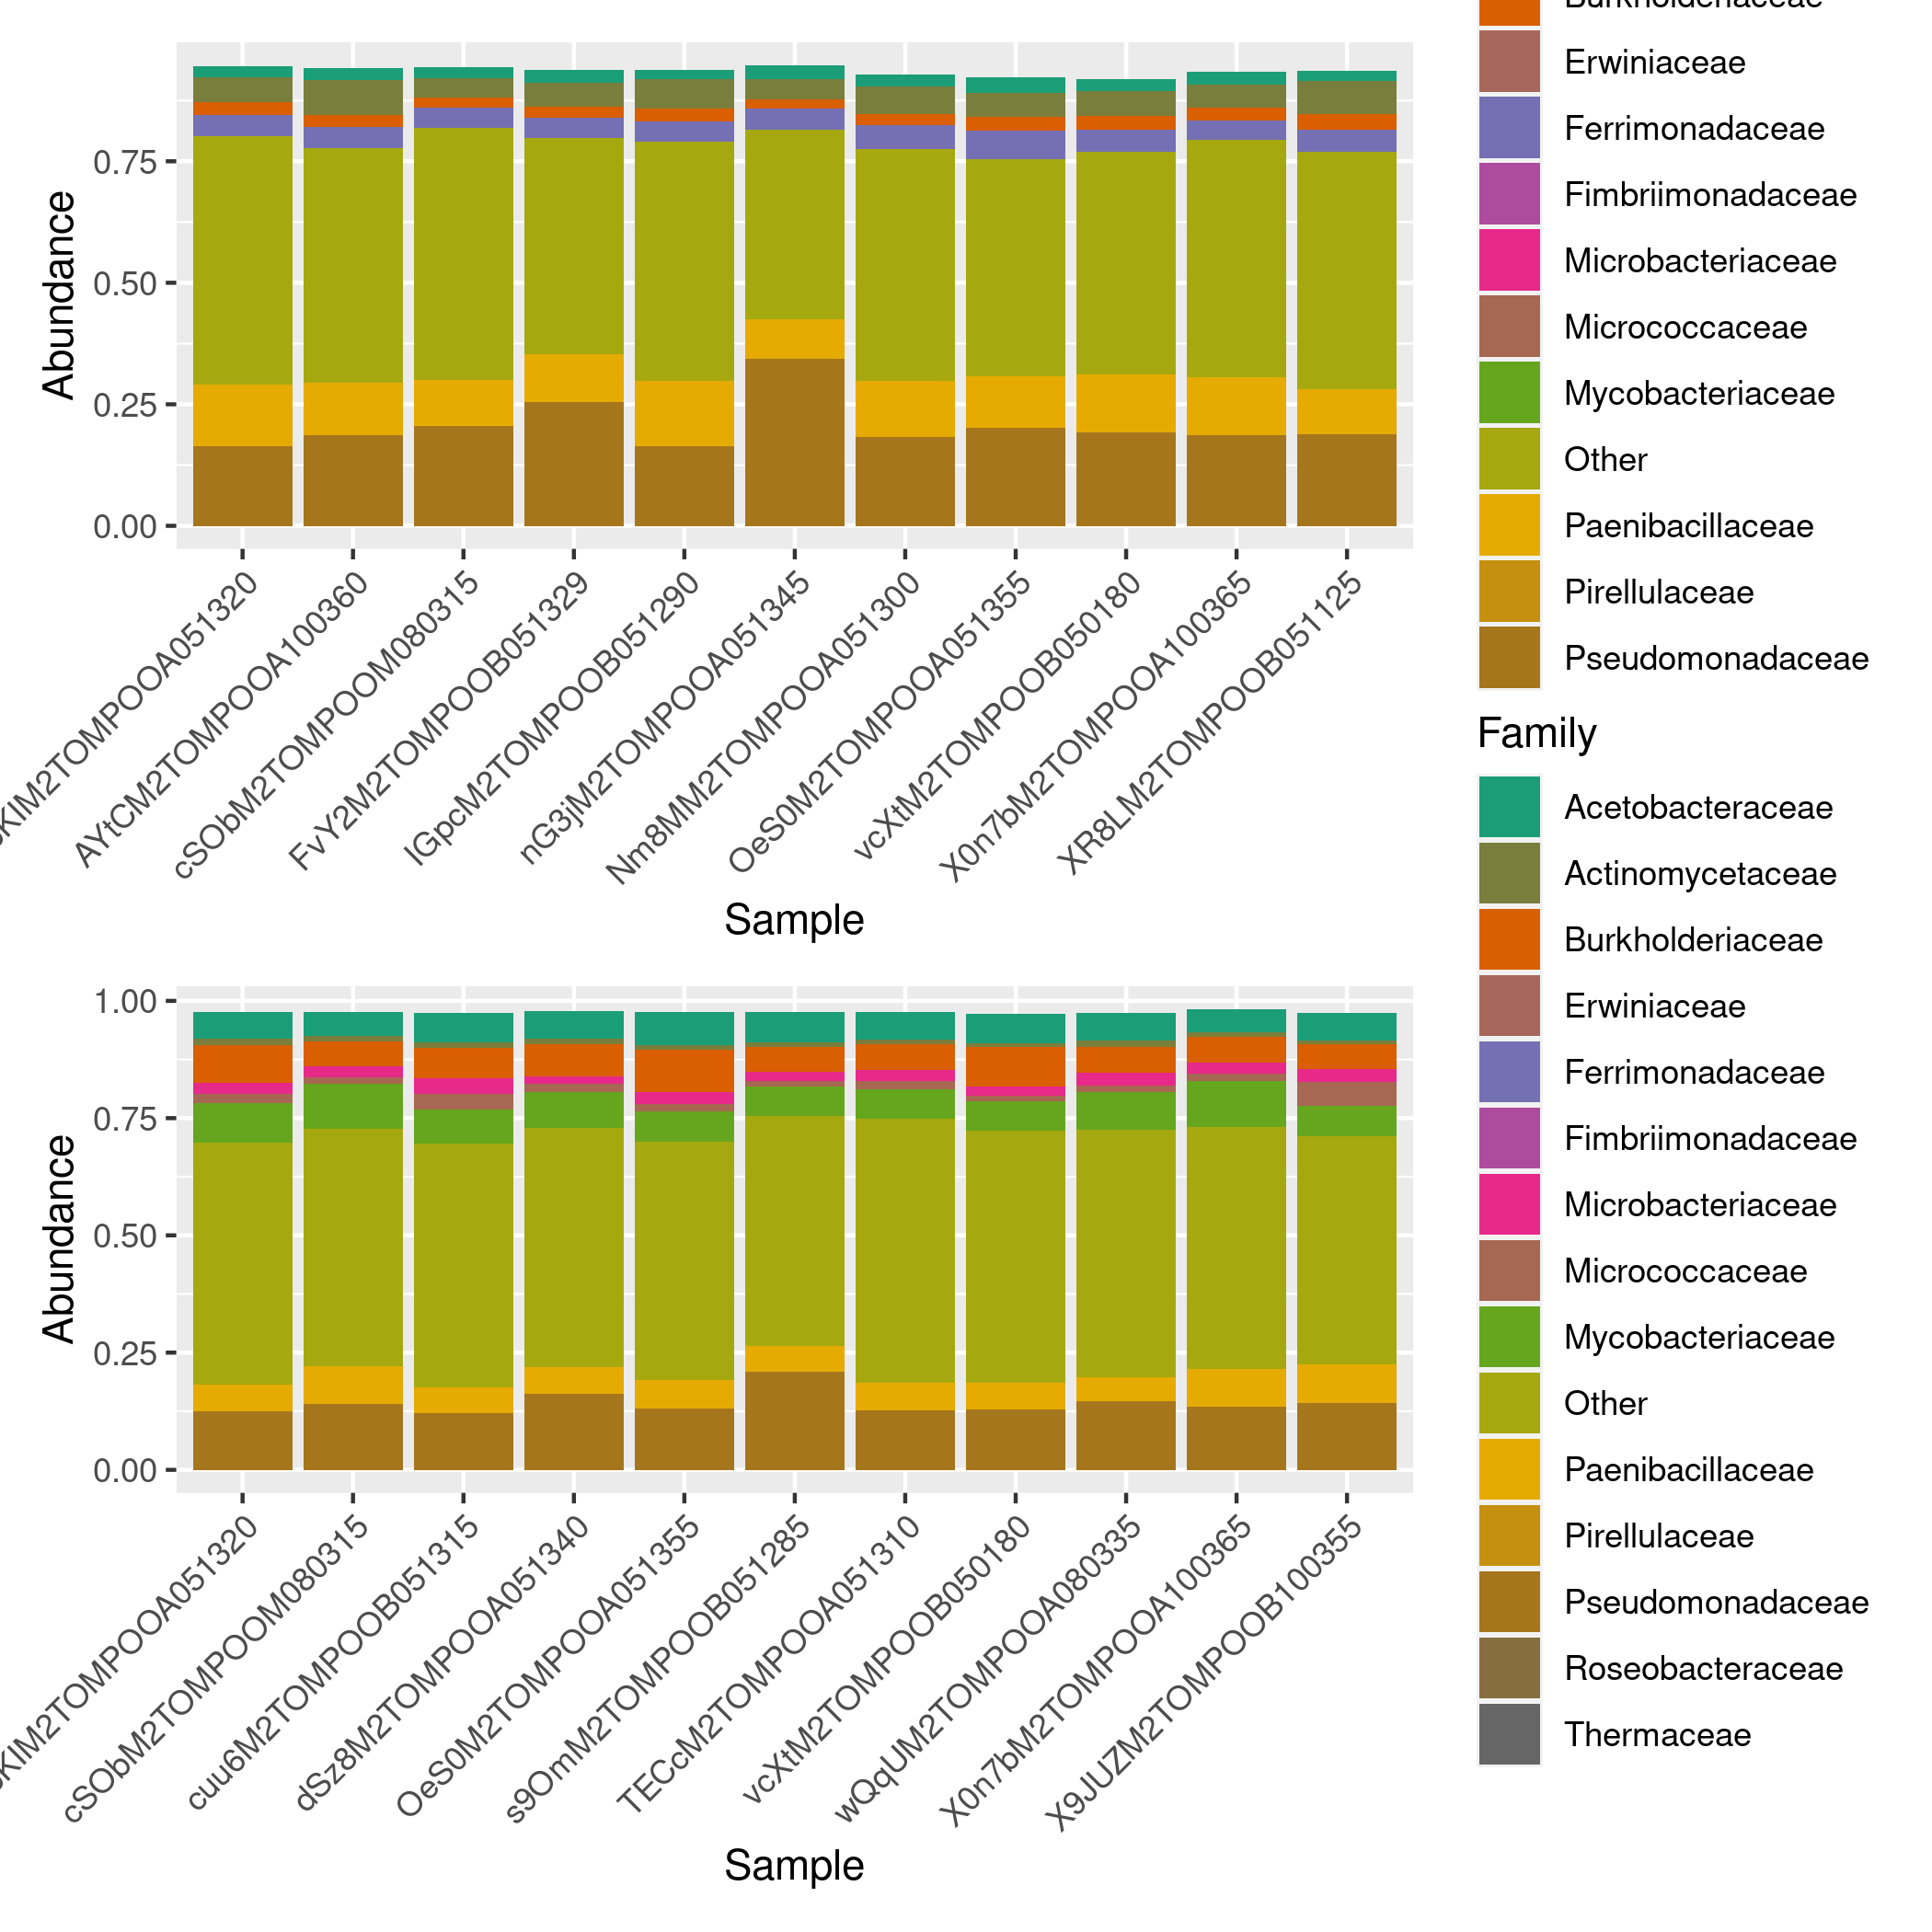
\includegraphics[scale=0.8]{otus_centrales_tomate_aleatorio1_7.csv_otus_centrales_tomate_aleatorio1_8.csv_relative_abundance_Family.png}
\caption{Comparison of reports from random subsamples 7 and 8 by Phylum}
\end{figure}


\begin{figure}
\centering
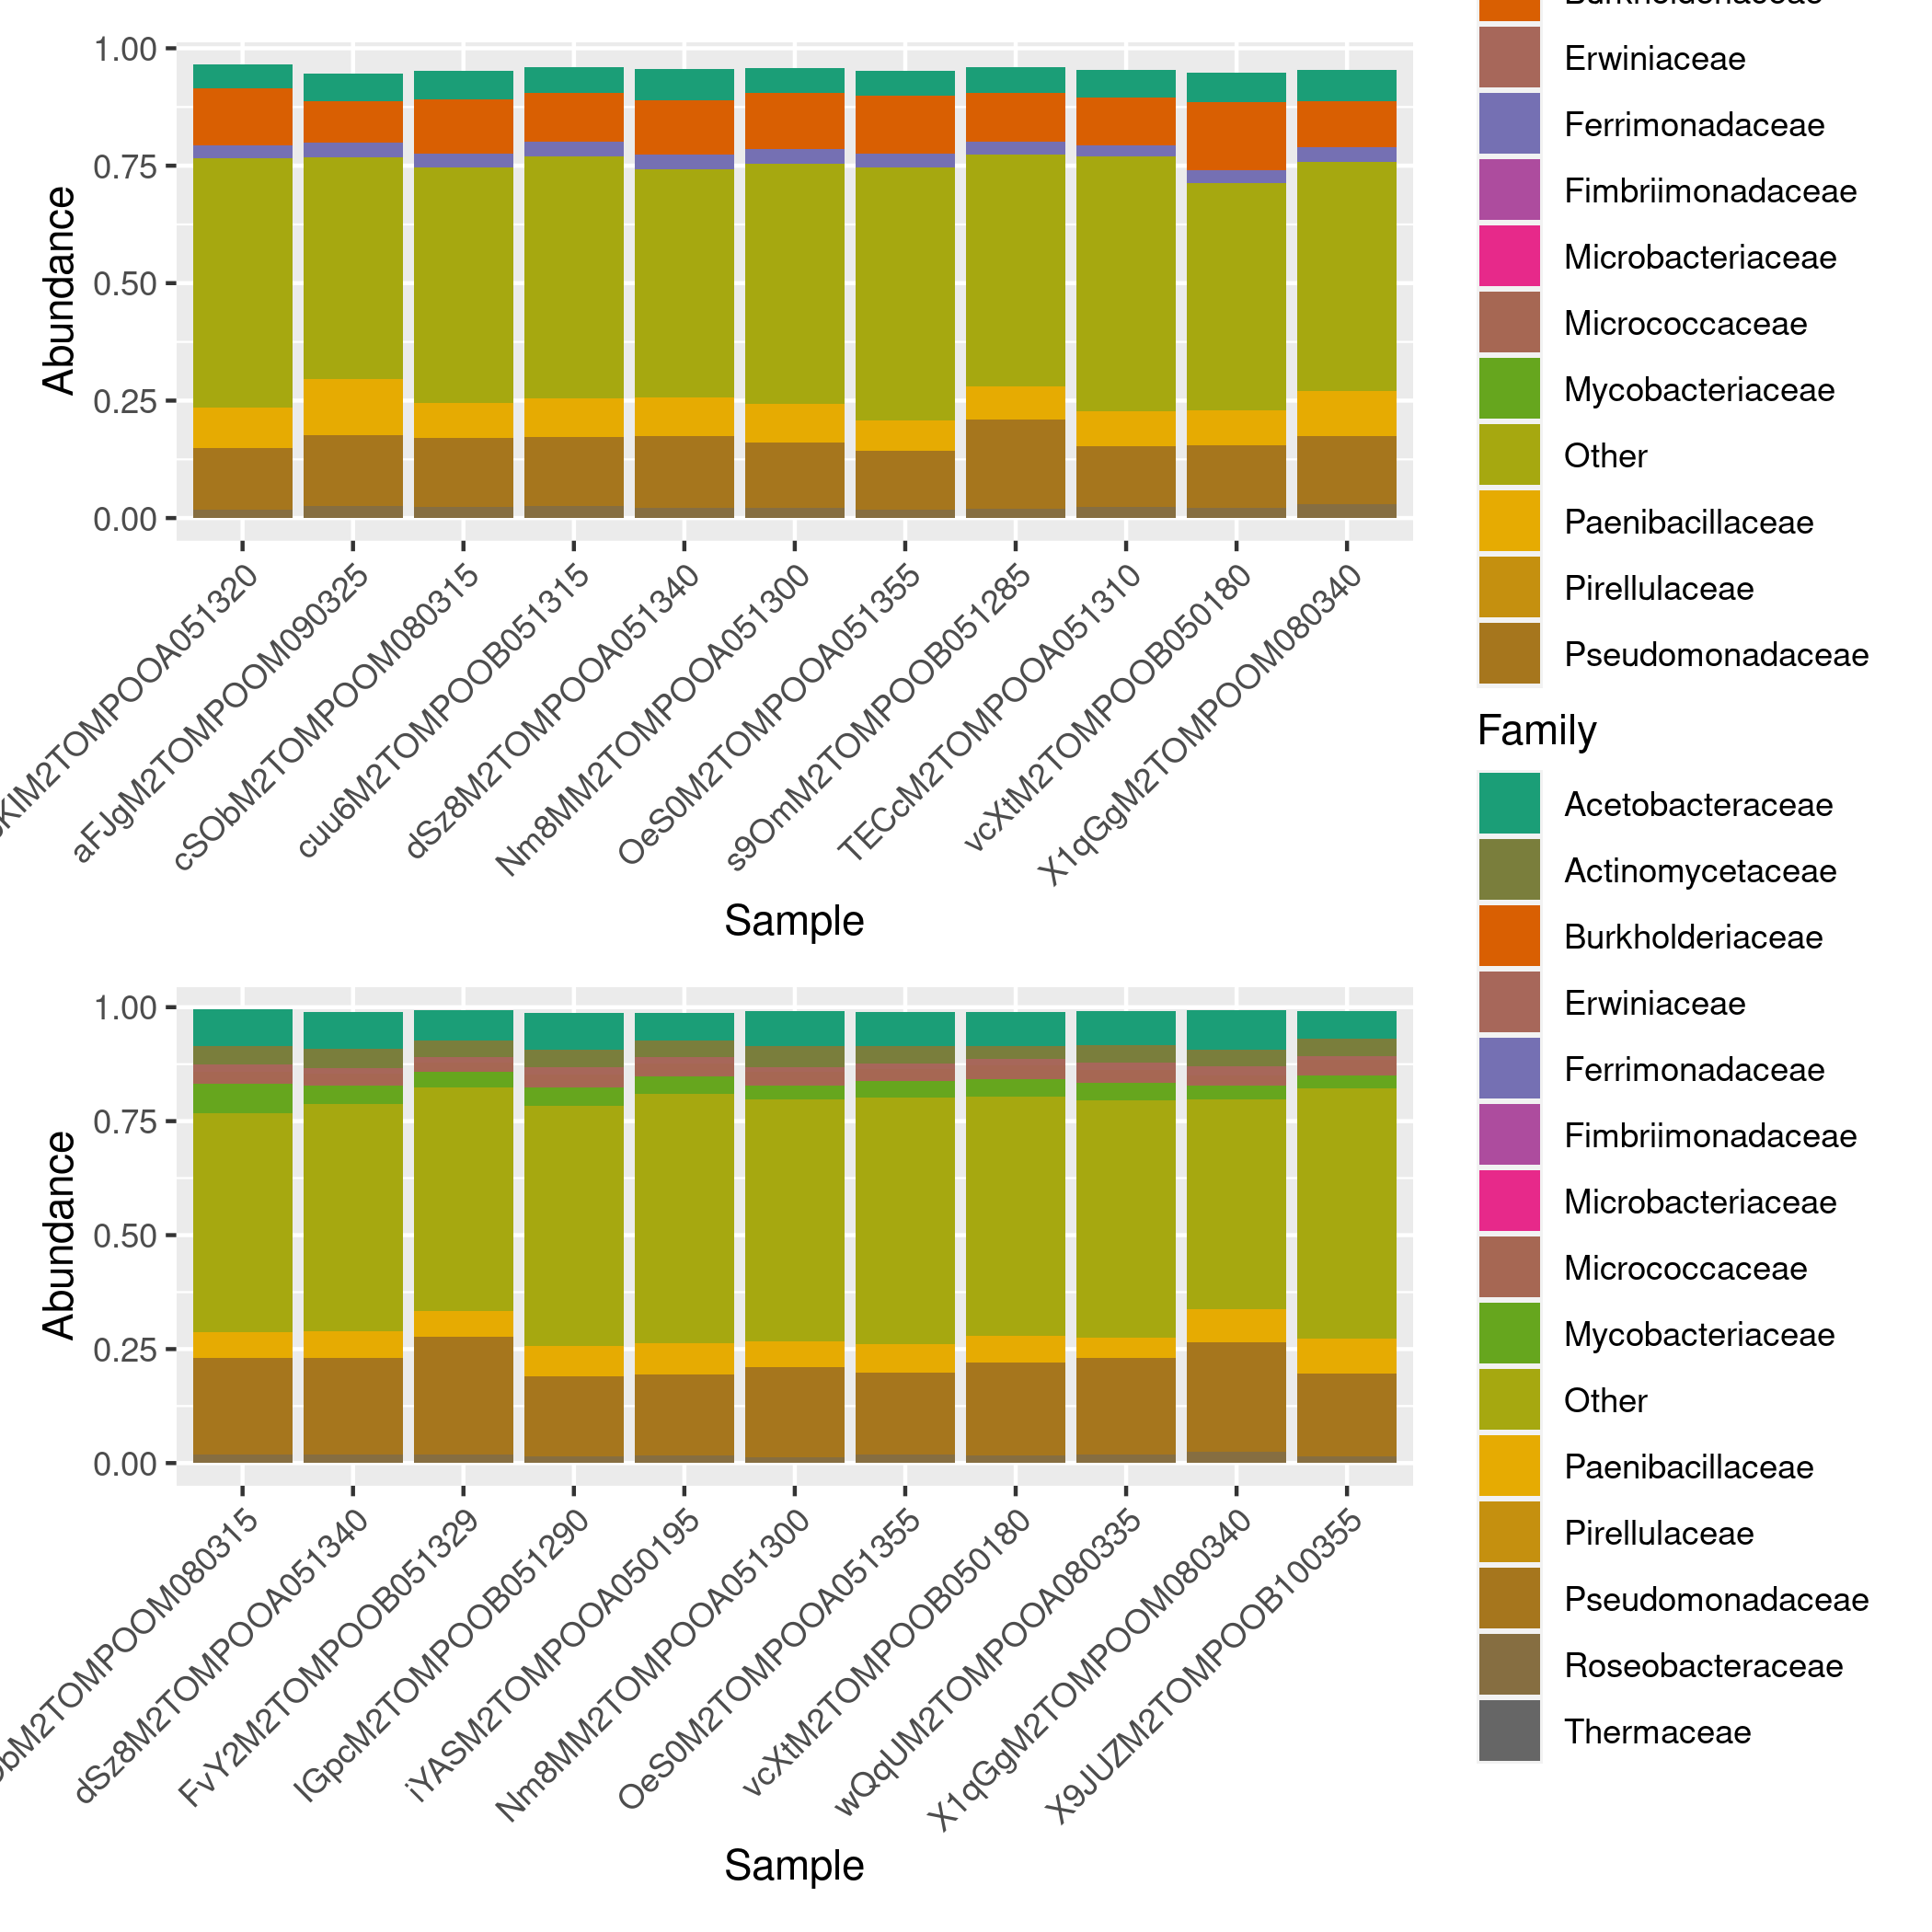
\includegraphics[scale=0.8]{otus_centrales_tomate_aleatorio1_1.csv_otus_centrales_tomate_aleatorio1_2.csv_relative_abundance_Family.png}
\caption{Comparison of reports from random subsamples 9 and 10 by Phylum}
\end{figure}

\begin{figure}
\centering
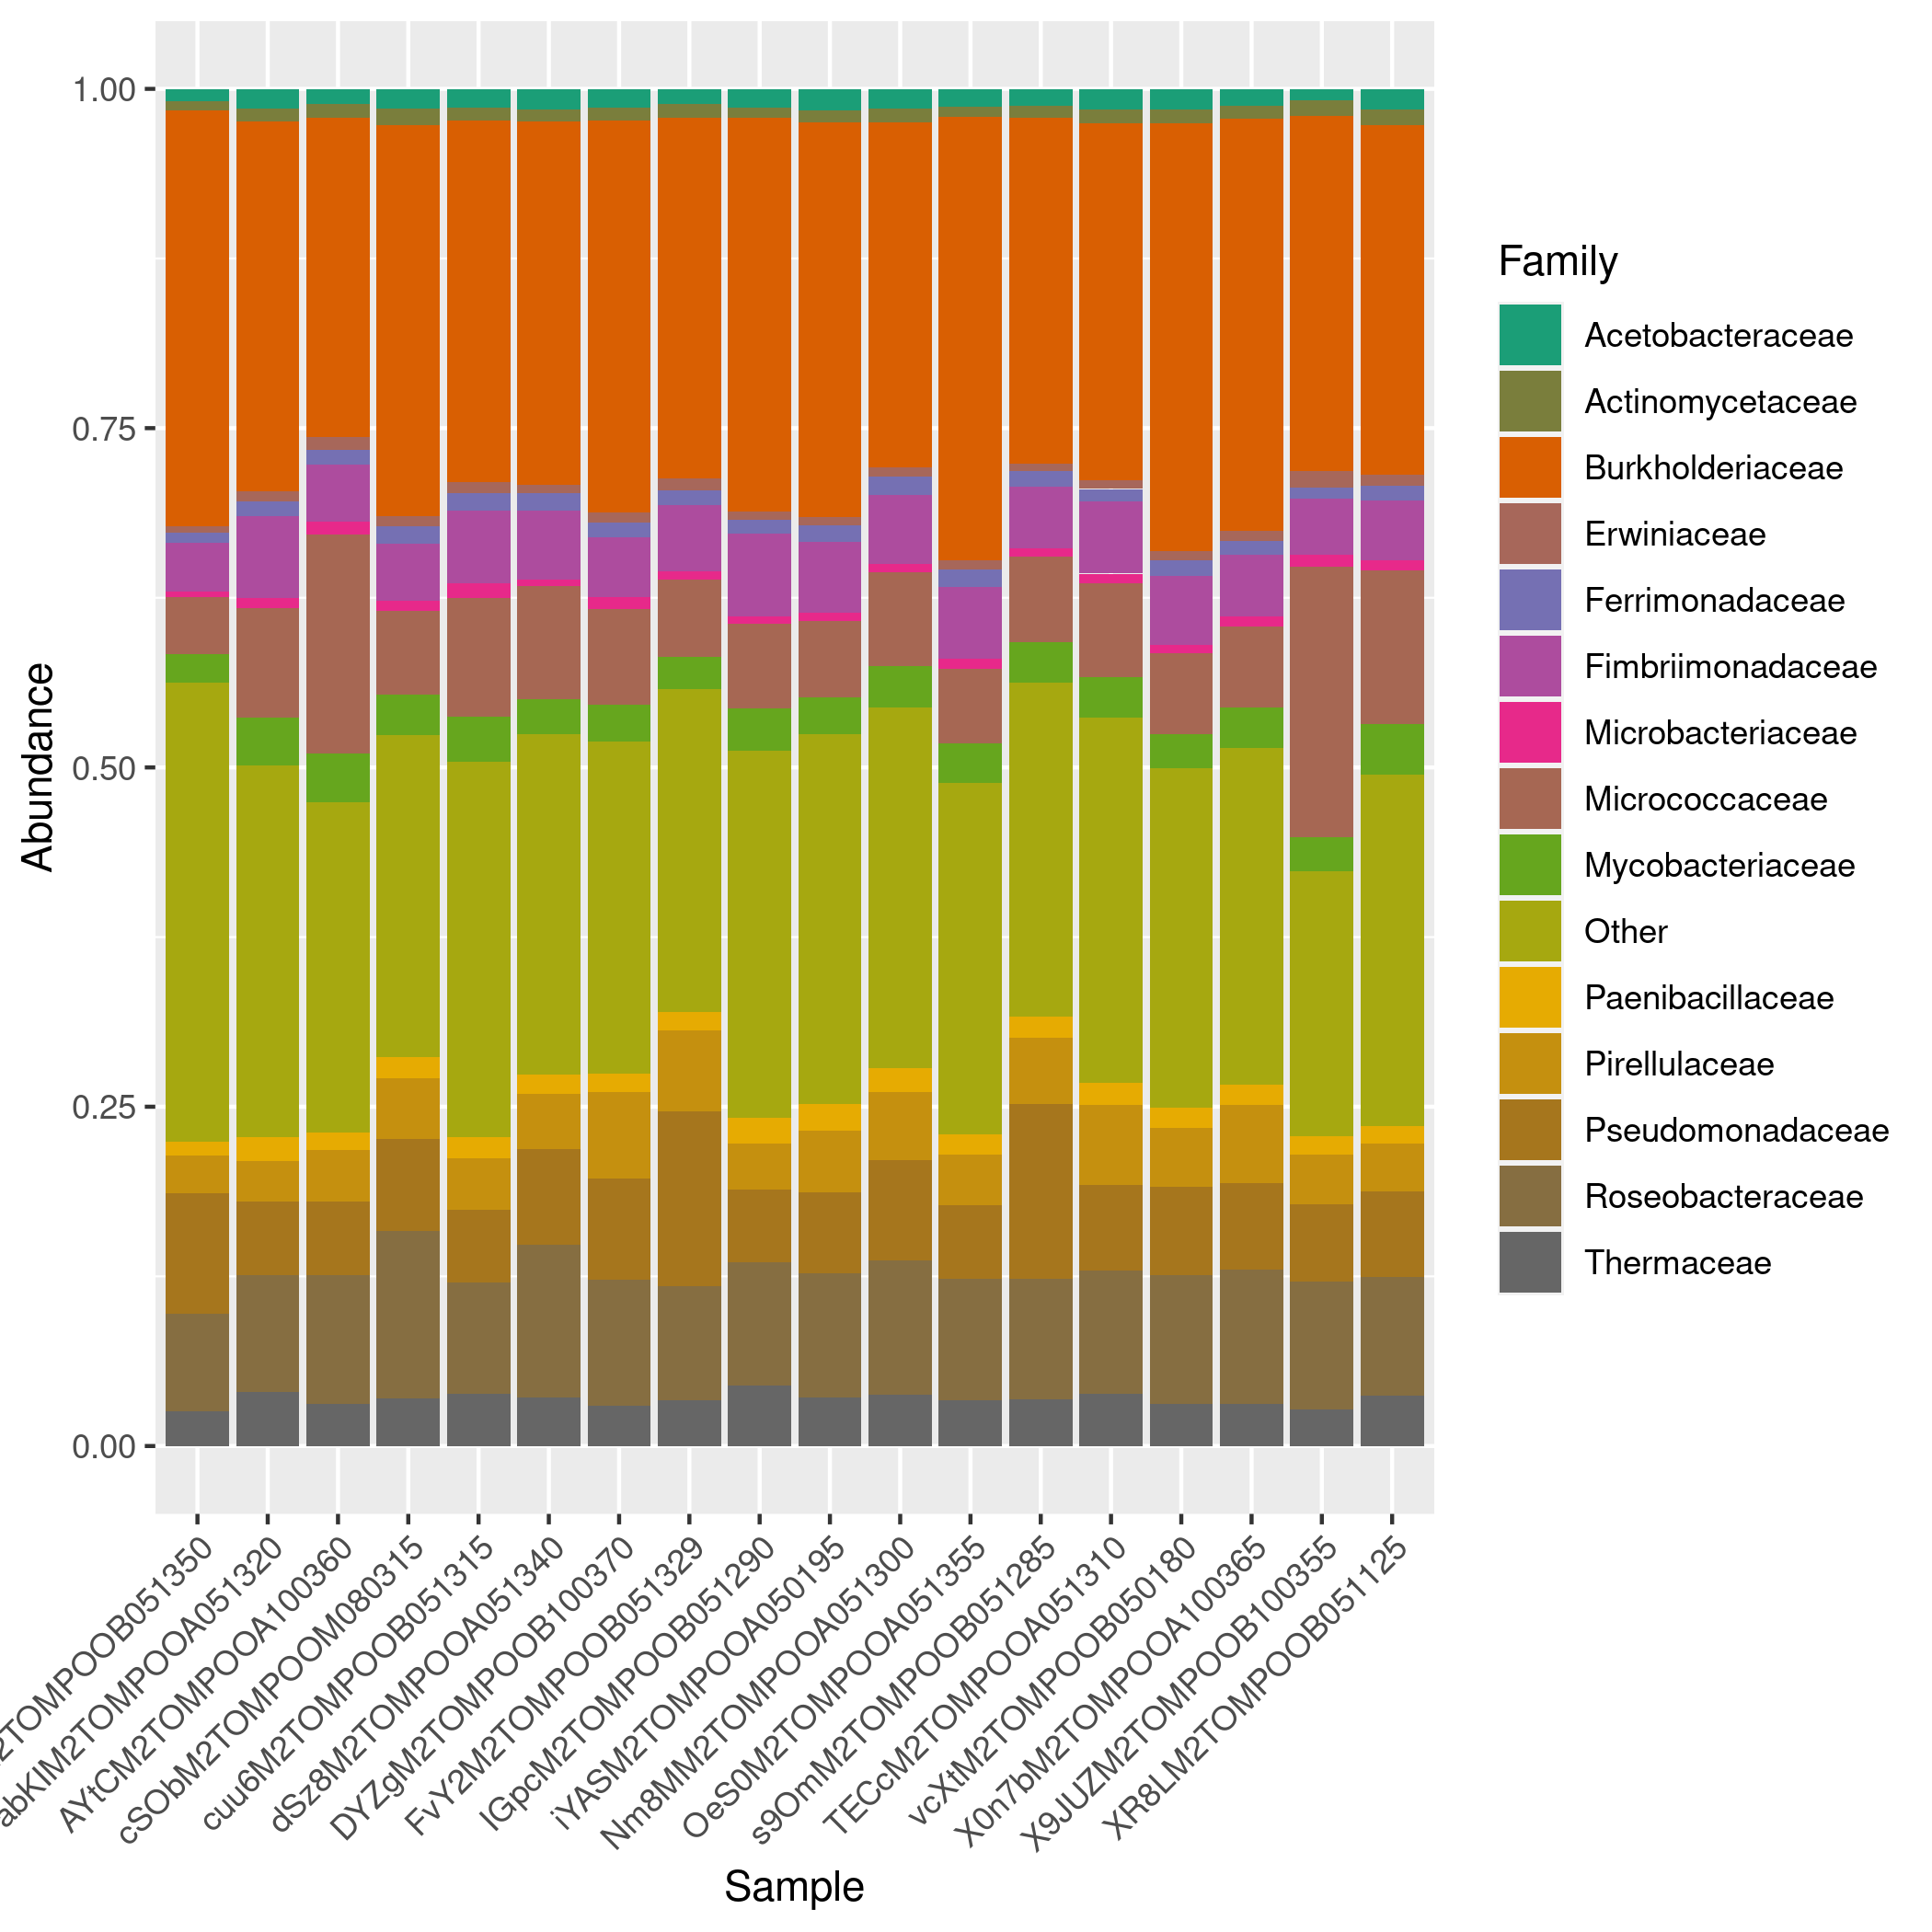
\includegraphics[scale=0.8]{reporte_tomate1.csv_NA_relative_abundance_Family.png}
\caption{Comparison of reports from random subsamples 9 and 10 by Phylum}
\end{figure}


\end{document}